\seccion{Unos ejemplos y aplicaciones}
\label{Sec:SZ:Ejemplos}

% ================================= MaxEnt

\subseccion{El principio de entrop\'ia m\'axima}
\label{Ssec:SZ:MaxEnt}

En  la  termodin\'amica, el  estudio  de  las caracter\'isticas  macrosc\'opicas
(din\'amica de las mol\'eculas) es prohibitivo tan el n\'umero de mol\'eculas es
importante. Por  ejemplo, un litro del  gas que respiramos  contiene $2.7 \times
10^{22}$  mol\'eculas.   De  esta  constataci\'on  se  desaroll\'o  la  f\'isica
estad\'isticas    bajo   el    impulso    de   Boltzmann~\cite{Bol96,    Bol98},
Maxwell~\cite{Max67},  Gibbs~\cite{Gib02}, Planck~\cite{Pla15} entre  otros (ver
tambi\'en~\cite[y   ref.]{Jay65,  Mer10,   Mer18}),   considerando  el   sistema
macrosc\'opico  a  trav\'es de  lo  que  llamaron  ensembles estad\'isticos:  el
sistema  global  (macrosc\'opico)  es  al equilibrio  pero  las  configuraciones
(micro-estados)  son  fluctuantes.   De  una  forma,  se  puede  asociar  a  una
configuraci\'on su  frecuencia de ocurrencia (imaginando tener  une infinidad de
copias del sistema en el  mismo estado macrosc\'opico), es decir su probabilidad
de occurencia (ver  secci\'on~\ref{Ssec:MP:FamiliaExponencial}).  En este marco,
la entrop\'ia, describiendo la falta de informaci\'on, juega un rol fundamental.
Un sistema  sujeto a v\'inculos, como  por ejemplo teniendo  una energ\'ia dada,
debe estar  en sus estado  lo m\'as desorganizado  dados los v\'inculos.   En su
marco, se introdujo la noci\'on  de entrop\'ia termodin\'amica, pero la misma es
tremendamente vinculada a la  entrop\'ia de Shannon~\footnote{Ver ep\'igrafe del
  cap\'itulo\ldots} (claramente, identificando  las frecuencias a probabilidades
de  ocurrencia).    En  otros  terminos,  la   distribuci\'on  describiendo  los
micro-estados  debe  ser de  entrop\'ia  m\'axima,  dados  los v\'inculos.   Por
ejemplo,  en un  gas perfecto,  donde  las part\'iculas  no interactuan  (aparte
chocandose), la  energ\'ia es dada por  las velocidades (suma  de las energ\'ias
cin\'eticas individuales).   Dada una energ\'ia  fija, la distribuci\'on  de las
velocidades debe  ser de  entrop\'ia m\'axima sujeto  a la energ\'ia  dada (nada
m\'as  que  la  energ\'ia  va  a ``organizar''  las  configuraciones  posibles).
Intuitivamente, en  un sistema aislado de $N$  part\'iculas, las configuraciones
van  a   ser  equiprobables,  precisamente  la   distribuci\'on  maximizando  la
entrop\'ia.   \SZ{ En  la  subsecci\'on Sec.~\ref{Ssec:SZ:GasPerfecto}  se va  a
  desarollar un poco m\'as este ejemplo.}

De manera general, el problema se  formaliza como la b\'usqueda de la entrop\'ia
m\'axima  sujeto  a  v\'inculos.    Si  este  principio  naci\'o  en  mec\'anica
estad\'istica  (ver  tambi\'en~\cite{Jay57,   Jay57:2,  Jay65,  Mer10,  Mer18}),
encontr\'o  un  echo en  varios  campos:  en  inferencia bayesiana  para  elegir
distribuciones del a  priori~\footnote{Ver notas de pie~\ref{Foot:MP:BayesPrior}
  y~\ref{Foot:MP:BayesPriorConjugado}.    Recuerdense  que   en   la  inferencia
  bayesiana de un par\'ametro modelizado como aleatorio $\theta$, para eligir la
  ley a  priori \ $p_\Theta(\theta)$, si  se conocen momentos por  una raz\'on o
  una otra,  se puede elegir  esta distribuci\'on como la  ``menos informativa''
  posible,  \ie de  entrop\'ia m\'axima  dados los  momentos.}   conociendo unos
momentos  de  la  ley~\cite{Rob07,  Jay68,  Jay82,  Csi91},  hacer  estimaci\'on
espectral o de procesos estoc\'asticos autoregresivos~\cite{Bur67, Bur75, Jay82}
o~\cite[cap.~12]{CovTho06}, entre otros~\cite[\& ref.]{Arn01, Kap89, KapKes92}.

Sea \ $X$ \ variable aleatoria viviendo sobre (de distribuci\'on de probabilidad
de soporte) \  $X(\Omega) = \X \subset \Rset^d$  \ con \ $K \ge 0$  \ momentos \
$\Esp\left[ M_k(X)  \right] = m_k$ \  fijos, con $M_x: \X  \to \Rset$. Suponemos
que  $X$  tiene  una  densidad  \  $p$  \  con  respecto  a  una  medida  $\mu$,
basicamente  \  $\mu_L$  \  en  el  contexto continuo  y  $\mu_\X$  en  el  caso
discreto. El problema de entrop\'ia m\'axima  se formula de la manera siguiente:
sean \ $M(x) =  \begin{bmatrix} M_1(x) & \cdots & M_K(x)  \end{bmatrix}^t$ \ y \
$m =  \begin{bmatrix} m_1  & \cdots  & m_K \end{bmatrix}^t$  (si $K  = 0$  \ $M$
desaparece)
%, \:
% M = m = 1$), \ se busca,
%
\[
p_{\mathrm{em}}  =   \argmax_p  H(p)  \qquad   \mbox{sujeto  a}  \qquad   p  \ge
0, \quad \int_\X p(x) \, d\mu(x) = 1 \quad \mbox{y}
\quad \int_\X M(x) \, p(x) \, d\mu(x) = m,
\]
%
donde los dos primeros v\'inculos (positividad, normalizaci\'on) aseguran de que
$p_{\mathrm{em}}$ sea una distribuci\'on de  probabilidad. En el ejemplo del gas
perfecto, $K  = 1,  \, M_1(x) =  \frac12 m  \sum_i x_i^2$ \  (los $x_i$  son las
velocidades).   Con  la t\'ecnica  del  Lagrangiano  para  tomar en  cuenta  los
v\'inculos,   introduciendo   factores   de   Lagrange   $\eta_0,   \quad   \eta
= \begin{bmatrix}  \eta_1 &  \cdots &  \eta_K \end{bmatrix}^t$  \ para  tener en
cuenta  los  v\'inculos,  el  problema   variacional  consiste  a  maximizar  la
integral~\cite{GelFom63, Bru04, Mil00, CamMar09, CovTho06}
%
\[
p_{\mathrm{em}} =  \argmax_p \int_\X \left(  - p(x) \log  p(x) + \eta_0  \, p(x)
  + \eta^t M(x) \, p(x) \right) d\mu(x),
\]
%
donde $\eta_0, \eta$  ser\'an determinados para satisfacer a  los v\'inculos. Se
puede ver que el problema es c\'oncava  con respecto a $p$ (\ie el integrande es
una funci\'on  c\'oncava de  $p$), as\'i  que existe  una soluci\'on  \'unica al
problema~\cite{GelFom63, Wei74,  Bru04, Mil00,  CamMar09, Cla13, Kom14}.   En el
caso continuo $\mu = \mu_L$ se usa la ecuaci\'on de Euler-Lagrange~\footnote{En
el caso  discreto, queda claro  que los $p_i$  se buscan anulando  las derivadas
parciales. En  el caso  continuo, el problema  es un  extremizaci\'on functional
conocida como problema variacional.  En el  caso general inicial, el problema es
extremizar $\displaystyle \I[f]  = \int_\X \L\left( x , f(x)  , f'(x) \right) \,
dx$ \ con  \ $\L(x,u,v) \in C^1\left(  \Rset^3 , \Rset \right)$.   Si el calculo
variacional  es debido  a I.   Newton o  G.  W.   Leibniz, los  primeros que  se
enfocaron en tales problemas de optimizaci\'on variacionales fueron los hermanos
J.      Bernoulli~\cite{Ber1697,     Ber1701,    Ber1718}     (ver     tambi\'en
I. Newton~\cite{New1696}),  L.  Euler~\cite{Eul1738,  Eul1744, Eul1766}  y luego
J. L.   Lagrange~\cite{Lag1760:1, Lag1760:2,  Lag1766} a  partir del  trabajo de
Euler~\cite{Gol80, Fra92, Fra94, BraSan07}, por  ejemplo en problemas de buscada
de   camino   m\'inimo   (en   termino   de  tiempo)   entre   dos   puntos   en
mec\'anica.  Volviendo  a  la  extremiezaci\'on,  si $f_e$  es  el  extremo,  se
escribe  \   $f  =  f_e   +  \delta  f$   \  y  se   hace  un  desarollo   de  \
$\L(x,f(x),f'(x))$  \ en  $\delta$ para  obtener  que $f_e$  debe satisfacer  la
famosa       ecuaci\'on       (diferencial)      de       Euler-Lagrange       \
$\displaystyle        \frac{\partial         L}{\partial        u}(x,f(x),f'(x))
- \frac{d}{dx}  \left(  \frac{\partial  L}{\partial v}(x,f(x),f'(x))  \right)  =
0$.    Ver    m\'as   adelante    la    extensi\'on    multivariada   de    esta
ecuaci\'on.\label{Foot:SZ:EulerLagrange}}~\cite{GelFom63,  Wei74, Bru04,  Cla13,
Kom14}, esquematicamente anulando la ``derivada''  del integrande con respecto a
$p$; en  el caso discreto,  se anula realmente un  gradiente con respecto  a los
componentes de $p$. Eso da que $p$ debe satisfacer a la ecuaci\'on
%
\[
- \log p(x) - 1 + \eta_0 + \eta^t M(x) = 0
\]
%
Reparametrizando los factores de Lagrange, se obtiene as\'i
%
\[
p_{\mathrm{em}}(x) = \frac{1}{Z(\eta)} e^{\eta^t M(x)} = e^{\eta^t M(x) - \varphi(\eta)},
\]
%
con $\eta$  tal que  se satisfacen  los v\'inculos  de momentos  y \  $Z(\eta) =
e^{\varphi(\eta)} =  \displaystyle \int_\X e^{\eta^t M(x)}  d\mu(x)$ coeficiente
de  normalizaci\'on.   Esta  distribuci\'on   cae  precisamente  en  la  familia
exponencial  que hemos  visto secci\'on~\ref{Ssec:MP:FamiliaExponencial},  donde
$M$ es  la estad\'istica suficiente y  $\eta$ el par\'ametros naturale  (en este
caso, $h(x) = 1$). Adem\'as, la entrop\'ia m\'axima se obtiene inmediatamente de
$\log p_{\mathrm{em}} = \eta^t M - \varphi(\eta)$.
%
%\[
%\max_p H(p) = H(p_{\mathrm{em}}) = - \eta^t m + \varphi(\eta)
%\]

Un problema que puede  aparecer es que no se puede determinar  $\eta$ tal que se
satisfacen todos los  v\'inculos, en particular se puede que  no se normaliza la
ley.  Por ejemplo,  si $\X = \Rset$ y  $K = 0$, \ $p$ \  deber\'ia ser constante
(ley  uniforme) sobre\ldots  $\Rset$, lo  que no  es normalizable.  De  la misma
manera, si $K  = 3$ \ y \  $M_k(x) = x^k$, tampoco es  normalizable la funci\'on
obtenida~\footnote{En el  enfoque bayesiano se puede que  no sea problem\'atico,
  si el  a posteriori es normalizable~\cite{Rob07},  pero va m\'as  all\'a de la
  meta de  esta secci\'on.}.  En  otros terminos, en  este caso, el  problema no
tiene soluci\'on~\footnote{M\'as  precisamente, existen  casos en los  cuales se
  puede acotar la entrop\'ia por arriba  por un $H^{\sup}$, tal que $\sup_p H(p)
  \le H^{\sup}$ pero no  se puede alcanzar esta cota, \ie es  un supremum, no un
  m\'aximo~\cite[sec.~12.3]{CovTho06}.}.

Existe   una  prueba   informacional   de  este   resultado,   saliendo  de   la
soluci\'on.
%
\begin{lema}
\label{Lem:SZ:MaxEntPruebaInfo}
%
  Sea \  $\displaystyle \P_m =  \left\{ p  \ge 0 \tq  \int_\X p(x) \,  d\mu(x) =
  1,  \quad  \int_\X M(x)  \,  p(x)  \, d\mu(x)  =  m  \right\}$ \  conjunto  de
  densidades  con respecto  a $\mu$,  con los  mismos momentos  \ $M$,  y sea  \
  $p_{\mathrm{em}}  \in \P_m$  \ que  sea de  la forma  \ $p_{\mathrm{em}}(x)  =
  e^{\eta^t M(x) - \varphi(\eta)}$. Entonces
  %
  \[
  \forall  \,  p \in  \P_m,  \quad  H(p) \le  H(p_{\mathrm{em}})  =  - \eta^t  m
  +    \varphi(\eta)    \qquad   \mbox{con    igualdad    ssi}    \quad   p    =
  p_{\mathrm{em}} \quad \mu\mbox{-(c. s.)}, \]
  %
  donde   $H$  es   de  la   definici\'on   general  Def.~\ref{Def:SZ:ShanonMu}
  %pagina~\pageref{Def:SZ:ShanonMu}, 
  de la entrop\'ia con respecto a $\mu$.
\end{lema}
%
\begin{proof}
  \begin{eqnarray*}
  \Dkl[p]{p_{\mathrm{em}}} & = & \int_\X
  p(x) \, \log\left( \frac{p(x)}{p_{\mathrm{em}}(x)} \right) \, d\mu(x)\\[2.5mm]
  %
  & = & - H(p) - \int_\X p(x) \, \log p_{\mathrm{em}}(x) \,  d\mu(x)\\[2.5mm]
  %
  & = & - H(p) - \int_\X p(x) \, \big(  \eta^t M(x) - \varphi(\eta) \big) \,  d\mu(x)\\[2.5mm]
  %
  & = & - H(p) - \int_\X p_{\mathrm{em}}(x) \, \big(  \eta^t M(x) - \varphi(\eta) \big) \,  d\mu(x)\\[2.5mm]
  %
  & = & - H(p) - \int_\X p_{\mathrm{em}}(x) \, \log p_{\mathrm{em}}(x) \,  d\mu(x)\\[2.5mm]
  %
  & = & H(p_{\mathrm{em}}) - H(p)
  %H(p) & = & - \int_\X p(x) \, \log p(x) \, d\mu(x)\\[2.5mm]
  %
  %& = & - \int_\X p(x) \, \log\left( \frac{p(x)}{p_{\mathrm{em}}(x)} \right) \,
  %d\mu(x) - \int_\X p(x) \, \log p_{\mathrm{em}}(x) \, d\mu(x)
  \end{eqnarray*}
  %
  donde en la tercera y la quinta  linea se usa $\log p_{\mathrm{em}} = \eta^t M
  - \varphi(\eta)$,   mientras    que   en   la    quarta   se   usa    qu   $p,
  p_{\mathrm{em}} \in \P_m$ (tienen los mismos momentos).
  %De la positividad de la divergencia de Kullback-Leibler
  %se obtiene
  %
  %\begin{eqnarray*}
  %H(p) & = & - \Dkl[p]{p_{\mathrm{em}}} - \int_\X \left( \eta^t M(x)
  %- \varphi(\eta) \right) p(x) \, d\mu(x)\\[2.5mm]
  %%
  %& = & - \Dkl[p]{p_{\mathrm{em}}} - \int_\X \left( \eta^t M(x)
  %- \varphi(\eta) \right) p_{\mathrm{em}}(x) \, d\mu(x)\\[2.5mm]
  %%
  %& = & - \Dkl[p]{p_{\mathrm{em}}} - \int_\X p_{\mathrm{em}}(x) \log
  %p_{\mathrm{em}}(x) \, d\mu(x)\\[2.5mm]
  %%
  %& = & - \Dkl[p]{p_{\mathrm{em}}} + H(p_{\mathrm{em}})
  %\end{eqnarray*}
  %  
  %porque  $p,  p_{\mathrm{em}}  \in  \P_m$  \ (segunda  linea)  y  \  $\eta^t  M
  %- \varphi(\eta) = \log  p_{\mathrm{em}}$ (tercera linea).
  La  prueba se cierra
  notando que $\Dkl[p]{p_{\mathrm{em}}} \ge 0$ con igualdad si y solamente si $p
  =  p_{\mathrm{em}}  \quad  (\mu$-c.s.).\newline  La  forma  de  la  entrop\'ia
  m\'axima  sale  inmediatamente de  $  -  p_{\mathrm{em}} \log  p_{\mathrm{em}}
  = \left( - \eta^t M + \varphi(\eta) \right) \, p_{\mathrm{em}}$.
\end{proof}
%
Este lema prueba que, dados  v\'inculos ``razonables'', la entrop\'ia es acotada
por  arriba, y que  se alcanza  la cota  para una  distribuci\'on de  la familia
exponencial. Por ejemplo,
%
\begin{itemize}
\item Con  $K =  0$ \  y \  $\X$ \ de  volumen finito  \ $|\X|  < +  \infty$, la
  distribuci\'on  de entrop\'ia  m\'axima es  la distribuci\'on  uniforme de  la
  propiedad~\ref{Prop:SZ:cotamaximauniforme}     \     de    la     subsecci\'on
  Sec.~\ref{Ssec:SZ:Diferencial}      en      el      caso      continuo,      o
  propiedad~\ref{Prop:SZ:cotamaxima}        \       de        la       secci\'on
  Sec.~\ref{Ssec:SZ:DefinicionShannon} en el caso discreto.
%
\item Con $K = 1$,  \ $\X = \Rset^d$ \ y \ $M(x) = x  x^t$ (visto como $K = d^2$
  momentos),  la  distribuci\'on de  entrop\'ia  m\'axima  es la  distribuci\'on
  gausiana de  la propiedad~\ref{Prop:SZ:cotamaximagaussiana} \  de la secci\'on
  Sec.~\ref{Ssec:SZ:Diferencial}.
\end{itemize}
%
Con el enfoque del lema~\ref{Lem:SZ:MaxEntPruebaInfo}, se necesita solamente que
$p$  sea una  densidad con  respecto  a una  medida $\mu$  fija, cualquiera.   En
particular, si es una medida de probabilidad (de referencia) $\widetilde{P}$, el
problema de entrop\'ia m\'axima vuelve a ser un problema de minimizaci\'on de la
divergencia de Kullback-Leibler entre $P$  y la medida de referencia, siendo $p$
la    densidad    con    respecto     a    esta    medida    (ver    definici\'on
Def.~\ref{Def:SZ:entropiarelativa}). Es decir, tomando \ $\mu = \widetilde{P}$ \
medida de probabilidad aparece inmediatamente\modif{
%
\[
P_{\mathrm{em}} = \argmin_P \Dkl[P]{\widetilde{P}} \quad \mbox{sujeto a} \quad \int_\X
M(x)                       \,                      dP(x) \equiv \int_\X
M(x)    \frac{dP}{d\widetilde{P}}(x)                   \,                      d\widetilde{P}(x)                       =
m
%\qquad
%\Leftrightarrow \qquad  \frac{dP_{\mathrm{em}}}{d\widetilde{P}}(x)  =
%e^{\eta^t M(x) - \varphi(\eta)}.
\]
%
es \'unica, de la forma
%
\[
\frac{dP_{\mathrm{em}}}{d\widetilde{P}}(x)  =
e^{\eta^t M(x) - \varphi(\eta)}.
\]
}

\SZ{Ver como conectar con la minimizaci\'on de entrop\'ia cruzada.}

\modif{

%Se  notar\'a  que   si  $P$  y  $\widetilde{P}$  tienen  una   densidad  $p$  y
%$\widetilde{p}$     con     respecto     a    una     medida     $\mu$,     del
%lema~\ref{Lem:SZ:DescomposicionEntropiaCruzada}, siendo $H(\widetile{p})$ dado,
%minimizar la divergencia \  $\Dkl[p]{\widetilde{p}}$ es equivalente a minimizar
%la entrop\'ia cruzada \ $\Hcruz[\widetilde{p}]{p}$.

\


\index{Estadistica   de    Boltzmann}   \index{Estadistica   de   Bose-Einstein}
\index{Estadistica de Fermi-Dirac}  Vamos a ilustrar este principio  ahora en el
tema  f\'isico   de  ocupaci\'on   de  niveles  de   energ\'ia  en   un  sistema
cerrado~\cite{LanLif80, Mer18}
%
\begin{ejemplo}[Estadistica de ocupaci\'on de niveles energeticos]
  Consideramos un sistema  con niveles de energ\'ia \ $\E_i$  (n\'umero finito o
  infinito de niveles). Supenomos que  haya $g_i$ estados posibles distinguibles
  con   el  mismo   nivel   de   energ\'ia  $\E_i$;   $g_i$   es  llamado   {\em
  degenerenc\'ia}~\ref{toto}.  Suponemos  que el  sistema tiene  $n$ particulas.
  Queremos estudiar  la probabilidad (o  el n\'umero promedio de  particulas) de
  ocupaci\'on  de  cada nivel  de  energ\'ia.   Vamos  ahora a  considerar  tres
  situaciones para describir tal distribuci\'on de probabilidad.

  {\bf Enfoque de Boltzmann:} suponemos  que las particulas son distingables. Es
  decir que, por  ejemplo tener solamente la particula n\'umero  $k$ en en nivel
  $i$  o solamente  la n\'umero  $l\ne k$  en este  nivel son  dos micro-estados
  distinctos.   Eso  es   ilustrado   figura~\ref{Fig:SZ:BBEFD}-(a),  donde   se
  representan todos los microestados posibles para $n_i = 2, g_i = 3$.  Llamamos
  $p_{i,j}$ la probabilidad para una particula  de estar en estado $j$ del nivel
  de  energ\'ia $i$.   Seg\'un  el  principio de  entrop\'ia  maxima, sujeto  al
  v\'inculo de  normalisaci\'on, y  el de  energ\'ia total/promedia  del sistema
  $\Esp[\E(x)] =  \sum_{i,j} p_{i,j}  \E_i$, con la  tecnica del  Lagrangiano que
  v\'imos anteriormente, queremos resolver el problema de maximizaci\'on
  %
  \[  
  p_{\mathrm{em},i,j}  =  \argmax_{p_{i,j}}  \left( -  \sum_{i,j}  p_{i,j}  \log
    p_{i,j}    -    \alpha    \sum_{i,j}     p_{i,j}    -    \beta    \sum_{i,j}
    p_{i,j} \E_i \right) \]
  %  
  Anulando la derivada en cada $p_{i,j}$ conduce a la probabilidad de la familia
  exponencial, \ $p_{\mathrm{em},i,j} = \frac{1}{Z(\beta)} e^{-\beta \, \E_i}$ \
  con, \ $\beta$  \ dado, \ $Z$ \  es la constante de normalizaci\'on  y luego \
  $\beta$ \ es tal que se obtiene  el v\'inculo de energ\'ia, como lo v\'imos en
  esta  secci\'on y  en la  secci\'on~\ref{Ssec:MP:FamiliaExponencial}.  Si  nos
  focalizamos  en  la   distribuci\'on  $p_i$  de  los   niveles  de  energ\'ia,
  escribiendo \ $\mu =  \frac{1}{\beta} \log Z = - F$  (menos la energ\'ia libre
  de  Helmoltz,  o a  veces  conocido  como potencial  qu\'imico~\cite{LanLif80,
  Mer18}) \ se obtiene
  %
  \[  
  p_{\mathrm{em},i}  =  \frac{g_i}{Z(\beta)} \,  e^{-\beta  \,  \E_i} =  g_i  \,
    e^{-\beta \, (\E_i - \mu)} \]
  %
  No  entraremos en  los  detailles,  pero a  partir  de la  primera  ley de  la
  termodin\'amica,  se v\'incula la  energi\'a, la  entrop\'ia y  la temperatura
  $T$, dando
  %
  \[
  \beta  =  \frac{1}{k_B  T}, \qquad  k_B  =  \approx  1.38 \times  10^{-23}  \:
  \mbox{julio por Kelvin, constante de Boltzmann}
  \]
  %
  (ver~\cite{Jay57},~\cite[Cap.~IV]{LanLif80}).

  Se  puedo  obtener esta  distribuci\'on  como  lo hizo  Boltzmann~\cite{Bol96,
    Bol98}, con un enfoque micro-canonico.  Se puede ver los niveles como cajas,
    as\'i  que buscamos  como se  puede repartir  las particulas  en cada  caja.
    Siendo  distinguibles las  particulas, si  tenemos \  $n_i$ \  particulas al
    nivel  \  $\E_i$, existen  \  $g_i^{n_i}$  \ configuraciones  posibles  (ver
    figura~\ref{Fig:SZ:BBEFD}-(a)).  Luego,  con $n$ particulas en  total, si la
    ponemos en una recta para repartirlas en los niveles, diciendo que las $n_1$
    primeras van al  nivel $\E_1$, las $n_2$ siguientes  al nivel $\E_2$,\ldots,
    hay que  considerar las $n!$ permutaciones  posibles en la recta  y tomar en
    cuenta que hay \ $n_i!$ \ de  las permutaciones con las mismas particulas al
    nivel $\E_i$. Es decir que el n\'umero de configuraciones total es
  %
  \[
  W = n! \prod_i \frac{g_i^{n_i}}{n_i!}
  \]
  %
  La entrop\'ia de Boltzmann \ $S = k_B  T \log W$ \ debe ser m\'axima subjeto a
  los v\'inculos del sistema, es decir \  $\sum_i n_i = n, \quad \sum_i n_i \E_i
  = \E$  \ fijo. Se  puede ver en  este problema los  micro-configuraciones como
  uniformamente  distribuidas,  as\'i  que  $1/W$  es la  probabilidad  de  cada
  configuraci\'on  y \  $\log W$  \ representa  la entrop\'ia  a la  Shannon. El
  problema consiste ahora a resolver el problema de maximizaci\'on
  %
  \[  
  n_{\mathrm{em},i}    =   \argmax_{n_i}    \sum_i   \left(    n_i   \log    g_i
    - \log \Gamma(n_i+1) - \alpha n_i - \beta n_i \E_i \right) \]
  %  
  donde \  $p_{\mathrm{em},i} = \frac{n_{\mathrm{em},i}}{n}$ \  va a representar
  la probabilidad  de ocupaci\'on del  nivel $\E_i$.  $n_{\mathrm{em},i}$  no es
  necesariamente    entero,   representando    el   n\'umero    de   ocupaci\'on
  promedio. Ahora, anulando la derivada en cada \ $n_i$ \ conduce a resolver
  %
  \[
  \psi(n_i+1) = \log g_i - \alpha - \beta \, \E_i
  \]
  %  
  con      $\psi$      derivada       de      $\log      \Gamma$,      funci\'on
  digamma~\cite[\S~8.36]{GraRyz15},~\cite[\S~6.3]{AbrSte70}.    Se  supono   que
  $n_i$ es muy grande y se usa el desarollo asimtotico $\psi(n_i+1) = \log n_i +
  o(1)$~\cite[6.3.18]{AbrSte70} para obtener $n_{\mathrm{em},i} = g_i e^{-\alpha
  - \beta \, \E_i}$, que podemos reescribir bajo la forma
  %
  \[
  n_{\mathrm{em},i} = \frac{n \, g_i}{Z(\beta)} \, e^{- \beta \, \E_i}
  \]
  %
  \SZ{Ver aproximaci\'on continua de  Thomas-Fermi, con la degenerancia continua
    \   $g$   \  proportional   a   la  raiz   cuadrada   de   la  energ\'ia   \
    $\sqrt{\varepsilon}$~\cite{Fer28,  Tho27,   LieSim77}  \  conduciendo   a  \
    $p_\E(\varepsilon) \propto \sqrt{\varepsilon} \, e^{- \beta \varepsilon}$ \,
    ley     de     Maxwell-Boltzmann    (ver     secci\'on~\ref{Sssec:MP:Gamma},
    ejemplo~\ref{Ej:MP:MaxwellBoltzmann}).}


  {\bf Enfoque de  Bose-Einstein:} este modelo fue propuesto  por Satyendra Nath
  Bose  en 1924  para explicar~\footnote{En  realidad, la  meta de  Bose  fue de
    probar a sus estudiantes la  inadecuaci\'on del modelo de Boltzmann, pero se
    equivoco en la  aplicaci\'on de esta teoria. Su  ``error'' fue de considerar
    las   particulas   como  indistingables,   contrariamente   al  enfoque   de
    Boltzmann. Pero condujo a una adecuaci\'on entre esta ``falsa teoria'' y las
    observaciones. Para  la historia, en su  articulo ``Croix ou  Pile'' (Cruz o
    Cara), d'Alembert quizo calcular la  probabilidad de ganar tirando dos veces
    una  moneda,  sabiendo  que  se  ganaba  cuando  apareci\'o  una  cruz.   Su
    razonamiento, falso, fue  de decir que si se tir\'o primero  una crux, no se
    necesitaba   tirar  nuevamente  la   moneda,  así   que  haya   solamente  3
    posibilidades (Crux,  Cara-Cruz, Cara-Cara), conduciendo  a una probabilidad
    de   ganar    de   2/3   en   lugar   de    3/4~\cite[``Croix   ou   Pile'',
    p.~478-479]{AleBos1784}.     Implicitamente,    consider\'o    monedas    no
    distinguibles (la fasla  es que sus 3 posibilidades  no son equiprobables).}
  la  inadecuaci\'on entre  la  teoria  de Boltzmann  con  las observaci\'on  de
  ocupaci\'on de niveles  para fotones. Bose mando su trabajo  a A.  Einstein lo
  cual generalis\'o  este a  bosones (en colaboraci\'on  con Bose)~\cite{Bos24}.
  Para  dar   una  ilustraci\'on,  si  tomamos  dos   monedas  independientes  y
  equilibriadas,  siendo  distinguibles,  hay  cuatro  configuraciones  posibles
  ``cara-cara'',    ``cara-ceca'',   ``ceca-cara'',   ``ceca-ceca''    con   una
  probabilidad de aparici\'on  de $\frac14$ cada una.  Si  ahora las monedas son
  indistingables,  las  configuraciones  ``cara-ceca''  y ``ceca-cara''  es  una
  configuraci\'on \'unica  y si se  supone la equiprobabilidad, en  este enfoque
  hay tres  configuraciones posibles ``cara-cara'',  ``cara-ceca'' ``ceca-ceca''
  con una  probabilidad de  aparici\'on de $\frac13$  cada una. Aparece  que los
  fotones, o bosones entre otros no  son distingables y as\'i no satisfacen a la
  teoria de Boltzmann.

  Volmemos al  problema de ocupaci\'on de  niveles de energ\'ia,  pero ahora con
  particulas no  distingables y volmemos  al enfoque micro-canonico.   Se supone
  tamb\'ien que en el caso de  fotones por ejemplo, no se satisface el principio
  de exclusi\'on de Pauli que dice que una degenerancia no puede tener m\'as que
  una particula,  es decir que  en el  enfoque de Bose,  un estado del  nivel de
  nerg\'ia $\E_i$ puede tener  m\'as de una particula~\cite[Cap.~4]{Mer18}. Como
  antes, se  puede ver el  problema como  el de repartici\'on  de las \  $n_i$ \
  particulas en las \ $g_i$ \ cajas, o  separar las \ $n_i$ \ particulas \ con \
  $g_i-1$ \ separadores (ver  figura~\ref{Fig:SZ:BBEFD}).  Como lo ilustramos en
  el ejemplo de las monedas, siendo indistinguibles las particulas, permutar dos
  particulas en una configuraci\'on no  va a dar dos configuraciones diferentes,
  sino que la misma, como ilustrado en la figura~\ref{Fig:SZ:BBEFD}-(b).  As\'i,
  en esta situaci\'on, se puede ver el n\'umero de configuraciones posibles como
  las combinaciones posibles de  alternancias particulas/separador, es decir que
  existen \ $\bino{n_i  + g_i - 1}{n_i} =  \frac{(n_i+g_i-1)!}{n_i! (g_i-1)!}$ \
  configuraciones  posibles (ver  figura~\ref{Fig:SZ:BBEFD}-(b)). Contrariamente
  al  enfoque de  Boltzmann,  no entra  en  juega ninguna  permutaci\'on, de  al
  indistingabilidad. En  otros t\'erminos, el n\'umero  de configuraciones total
  es ahora
  %
  \[
  W = \prod_i \frac{(n_i + g_i - 1)!}{n_i! (g_i-1)!}
  \]
  %
  De nuevo, la entrop\'ia de Boltzmann \ $S  = k_B T \log W$ \ debe ser m\'axima
  subjeto a los v\'inculos del sistema, es decir \ $\sum_i n_i = n, \quad \sum_i
  n_i \E_i =  \E$ \ fijo; El  problema consiste ahora a resolver  el problema de
  maximizaci\'on
  %
  \[  
  n_{\mathrm{em},i}  =  \argmax_{n_i}  \sum_i  \left(  \log  \Gamma(n_i  +  g_i)
    - \log  \Gamma(n_i   +  1)  -  \log   \Gamma(g_i)  -  \alpha  n_i   -  \beta
    n_i \E_i \right) \]
  %
  donde \  $p_{\mathrm{em},i} = \frac{n_{\mathrm{em},i}}{n}$ \  va a representar
  la   probabilidad    de   ocupaci\'on    del   nivel    $\E_i$.    Nuevamente,
  $n_{\mathrm{em},i}$ \  no es necesariamente entero,  representando el n\'umero
  de ocupaci\'on promedio. Ahora, anulando la derivada en cada \ $n_i$ \ conduce
  a resolver
  %
  \[
  \psi(n_i+g_i) - \psi(n_i+1) = \alpha + \beta \, \E_i
  \]
  %
  con $\psi$ funci\'on digamma.   Se supono que ambos \ $n_i$ \ y  \ $g_i$ \ son
  muy grandes, comensurables $\frac{n_i}{g_i}$ tiene un l\'imite finita no nula,
  y  se  usa  el  desarollo  asimtotico  de  $\psi(n_i+1)  =  \log  n_i  +  o(1)
  = \log(n_i+1) + o(1)$~\cite[6.3.18]{AbrSte70} para obtener $n_{\mathrm{em},i}$
  aproximadamente soluci\'on de
  %
  \[
  \log\left( 1 + \frac{g_i}{n_i} \right) = \alpha + \beta \, \E_i
  \]
  %
  es decir $n_{\mathrm{em},i} = \frac{g_i}{e^{\alpha + \beta \, \E_i} - 1}$, que
  podemos reescribir bajo la forma
  %
  \[
  n_{\mathrm{em},i} = \frac{g_i}{e^{\frac{\E_i - \mu}{k_B T}} - 1}
  \]
  %  
  (el coeficiente \ $\beta$ \ viene de nuevo de consideraciones termodinamicas y
  para cada nivel, $\mu < \E_i$). \SZ{Aparece que en alta temperatura, tambi\'en
  los niveles de energ\'ia son altos y tales que \ $\frac{\E_i-\mu}{k_B T}$ \ es
  muy   grande:  la   estad\'istica  de   Bose-Einstein  se   reduce  a   la  de
  Boltzmann.  Similarmente,  cuando  la  densidad   de  particulas  es  baja,  \
  $n_{\mathrm{em},i}$  \   debe  ser  peque\~no,   es  decir  que  de   nuevo  \
  $e^{\frac{\E_i-\mu}{k_B  T}}$   \  es  muy   grande  y  la   estad\'istica  de
  Bose-Einstein se reduce  a la de Boltzmann. Finalmente, en  alta temperatura y
  bajos   niveles   de   energ\'ia,  la   estad\'istica   vale   aproximadamente
  $n_{\mathrm{em},i} \approx  \frac{g_i k_B  T}{\E_u-\mu}$ conocida como  ley de
  Rayleigh-Jeans~\cite{toto}.}

  {\bf  Enfoque   de  Fermi-Dirac:}  este   modelo  fue  propuesto   por  Enrico
  Fermi~\cite{Fer26, Fer26:2}  e independientemente por  Paul Dirac~\cite{Dir26}
  para  explicar el comportamiento  de los  fermiones, y  lo us\'o  luego Arnold
  Sommerfeld  para  modelizar/explicar  la  capacidad  calorifica  debido  a  la
  conducci\'on  de  los  electrones  en  un metal~\cite{Som27}.   En  este  caso
  tambi\'en, en enfoque  de Boltzmann dio resultados en  contradicci\'on con las
  medidas experimentales.  Estas particulas  son indistigables, como los fotonos
  y bosones, pero no satisfacen  a la estad\'istica de Bose-Einstein.  De hecho,
  la particularidad de estas particulas es que satisfacen al principio de Pauli,
  es decir que  dos particulas no pueden tener  simulteantemente el mismo estado
  cu\'antico~\cite[Cap.~3]{Mer18}. Dicho  de otra manera, en  enfoque es similar
  al de  Bose, pero al maximo  una particula puede ``estar''  a una degenerencia
  dada,   como   ilustrado   figura~\ref{Fig:SZ:BBEFD}-(c).   As\'i,   en   esta
  situaci\'on, $g_i  \ge n_i$ \  y se puede  ver el n\'umero  de configuraciones
  posibles como las elecciones posibles de los estados que tendran una particula
  en  este estado  es decir  que existen  \ $\bino{g_i}{n_i}  = \frac{g_i!}{n_i!
    (n_i-g_i)!}$ \ configuraciones posibles (ver figura~\ref{Fig:SZ:BBEFD}-(b)).
  De nuevo, no entra en  juega ninguna adicional permutaci\'on de particulas, de
  la  indistingabilidad. En  otros  t\'erminos, el  n\'umero de  configuraciones
  total es ahora
  %
  \[
  W = \prod_i \frac{g_i!}{n_i! (n_i - g_i)!}
  \]
  %
  Nuevamente,  la entrop\'ia  de Boltzmann  \ $S  =  k_B T  \log W$  \ debe  ser
  m\'axima subjeto  a los v\'inculos  del sistema, es  decir \ $\sum_i n_i  = n,
  \quad \sum_i n_i \E_i  = \E$ \ fijo; El conduciendo a  resolver el problema de
  maximizaci\'on
  %
  \[  
  n_{\mathrm{em},i}  =   \argmax_{n_i}  \sum_i  \left(  \log   \Gamma(g_i  +  1)
    - \log \Gamma(n_i  + 1) - \log  \Gamma(g_i - n_i +  1) - \alpha n_i  - \beta
    n_i \E_i \right) \]
  %
  Anulando la derivada en cada \ $n_i$ \ conduce a resolver
  %
  \[
  \psi(g_i - n_i) - \psi(n_i+1) = \alpha + \beta \, \E_i
  \]
  %  
  con $\psi$ funci\'on digamma.   Se supono que ambos \ $n_i$ \ y  \ $g_i$ \ son
  muy  grandes y  comensurables con  $g_i/n_i >  1$ (es  decir que  $g_i-n_i$ es
  tambi\'en   muy    grande)   y   se    usa   el   desarollo    asimtotico   de
  $\psi$~\cite[6.3.18]{AbrSte70}      para      obtener      $n_{\mathrm{em},i}$
  aproximadamente soluci\'on de
  %
  \[
  \log\left( \frac{g_i}{n_i} - 1 \right) = \alpha + \beta \, \E_i
  \]
  %
  es decir $n_{\mathrm{em},i} = \frac{g_i}{e^{\alpha + \beta \, \E_i} + 1}$, que
  podemos reescribir bajo la forma
  %
  \[
  n_{\mathrm{em},i} = \frac{g_i}{e^{\frac{\E_i - \mu}{k_B T}} + 1}
  \]
  %
  (el coeficiente \ $\beta$ \ viene de nuevo de consideraciones termodinamicas y
  para cada nivel, $\mu < \E_i$).  \SZ{Se recuperan los mismos l\'imites en alta
    temperatura y/o  baja densidad  de particulas que  para la  estad\'istica de
    Bose-Einstein.}

  %%%

  \begin{figure}[h!]
  %
  \begin{center} \begin{tikzpicture}[yscale=.8]
\shorthandoff{>}
%
%
% ----- Boltzmann
%
\begin{scope}
%
\draw[thick] (1,3.2)--(1,2.8) (2,3.2)--(2,2.8);
\node[scale=.85] at (.5,3){$\pi_1 \: \pi_2$};
%
\draw[thick] (1,2.45)--(1,2.05) (2,2.45)--(2,2.05);
\node[scale=.85] at (.5,2.25){$\pi_1$};
\node[scale=.85] at (1.5,2.25) {$\pi_2$};
%
\draw[thick] (1,1.7)--(1,1.3) (2,1.7)--(2,1.3);
\node[scale=.85] at (.5,1.5){$\pi_2$};
\node[scale=.85] at (1.5,1.5){$\pi_1$};
%
\draw[thick] (1,.95)--(1,.55) (2,.95)--(2,.55);
\node[scale=.85] at (.5,.75){$\pi_1$};
\node[scale=.85] at (2.5,.75){$\pi_2$};
%
\draw[thick] (1,.2)--(1,-.2) (2,.2)--(2,-.2);
\node[scale=.85] at (.5,0){$\pi_2$};
\node[scale=.85] at (2.5,0){$\pi_1$};
%
\draw[thick] (1,-.55)--(1,-.95) (2,-.55)--(2,-.95);
\node[scale=.85] at (1.5,-.75){$\pi_1 \: \pi_2$};
%
\draw[thick] (1,-1.2)--(1,-1.7) (2,-1.2)--(2,-1.7);
\node[scale=.85] at (1.5,-1.5){$\pi_1$};
\node[scale=.85] at (2.5,-1.5){$\pi_2$};
%
\draw[thick] (1,-2.05)--(1,-2.45) (2,-2.05)--(2,-2.45);
\node[scale=.85] at (1.5,-2.25){$\pi_2$};
\node[scale=.85] at (2.5,-2.25){$\pi_1$};
%
\draw[thick] (1,-2.8)--(1,-3.2) (2,-2.8)--(2,-3.2);
\node[scale=.85] at (2.5,-3){$\pi_1 \: \pi_2$};
%
\draw[thick] (.1,-3.5)--(.9,-3.5);   \node[scale=.85,below] at (.5,-3.5){$g_1$};
\draw[thick] (1.1,-3.5)--(1.9,-3.5); \node[scale=.85,below] at (1.5,-3.5){$g_2$};
\draw[thick] (2.1,-3.5)--(2.9,-3.5); \node[scale=.85,below] at (2.5,-3.5){$g_3$};
%
\node[scale=.9] at (1.5,-4.5){(Bol)};
\end{scope}
%
%
% ----- Bose-Einstein
%
\begin{scope}[xshift=5cm]
%
\draw[thick] (1,3.2)--(1,2.8) (2,3.2)--(2,2.8);
\node[scale=.85] at  (.5,3){$\pi \: \pi$};
%
\draw[thick] (1,1.675)--(1,2.075) (2,1.675)--(2,2.075);
\node[scale=.85] at (.5,1.875){$\pi$};
\node[scale=.85] at (1.5,1.875){$\pi$};
%
\draw[thick] (1,.575)--(1,.175) (2,.575)--(2,.175);
\node[scale=.85] at (.5,.375){$\pi$};
\node[scale=.85] at (2.5,.375){$\pi$};
%
\draw[thick] (1,-.55)--(1,-.95) (2,-.55)--(2,-.95);
\node[scale=.85] at (1.5,-.75){$\pi \: \pi$};
%
\draw[thick] (1,-1.675)--(1,-2.075) (2,-1.675)--(2,-2.075);
\node[scale=.85] at (1.5,-1.875){$\pi$};
\node[scale=.85] at (2.5,-1.875){$\pi$};
%
\draw[thick] (1,-2.8)--(1,-3.2) (2,-2.8)--(2,-3.2);
\node[scale=.85] at (2.5,-3){$\pi \: \pi$};
%
\draw[thick] (.1,-3.5)--(.9,-3.5);   \node[scale=.85,below] at (.5,-3.5){$g_1$};
\draw[thick] (1.1,-3.5)--(1.9,-3.5); \node[scale=.85,below] at (1.5,-3.5){$g_2$};
\draw[thick] (2.1,-3.5)--(2.9,-3.5); \node[scale=.85,below] at (2.5,-3.5){$g_3$};
%
\node[scale=.9] at (1.5,-4.5){(BE)};
\end{scope}
%
%
% ----- Fermi-Dirac
%
\begin{scope}[xshift=10cm]
%
\draw[thick] (1,1.675)--(1,2.075) (2,1.675)--(2,2.075);
\node[scale=.85] at (.5,1.875){$\pi$};
\node[scale=.85] at (1.5,1.875){$\pi$};
%
\draw[thick] (1,.575)--(1,.175) (2,.575)--(2,.175);
\node[scale=.85] at (.5,.375){$\pi$};
\node[scale=.85] at (2.5,.375){$\pi$};
%
\draw[thick] (1,-1.675)--(1,-2.075) (2,-1.675)--(2,-2.075);
\node[scale=.85] at (1.5,-1.875){$\pi$};
\node[scale=.85] at (2.5,-1.875){$\pi$};
%
\draw[thick] (.1,-3.5)--(.9,-3.5);   \node[scale=.85,below] at (.5,-3.5){$g_1$};
\draw[thick] (1.1,-3.5)--(1.9,-3.5); \node[scale=.85,below] at (1.5,-3.5){$g_2$};
\draw[thick] (2.1,-3.5)--(2.9,-3.5); \node[scale=.85,below] at (2.5,-3.5){$g_3$};
%
\node[scale=.9] at (1.5,-4.5){(FD)};
\end{scope}
\end{tikzpicture}
 \end{center}
  %
  \leyenda{\modif{Configuraciones  de  ocupaci\'on de  un  nivel  de eneg\'ia  \
      $\E_i$ \ de degenerencia \ $g_i =  3$, por \ $n_i = 2$ \ particulas. (Bol)
      Enfoque  de  Boltzmann  con  particulas  \  $\pi_1,  \pi_2$  distingables,
      conduciendo  a   $g_i^{n_i}  =   9$  configuraciones.   (BE)   Enfoque  de
      Bose-Einstein con particulas \  $\pi, \pi$ \ indistingables, conduciendo a
      \ $\bino{4}{2}  = 6$ \  configuraciones.  (FD) Enfoque de  Fermi-Dirac con
      particulas \  $\pi, \pi$ \ indistingables  y exclusi\'on de  Pauli (no hay
      m\'as de  una particula por estado),  conduciendo a \ $\bino{3}{2}  = 3$ \
      configuraciones}.}
%
\label{Fig:SZ:BBEFD}
\end{figure}

\end{ejemplo}
%
}

\SZ{Ajouter Aliaga et al. sur derivation de MQ via ce principe}


% ================================= MinFisher

\subseccion{El principio de informaci\'on de Fisher m\'inima}
\label{Ssec:SZ:MinFisher}

Ya  que  la informaci\'on  de  Fisher  sea  la  contra-parte estadistica  de  la
informaci\'on n t\'erminos  entr\'opicos, una pregunta natural  es estudiar como
se traduce el principio de entrop\'ia m\'axima en el marco de Fisher. Siendo $H$
una medida de ignorancia,  y $J$ una medida de informaci\'on,  el problema es de
minimizar $J$ bajo v\'inculos.  El problema no  es tan sencillo del hecho que en
general la  informaci\'on de Fisher  es matricial en  su marco general,  y m\'as
all\'a, implica a  la vez la distribuci\'on de probabilidad  y su gradiente. Del
enfoque  de Eurel-Lagrange  que  vamos  a recordar  brevemente,  se obtiene  una
ecuaci\'on  diferencial que  no se  soluciona  siempre.  As\'i,  al rev\'es  del
principio de entrop\'ia  m\'axima, no hay soluciones generales, y  no se obtiene
necesariamente familias  tipo exponencial  (o distribuciones de  Boltzman).  Por
eso, fue estudiada  en marcos particulares y mayormente en  un contexto escalar,
como se lo puede ver por ejemplo en~\cite{Fri98, Fri04}.

El  problema  de  minimizaci\'on  de  la informaci\'on  de  Fisher  bajo  varios
v\'inculos no es un problema my antiguo.  Se menciono por ejemplo en trabajos de
Huber  desde  1964~\cite{Hub64}  (ver  tambi\'en~\cite{Hub92})  o  el  libro  de
Kagan \&  Rao en 1973~\cite[Cap.~13  y p.~465]{KagLin73}, pero como  un problema
sin  soluci\'on (aparte  en  dos casos  particulares, ej~\cite{KagLin73,  Bic81,
BicCol83}).  Este tema tom\'o importancia en  las decadas 1990--2000, en un lado
en  f\'isica  bajo  el  impulso  de R.   Frieden~\cite{Fri89},  A.   \&  A.   R.
Plastino, B.   H.  Soffer,  entre otros~\cite{Fri89, Fri90,  FriSof95, FriPla99,
FriPla02, Fri98, Fri04}.  En particular, se enmarca en f\'isica y entre otros se
desaroll\'o una termodinamica basada sore la informaci\'on de Fisher en lugar de
le entrop\'ia de Shannon (Boltzman). En el  otro lado, en las mismas decadas, el
problema fue estudiado  en matematica, estadistica y  procesamiento de se\~nales
en particular  por J.  M.   Bornwein y colabordores~\cite{BorLew96,  BorLew95} o
Uhrmann-Klingen~\cite{Uhr92,  Uhr95} (ver  tambi\'en~\cite{Ziv98, BerVig09})  en
marcos  particulares (ej.   distribuciones  escalares de  soporte acotados,  y/o
v\'inculos de momentos de orden 1 y 2, o enteros,\ldots).


\SZ{Primero, hay que notar que  si  se  considera  la  informaci\'on  de  Fisher
parametrica, uno se mete en una familia y el problema se reduce a un problema de
optimizaci\'on  de una  funci\'on  de  un par\'ametro.   Si  se quiere  a\~nadir
v\'inculos,  el nu\'ero  debe ser  necesariamente menor  que la  dimensi\'on del
parametro. Luo'02}

\SZ{M\'as  interesante es  el   caso no  parametrico,  que  parece realmente  la
contra-parte \`a  la Fisher  del principio  de entrop\'ia  m\'axima}.  Si  en la
literatura  se  trata  mayormente  del  caso  de  densidades  de  probabilidades
univariadas,  los estudios  pueden  ser extendidos  al  caso multivariado,  bajo
resctricciones: siendo $J$  una matriz, se enfoca sobre  su traza, informaci\'on
escalar de Fisher (ej.  ver~\cite{Fri98, Fri04}).  Sea entonces \ $X$ \ variable
aleatoria  viviendo  sobre (de  distribuci\'on  de  probabilidad de  soporte)  \
$X(\Omega) =  \X \subset \Rset^d$  \ con  \ $K \ge  0$ \ momentos  \ $\Esp\left[
M_k(X) \right] = m_k$ \ fijos, con  $M_k: \X \to \Rset$. Suponemos que $X$ tiene
una densidad \  $p$ \ de clase  \ $C^1$. El problema de  informaci\'on de Fisher
m\'inima  se formula  de la  manera siguiente:  sean \  $M(x) =  \begin{bmatrix}
M_1(x)  & \cdots  &  M_K(x) \end{bmatrix}^t$  \  y \  $m  = \begin{bmatrix}  m_1
& \cdots & m_K \end{bmatrix}^t$ (si $K = 0$ \ $M$ desaparece)
%
\[
p_{\mathrm{fm}}  =   \argmin_p  \Tr(J(p))  \qquad   \mbox{sujeto  a}  \qquad   p  \ge
0, \quad \int_\X p(x) \, d\mu(x) = 1 \quad \mbox{y}
\quad \int_\X M(x) \, p(x) \, d\mu(x) = m,
\]
%
donde los dos primeros v\'inculos (positividad, normalizaci\'on) aseguran de que
$p_{\mathrm{fm}}$  sea una  distribuci\'on de  probabilidad. Nuevamente,  con la
t\'ecnica del  Lagrangiano para  tomar en  cuenta los  v\'inculos, introduciendo
factores  de Lagrange  $\eta_0, \quad  \eta  = \begin{bmatrix}  \eta_1 &  \cdots
& \eta_K  \end{bmatrix}^t$ \ para  tener en  cuenta los v\'inculos,  el problema
variacional  consiste  a  maximizar la  integral~\cite{GelFom63,  Bru04,  Mil00,
CamMar09, CovTho06}
%
\[
p_{\mathrm{fm}}    =   \argmin_p    \int_\X   \left(    \frac{\left\|   \nabla_x
  p(x) \right\|^2}{p(x)} + \eta_0 \, p(x) + \eta^t M(x) \, p(x) \right) dx,
\]
%
donde $\eta_0, \eta$  ser\'an determinados para satisfacer a  los v\'inculos. Se
puede ver  que el problema  es c\'onvexo  con respecto a  $p$ (\ie vimos  que la
informaci\'on de  Fisher es convexa  y los v\'inculos  siendo lineal en  $p$, el
termino con  factores de Lagrange es  tambi\'en convexo), as\'i que  existe una
soluci\'on \'unica  al problema~\cite{GelFom63,  Wei74, Bru04,  Mil00, CamMar09,
Cla13,  Kom14}.  El lector  puede  referirse  a~\cite[Teo.~2.1]{Bor95} para  una
prueba   rigorosa~\footnote{En~\cite{Bor95}  se   considera   el  v\'inculo   de
normalizaci\'on  indirectamente, suponiendo  que 1  partenece al  espacio lineal
generado por los $M$ (span, o linear hull en ingl\'es).}.

En  el  context de  distribuciones  con  densidades  de probabilidad,  de  clase
$C^2(\X,\Rset_+)$, dos veces diferenciables se puede de nuevo usar el enfoque de
Euler-Lagrange.  De  manera general,  para  resolver  la minimizaci\'on  de  una
integral bajo la forma
%
\[
f_{\mathrm{m}}  = \argmin_f  \int_\X \L\left(  x \,  , \,  f(x) \,  , \, \nabla_x
f(x) \right) \, dx
\]
%
con
%
\[
\begin{array}{rcrlll}
\L & : & \Rset^d  \times  \Rset  \times  \Rset^d & \to & \Rset &  \in \:\:  C^1\\[.5mm]
%
& & (x,u,v) & \mapsto & \L(x,u,v) &
\end{array}
\]
%
Del     enfoque    de     Euler-Lagrange,     generalizado     en    el     caso
multivariado~\footnote{Ver                        nota                        de
pie~\ref{Foot:SZ:EulerLagrange}}~\cite{GelFom63, Wei74, Bru04,  Cla13, Kom1}, si
existe la soluci\'on debe satisfacer a la ecuaci\'on de Euler-Lagrange
%
\[
\frac{\partial  L}{\partial  u}\big(  x  \,  , \,  f(x)  \,  ,  \,  \nabla_x
 f(x) \big) - \div_x  \left( \nabla_v \L \big( x \, , \,  f(x) \, , \, \nabla_x
 f(x) \big) \right) = 0
%\qquad \mbox{donde} \qquad f' = \nabla_x f
\]
%
donde \ $\div_x$ \ es es operador divergencia (ver notaciones), o sea
%
\[
\frac{\partial  \L}{\partial  u}\big( x  \,  ,  \,  f(x)  \, ,  \,  \nabla_x
f(x)        \big)         -        \sum_{j=1}^d        \frac{\partial}{\partial
x_j}  \left(  \frac{\partial  \L}{\partial  v_j}  \big(  x  \,  ,  \,  f(x)  \,
,  \,  \nabla_x  f(x)  \big)  \right)   =  0
%\qquad  \mbox{donde}  \qquad  g_j
%= \frac{\partial g}{\partial x_j}
\]

Aplicado  al   problema  de  minimizac\'on   de  la  informaci\'on   de  Fisher,
$\displaystyle \L(x,u,v) = \frac{\| v \|^2}{u} + \eta_0 u + \eta^t M(x) u$, as\'i
que \  $\displaystyle \frac{\partial \L}{\partial  u} = - \frac{\|  v \|^2}{u^2}
+ \eta_0 + \eta^t M(x)$ \ y \ $ \nabla_v L = \frac{2 \, v}{u}$. En conclus\'ion,
de  la  ecuaci\'on  de  Euler-Lagrange,  $p$ debe  satisfacer  a  la  ecuaci\'on
diferencial
%
\[
2  \,  \div_x  \left(  \frac{\nabla_x p}{p}  \right)  +  \left\| \frac{ \nabla_x
p}{p} \right\|^2 = \eta_0 + \eta^t M
\]
%
donde la soluci\'on es parametrizada por  $\eta_0, \eta$ que se obtienen tal que
se satisfacen los  v\'inculos de normalizaci\'on y de  momentos.
%
\SZ{Como en el caso de la entrop\'ia, un problema que puede  aparecer es que no se puede determinar  $\eta$ tal que se
satisfacen todos los  v\'inculos, en particular se puede que  no se normaliza la
ley.}.

Al imagen  de lo que  se hace  en el problema  de entrop\'ia m\'axima,  se puede
probar  informacionalmente este  resultado  saliendo del  resultado~\footnote{De
nuestro  conocimiento a  la  escritura  de este  libro,  no  se ecuentra  prueba
informacional en la literatura de este resultado}:
%
\begin{lema}
\label{Lem:SZ:MinFisherPruebaInfo}
%
  Sea   \    $\displaystyle   \P_m    =   \left\{    p   \in    C^1(\Rset^d   \,
  , \,  \Rset_+), \  \mbox{2 veces diferenciable,}  \ \tq \int_\X  p(x) \,  dx =
  1, \quad \int_\X M(x)  \, p(x) \, dx = m \right\}$ \  conjunto de densidades $C^1$ y 2
  veces   diferenciables,   con  los   mismos   momentos   \   $M$,  y   sea   \
  $p_{\mathrm{pm}} \in \P_m$ \ que satisface a la ecuaci\'on diferencial
  %
  \[
  2 \, \div_x \left(  \frac{\nabla_x p}{p} \right) + \left\| \frac{\nabla_x
  p}{p}  \right\|^2 = \eta_0 + \eta^t M
  \]
  %
  Entonces
  %
  \[
  \forall \, p \in \P_m, \quad \Tr J(p) \ge \Tr J(p_{\mathrm{fm}}) = -\eta_0
    - \eta^t m \qquad \mbox{con igualdad ssi} \quad p =
    p_{\mathrm{fm}} \quad \mu\mbox{-(c. s.)},
  \]
  %
  %donde   $J$  es   de  la   definici\'on   general  Def.~\ref{Def:SZ:ShanonMu}
  %pagina~\pageref{Def:SZ:ShanonMu}, 
  %de la entrop\'ia con respecto a $\mu$.
\end{lema}
%
\begin{proof}
  %
  \begin{eqnarray*}
  %\Dkl[p]{p_{\mathrm{em}}}
  \left\| \frac{\nabla_x \, p}{p} - \frac{\nabla_x
  \, p_{\mathrm{fm}}}{p_{\mathrm{fm}}} \right\|^2 \, p
  %
  & = & \frac{\left\| \nabla_x \, p \right\|^2}{p} +
  p \, \left\| \frac{\nabla_x \, p_{\mathrm{fm}}}{p_{\mathrm{fm}}} \right\|^2 -
  2 \, \left( \nabla_x \, p \right)^t \frac{\nabla_x \,
  p_{\mathrm{fm}}}{p_{\mathrm{fm}}} \\[2.5mm]
  %
  & = & \frac{\left\| \nabla_x \, p \right\|^2}{p} - \frac{\left\| \nabla_x \,
  p_{\mathrm{fm}} \right\|^2}{p_{\mathrm{fm}}} + \left( p -
  p_{\mathrm{fm}} \right) \left\| \frac{\nabla_x \,
  p_{\mathrm{fm}}}{p_{\mathrm{fm}}}  \right\|^2 - 2 \, \left( \nabla_x \, \left( p -
  p_{\mathrm{fm}} \right) \right)^t \frac{\nabla_x \, p_{\mathrm{fm}}}{p_{\mathrm{fm}}}\\[2.5mm]
  %
  & = & \frac{\left\| \nabla_x \, p \right\|^2}{p} - \frac{\left\| \nabla_x \,
  p_{\mathrm{fm}} \right\|^2}{p_{\mathrm{fm}}} + \left( p -
  p_{\mathrm{fm}} \right) \left( \eta_0 + \eta^t M \right) - 2 \, \div_x\left( \left(
  p        -       p_{\mathrm{fm}}        \right)       \frac{\nabla_x        \,
  p_{\mathrm{fm}}}{p_{\mathrm{fm}}}      \right)
  %
  \end{eqnarray*}
  %
  donde   la   \'ultima   linea   viene   de   la   ecuaci\'on   diferencial   \
  $\left\|   \frac{\nabla_x   p}{p}  \right\|^2   =   \eta_0   +  \eta^t   M   -
  2 \, \div_x \left( \frac{\nabla_x p}{p} \right)$ \ y de \ $\div_x\left( \left(
  p        -       p_{\mathrm{fm}}        \right)       \frac{\nabla_x        \,
  p_{\mathrm{fm}}}{p_{\mathrm{fm}}}      \right)      =     \left(      p      -
  p_{\mathrm{fm}}       \right)       \div_x\left(       \frac{\nabla_x       \,
  p_{\mathrm{fm}}}{p_{\mathrm{fm}}}  \right)  +  \left(   \nabla_x  \left(  p  -
  p_{\mathrm{fm}}        \right)     \right)^t            \frac{\nabla_x             \,
  p_{\mathrm{fm}}}{p_{\mathrm{fm}}}$.
  %
  Ahora, por integraci\'on, t\'ermino de la  izquierda va a ser nada m\'as que
  la divergencia de Fisher  de \ $p_{\mathrm{fm}}$ \ con respecto a  \ $p$ \. El
  tercero  t\'ermino  de  la  derecha  va  a  dar  cero  porque  \  $p$  \  y  \
  $p_{\mathrm{fm}}(x)$ \ tienen  los mismos momentos y el cuarto  tambi\'en va a
  dar cero por el teorema de la divergecia~\footnote{\SZ{A dar}}~\cite{toto}. En
  conclusi\'on,
  %
  \[
  %\int_\X \left\| \frac{\nabla_x \, p(x)}{p(x)} - \frac{\nabla_x
  %\, p_{\mathrm{fm}}(x)}{p_{\mathrm{fm}}(x)} \right\|^2 \, p(x) \, dx
  J( p_{\mathrm{fm}} \| p ) = J(p) - J(p_{\mathrm{fm}})
  \]
  %
  La  prueba se cierra notando que $J( p_{\mathrm{fm}} \| p) \ge 0$
  %$\Dkl[p]{p_{\mathrm{em}}} \ge 0$
  %
  %el  t\'ermino de  izquierda es  positivo,  y cero
  con igualdad si  y solamente  si $p  =
  p_{\mathrm{fm}} \quad (\mu$-c.s.).\newline La forma de la informaci\'on Fisher
  m\'inima  sale de  la ecuaci\'on  diferencial,  y de  las dos  formas de  $J$:
  multiplicando la  ecuaci\'on diferencial en $p_{\mathrm{fm}}$  por la densidad
  mismo,  y  por integraci\'on  obtenemos  $-  2  \Tr J(p_{\mathrm{fm}})  +  \Tr
  J(p_{\mathrm{fm}}) = \eta_0 + \eta^t m$, lo que da el resulado del lema.
\end{proof}
%
%De  hecho,  la  ecuaci\'on  diferencial   que  satisface  la  distribuci\'on  de
%informaci\'on de  Fisher m\'inima se  re-escribe con un Laplaciano,  notando que
%$\div_x   \left(   \frac{\nabla_x   p}{p}   \right)   =   \frac{\Delta_x   p}{p}
%- \frac{\left\| \nabla_x p  \right\|^2}{p^2} $ de $\div_x  \nabla_x = \Delta_x$,
%Laplaciano (ver notaciones):
%%
%\[
%\frac{2 \, \Delta_x p}{p} - \left\|  \frac{\nabla_x  p}{p}  \right\|^2 = \eta_0 + \eta^t M
%\]

Sin  embardo, eso  conduce a  una ecuaci\'on  diferencial no  lineal, dificil  a
resolver (a\'un numericamente).   En la literatura, se encuentra (a  lo m\'as qe
lo conocemos) dos enfoques:
%
\begin{itemize}
%
\item El primer enfoque consiste  a escribir \  $p(x) = \psi^2(x)$.  Eso permite
cancelar el  v\'inculo de  positividad y  m\'as all\'a, $\psi$  juega un  rol de
funci\'on de  onda en mec\'anica cu\'antica  y precisamente va a  satisfacer una
ecuaci\'on tipo Schr\"odinger~\cite{Fri89,  Fri90, FriSof95, FriPla99, FriPla02,
Fri98, Fri04} o~\cite{BorLew96, BorLew95, BerVig09}.
%
\item El  secundo enfoque que se encuentra tratando del caso univariado consiste
a escribir  \ $\displaystyle  p = \exp\left(  - g \right)$.  Por una  parte, eso
permite cancelar  el v\'inculo de  positivdad y  luego conduce a  una ecuaci\'on
conocida  en varios  casos como  ecuaci\'on de  Riccati~\cite{Ric1724}.  Esa  es
estudiada en~\cite{Ziv98}  tratando del problema de  informaci\'on m\'inima (ver
tambi\'en~\cite{BorLew96, BorLew96, Ziv98, FriPla99}), o por ejemplo en~\cite{}.
\end{itemize}


\SZ{Ajouter Villani et al. sur derivation de physique via ce principe}




%%%%%%%%%%
\paragraph{Enfoque ``\`a la Schr\"odinger''}

Este enfoque es el que aparece bajo el impulso de R.  Frieden, y que se encentra
mayoriamente en la  literatura.  Consiste a escribir \ $p(x)  = \psi^2(x)$ \ con
$\psi$    llamada     ``amplituda''~\footnote{Como    lo     menciono    Frieden
en~\cite{FriSof95}, aparece que  R. Fisher mismo us\'o la amplituda  en lugar de
la  densidad de  probabilidad, a  pesar de  que no  quizo hacer  (aparentemente)
ninguna conecci\'on con  la mec\'anica cu\'antica (ver figura~2  y el comentario
aferante  pagina  12  o  el  fin del  resumen  pagina  23  de~\cite{FisMat43})}.
Entonces,  se nota  inmediatamente que  $\nabla_x  p  = 2  \,
\psi  \,   \nabla_x  \psi $ es decir
%
\[
J(p)  = 4 \, \int_\X \big( \nabla_x \psi(x) \big) \big( \nabla_x \psi(x) \big)^t
\, dx
\]
%
dando  el problema  de minimizaci\'on  (minimizar $Tr  J$ o  $\frac14 \Tr  J$ es
equivalente)
%
\[
\psi_{\mathrm{fm}} = \argmin_\psi \int_\X \left( \left\| \nabla \psi(x) \right\|^2
+ \left( \eta_0 \, + \eta^t M(x) \right) \, \psi^2(x) \right) \, dx
\]
%
\SZ{Sin embargo,  contrariamente al la formulaci\'on  con la densidad \  $p$, el
problema  no  es convexo  m\'as  en  \ $\psi$.  Pero,  se  proba que  tiene  una
soluci\'on    \'unica~\cite{BorLew96,    BorLew95}}.    Aparece    que    cuando
$\psi_{\mathrm{fm}} \in C^2(\X)$ satisface a una ecuaci\'on diferencial:
%
\begin{corolario}
\label{Cor:SZ:MinFisherSchrodinger}
%
Sea  \  $\displaystyle  \P_m =  \left\{  p  \ge  0  \tq   \int_\X p(x)  \,  dx  =
  1,  \quad  \int_\X M(x)  \,  p(x)  \, d\mu(x)  =  m  \right\}$ \  conjunto  de
  densidades, con los mismos momentos \ $M$. Entonces
  %,  y   sea  \  $p_{\mathrm{fm}}   \in  \P_m$  \  que   sea  de  la   forma  \
  %$p_{\mathrm{em}}(x) = e^{\eta^t M(x) - \varphi(\eta)}$. Entonces
  %
  \[
  p_{\mathrm{fm}}      =     \argmin_{p      \in      \P_m}     \Tr(J(p))      =
  |\psi_{\mathrm{fm}}|^2   \qquad  \mbox{con   \   $\psi_{\mathrm{fm}}$  \   que
  satisface} \qquad \Delta_x \psi - \eta^t M \, \psi = \eta_0 \, \psi
  %
  %\div_x\left( \nabla_x \psi \right) - \eta^t M \, \psi =  \eta_0 \, \psi
  \]
  %
  donde los $\eta_k$ se obtienen a partir de la soluci\'on para satisfacer a los
  v\'inculos   y   $\Delta_x    \psi$   es   el   Laplaciano    de   $\psi$   (ver
  notaciones). Adem\'as, la information de Fisher m\'inima toma la forma
%
\[
\min_{p \in \P_m} \Tr J(p) = - 4 \, \eta_0 - 4 \, \eta^t m
\]
\end{corolario}
%
\begin{proof}
Primero, notar que  \ $\frac{\nabla_x p}{p} = 2  \, \frac{\nabla_x \psi}{\psi}$.
Luego,     \    $\div_x     \left(     \frac{\nabla_x    \psi}{\psi}     \right)
= \frac{\Delta_x  \psi}{\psi} -  \left\| \frac{\nabla_x  \psi}{\psi} \right\|^2$
(de $\div_x \nabla_x = \Delta_x$, Laplaciano; ver notacones). Entonces,
%
\[
2  \,  \div_x  \left(  \frac{\nabla_x p}{p}  \right)  +  \left\|  \frac{\nabla_x
p}{p} \right\|^2 = 4 \: \frac{\Delta_x \psi}{\psi}
\]
%
El resultado (ecuaci\'on  diferencial, forma de la  informaci\'on m\'inima) sale
de     $p     =     \psi^2$     en     la     ecuaci\'on     diferencial     del
lema~\ref{Lem:SZ:MinFisherPruebaInfo},     reparametrizando     los     $\eta_k$
($\frac{\eta_k}{4}$ en $\eta_k$).\newline De hecho, las pruebas de la literatura
salen  del  problema  de  minimizaci\'on  con  $\displaystyle  \L(x  ,  u  ,  v)
=  \left( \left\|  v \right\|^2  + \left(  \eta_0 \,  + \eta^t  M(x) \right)  \,
u^2 \right)$ que se pone en la ecuaci\'on de Euler-Lagrange.
%,   y   notando   que    $\div_x\left(   \nabla_x   \psi   \right)
%  = \Delta_x \psi$.  \newline Luego, de la  forma de la informaci\'on  de Fisher a
%  partir  de la  hessiana  (ver secci\'on~\ref{Ssec:SZ:Fisher}),  $\displaystyle
%  J(p) = - \int_\X \big( \Hess_x \left( \log  p(x) \right) \big) \, p(x) \, dx =
%  - \int_\X \big(  \Hess_x \left( \log  \psi^2(x) \right) \big) \,  \psi^2(x) \,
%  dx$.   Ahora,  de   \  $\displaystyle  \Hess_x  \left(   \log  \psi^2  \right)
%  =     \frac{2      \,     \left(      \psi     \,     \Hess_x      \psi     \,
%  - \,  \nabla_x  \psi   \,  \nabla_x^t  \psi  \right)}{\psi^2(x)}$   \  sale  \
%  $\displaystyle J(p) = \frac12  \, J(p) - 2 \, \int_\X  \Hess_x \psi(x) \, dx$,
%  es decir
%%
%\[
%\Tr J(p) = - 4 \, \int_\X \psi \, \Delta_x \psi(x) \, dx
%\]
%
%(de $\Delta_x =  \Tr \Hess_x$, ver notaciones). El resultado  sigue de la ecuacion
%diferencial  que da  \ $\psi  \Delta_x  \psi =  \eta^0  \psi^2 +  \eta^t M  \psi^2
%= \eta_0 p + \eta^t M p$, y por integraci\'on sobre $\X$.
\end{proof}
%
Aparece que la ecuaci\'on diferencial que  satisface $\psi$ es nada m\'as que la
ecuaci\'on  multidimensional  de Schr\"odinger~\footnote{M\'as  precisamente  la
ecuaci\'on estacionar (o independentemiente del  tiempo), en posici\'on, para un
Hamiltanio como  suma de energ\'ia cinetica  m\'as un potencial. De  hecho, esta
ecuaci\'on sigue trabajos de M.  Planck, A. Einstein, L. De Broglie, N. Bohr, A.
Sommerfeld~\cite{Bro25}    pero    si    su     forma    es    debido    a    E.
Schr\"odinger~\cite{Sch26, Moo17},  aparentemente su  forma es  debido a  A.  C.
Lunn   pero   su    presentaci\'on   a   la   revista    Physical   Review   fue
rechazado~\cite{Kam85, WeiWei97, WeiIli08}.  Ver tambi\'en~\cite{Sch51, Sch92,
Sch14}  para  notas  m\'as filosoficas.}~\cite{Dir58,  Bay73,  LerTri91,  Omn94,
Gri05}, con un potencial de la forma
%  Kamen p. 29
%
\SZ{Cohen-Tanoudji?}
\[
V(x) =  \eta^t M(x)
\]
%
Con tal enfoque, se puede interpretar  la ecuaci\'on de Schr\"odinger con $\psi$
que describe los estados de un sistema sujeto a un potencial, como derivando del
problema de la informaci\'on de  Fisher m\'inima.  En otros t\'erminos, saliendo
de la ecuaci\'on de Schr\"odinger que  satisface la funci\'on de onda $\psi$, la
funci\'on  $\psi^2(x)$   que  tiene  la   significaci\'on  de  la   densidad  de
probabilidad que  el sistema este al  estado \ $x$ \  a trav\'es de la  regla de
Born~\footnote{Esta   regla  fue   propuesta  inicialmente   por  Max   Born  in
1926~\cite{Bor26,  Omn94},  pero  fue  aplicada  a  la  funci\'on  de  onda  (en
posici\'on)     luego      por     Wolfgang      Pauli~\cite{Pau27},     Pascual
Jordan~\cite{Jor27:09,    Jor27:11},   Werner    Heisenberg~\cite{Hei27},   Paul
Dirac~\cite{Dir27} o Johann  von Neumann~\cite{Neu32}.  Ver~\cite{MehRec00} para
notas   historicas.}~\cite{Bor26}  puede   ser   vista  como   la  densidad   de
informaci\'on de Fisher m\'inima~\footnote{De hecho,  se puede incluir el tiempo
y llegar a la ecuaci\'on de Schr\"odinger m\'as general, ver~\cite{Fri98, Fri04}
y referencias.  Eso va m\'as all\'a de la meta de este p\'arafo.}.
%Coneciones  entre  $J$  y  al   f\'isica  fueron  estudiado  intensivamente  en
%particular por \SZ{Frieden y colaboradores Plastino...}

Notar  que, seg\'un  los v\'inculos,  se re-encuentran  varias ecuaciones  de la
f\'isica con  soluciones coocidas~\cite{Fri98, Fri04}.  Entre  otros, citamos la
ecuaci\'on   de   Klein-Gordon~\cite{Fri90,    FriSof95,   Fri98,   Fri04},   de
Helmoltz~\cite{Fri90, FriSof95,  Fri98, Fri04}, de  Dirac~\cite{FriSof95, Fri98,
Fri04}. Ejemplos de soluciones son
%
\begin{itemize}
\item \SZ{Ver~\cite[Cap.~2 y 4]{Gri05}}
\end{itemize}

\SZ{Soporte aotado y momentos de orden 1 y 2~\cite{BerVig09}}

%%%%%%%%%%
\paragraph{Enfoque ``\`a la Riccati''}

Este enfoque es  el que aparece entre otros  en~\cite{BorLew96, BorLew95, Ziv98,
FriPla99}.  Se puede  ver que  la ecuaci\'on  diferencial que  satisface $p$  de
informaci\'on  de Fisher  m\'inima es  una ecuaci\'on  que, de  hecho, satisface
$\frac{\nabla_x p}{p} =  \nabla_x \left( \log p  \right)$: a pesar de  que no se
introdujo  explicitamente as\'i  en la  literatura una  escritura natural  de la
densidad es $p = e^{ - g}$.
%Entonces, se  nota
%inmediatamente  que  $\frac{\nabla_x  p}{p}  =  - \nabla_x  g$.  dando  el  problema  de
%minimizaci\'on
%%
%\[
%g_{\mathrm{fm}} = \argmin_g \int_\X  \left( \left\| \nabla g(x) \right\|^2 + \eta_0  
%  + \eta^t M(x) \right) \, e^{- g(x) } \, dx
%\]
%%
%Como  el el  enfoque  del p\'arafo  anterior, si  la  soluci\'on existe,  cuando
%$g_{\mathrm{fm}} \in C^2(\X)$ satisface a una ecuaci\'on diferencial:
%

%
\begin{corolario}
\label{Cor:SZ:MinFisherRiccati}
%
Sea  \  $\displaystyle  \P_m =  \left\{  p  \ge  0  \tq   \int_\X p(x)  \,  dx  =
  1,  \quad  \int_\X M(x)  \,  p(x)  \, d\mu(x)  =  m  \right\}$ \  conjunto  de
  densidades, con los mismos momentos \ $M$. Entonces
  %
  \[
  p_{\mathrm{fm}}      =     \argmin_{p      \in      \P_m}     \Tr(J(p))      =
  e^{- g_{\mathrm{fm}}}   \qquad  \mbox{con   \   $g_{\mathrm{fm}}$  \   que
  satisface} \qquad 2 \, \div_x\left( \nabla_x g \right) - \left\| \nabla_x g \right\|^2 = \eta_0 + \eta^t M
  %
  \]
  %
  donde los $\eta_k$ se obtienen a partir de la soluci\'on para satisfacer a los
  v\'inculos. Adem\'as, la information de Fisher m\'inima toma la forma
%
\[
\min_{p \in \P_m} \Tr J(p) = \eta_0 + \eta^t m
\]
%
\end{corolario}
%
\begin{proof}
El  resulta sale  de \  $\frac{\nabla_x  p}{p} =  -\nabla_x  g$ \  puesto en  la
ecuaci\'on      diferencial      del      lema~\ref{Lem:SZ:MinFisherPruebaInfo},
reparametrizando los $\eta_k$ ($-\eta_k$ en $\eta_k$).
%notando  que $\displaystyle  \L(x ,  g ,  g') =  \left( \left\|
%  g'  \right\|^2 +  \eta_0 +  \eta^t M(x)  \right)  \, e^{-  g(x) }$  \ con  $g'
%  = \nabla_x g $ \ que que se pone en la ecuaci\'on de Euler-Lagrange. Luego, de
%  las dos formas  de la informaci\'on de Fisher,  con $\log p = -  g$ se obtiene
%  $\displaystyle \Tr  J(p) = -  \int_\X \div_x  \left( \nabla_x g(x)  \right) \,
%  p(x) \,  dx =  \int_\X \left\|  \nabla_x g(x)  \right\|^2 \,  p(x) \,  dx$ (de
%  $\Delta_x = \div_x \nabla_x = \Tr \Hess_x$, ver notaciones).
\end{proof}
%\[  2 \,  \div_x\left( g'  \right)  - \left\|  g'  \right\|^2 =  \eta_0 +  \eta^t
%M \qquad \mbox{con} \qquad g' = \nabla_x g \]

En  el  caso  escalar,  esta  ecuaci\'on es  una  instancia  particular  de  las
ecuaciones de Riccati~\cite{Ric1724, Ric59}. Eso es

\SZ{De hecho, por reparametrizaci\'on, se cambia este ecuaci\'on no lineal de primer orden por una ecuaci\'on lineal de secunden orden que es precisamente la ecuaci\'on de Schr\"odinger que ya vimos.}

\SZ{T de Legendre: \cite{FriPla99}}

%\SZ{
%\ref{GelFom63,  Bru04,   Cla13,  Kom14} (\ref{Wei74,  Kom14} caso doble o triple)
%, Bickel  81
%"Onthe theory of Fisher's amount of information" Kagan 63, Chimento et al 2000 



% ================================= canal

\subseccion{Canal de transmisi\'on y su capacidad}
\label{Ssec:SZ:CanalCapacidad}

Siguiendo el  esquema de comunicaci\'on de  Shannon, un mensaje que  se modeliza
como  un vector  aleatorio~\footnote{De  punto  de vista  de  un receptor,  este
mensaje es  desconocido. Adem\'as,  se lo  puede ver como  una instancia  de una
clase   importante  de   posibles  mensajes,   justificando  la   modelizaci\'on
aleatoria.} $X$ pasa por un canal de  comunicaci\'on y se recibe un mensaje $Y$,
vector  aleatorio. En  el  trabajo de  Shannon,  el canal  es  supuesto a  ruido
aditivo,  es decir  que se  a\~nade  un ruido  a  $X$. \modif{En  el enfoque  de
Shannon,   el  ruido   se  supo   independiente   de  la   entrada}.  De   manera
general, \modif{se  trata de canales  dichos {\em sin  memoria}, es decir  que a
cada tiempo la salida depende solamente de  la entrada al mismo tiempo (y no del
pasado). Eso se  caracteriza por el hecho de que  la probabilidad condicional, o
{\em probabilidad de  transici\'on} es dada (no dependede  la entrada). Adem\'as
el canal  es dicho {\em homogeno}  si esta transici\'on no  depende del tiempo.}
Para conocer la informaci\'on de $X$  que se recibe, se calcula la informaci\'on
mutua $I(X;Y)$, es decir la cantidad de informaci\'on que comparten la entrada y
la salida  del canal.   Lo m\'as  $I$ es  grande, lo  m\'as de  informaci\'on se
transmite.   As\'i, dado  el canal,  es decir  dada la  probabilidad condicional
(fija),  se  puede  arreglar  $X$  (su distribuci\'on)  de  manera  a  maximizar
$I(X;Y)$, es decir la cantidad m\'axima de informaci\'on que se puede transmitir
en   este    canal.    Es    lo   que   es    conocido   como    capacidad   del
canal~\cite[part.~II~\&~III]{Sha48} (ver  tambi\'en~\cite{CovTho06, Rio07} entre
otros):
%
\begin{definicion}[Capacidad de canal (sin memoria)]
\label{Def:SZ:CapacidadCanal}
%
  Sea un canal de transmisi\'on, $X$  su entrada e $Y$ su salida, como ilustrado
  figura  Fig.~\ref{Fig:SZ:CanalComunicacion}.  Sea  $p_X$ la  distribuci\'on de
  probabilidad de $X$. La capacidad $C$ del canal es definida por
  %
  \[
  C = \max_{p_X} \, I(X;Y).
  \]
\end{definicion}

\begin{figure}[h!]
%
\begin{center} 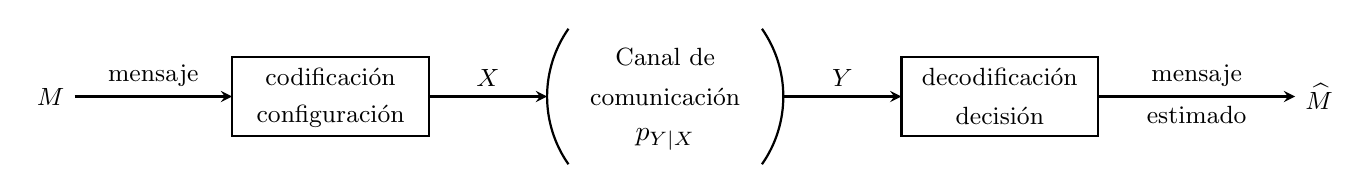
\begin{tikzpicture}
\shorthandoff{>}
%
% Mensaje
\draw[>=stealth,->,thick] (0,0) node[left]{\small $M$} --(2,0);
\draw (1,0) node[above]{\small mensaje};
%
% codificacion
\draw[thick] (2,-.5) rectangle (4.5,.5);
\draw (3.25,.25) node{\small codificaci\'on};
\draw (3.25,-.25) node{\small configuraci\'on};
%
% entrada del canal
\draw[>=stealth,->,thick] (4.5,0)--(6,0);
\draw (5.25,0) node[above]{\small $X$};
%
% Canal de com
\pgfmathsetmacro{\t}{35};
\pgfmathsetmacro{\r}{1.5};
\draw[thick] ({6+\r*(1+cos(180-\t))},{\r*sin(\t)}) arc (180-\t:180+\t:\r);
\draw[thick] ({6+\r*(1+cos(\t))},{-\r*sin(\t)}) arc (-\t:\t:\r);
\draw ({6+\r},.5) node{\small Canal de};
\draw ({6+\r},0) node{\small comunicaci\'on};
\draw ({6+\r},-.55) node{$p_{Y|X}$};
%
% salida
\draw[>=stealth,->,thick] ({6+2*\r},0)--({7.5+2*\r},0);
\draw ({6.75+2*\r},0) node[above]{\small $Y$};
%
% decodificacion/decision
\draw[thick] ({7.5+2*\r},-.5) rectangle ({10+2*\r},.5);
\draw ({8.75+2*\r},.25) node{\small decodificaci\'on};
\draw ({8.75+2*\r},-.25) node{\small decisi\'on};
%
% Mensaje estimado
\draw[>=stealth,->,thick] ({10+2*\r},0)--({12.5+2*\r},0) node[right]{\small $\widehat{M}$};
\draw ({11.25+2*\r},0) node[above]{\small mensaje};
\draw ({11.25+2*\r},0) node[below]{\small estimado};
\end{tikzpicture}
 \end{center}
%
\leyenda{Esquema de comunicaci\'on de Shannon.  En una primera etapa, un mensaje
  $M$ a  transmitir es  c\'odificado (ej.  c\'odigo  binario) o puesto  en forma
  (ej.  s\'imbolos  modulando una  funci\'on para que  sea anal\'ogica y  en una
  banda  de frecuencias  dada).  Sea  $X$ este  mensaje codificado  o  puesto en
  forma.  A la  recepci\'on, se mide $Y$ (ej.  versi\'on  ruidosa de $X$), antes
  de ser decodificado o usado para tomar una decisi\'on, $\widehat{M}$ siendo la
  estimaci\'on de  $M$ (ej.  s\'imbolos estimados  a partir de  $Y$).  Una etapa
  importante es el v\'inculo entre la entrada  $X$ y la salida $Y$ del canal, es
  decir la  cantidad de informaci\'on que  tienen en com\'un.   La capacidad del
  canal es la informaci\'on $I(X;Y)$ m\'axima con respecto a su entrada.}
\label{Fig:SZ:CanalComunicacion}
\end{figure}

\modif{En general, es conviente escribir la informaci\'on mutua bajo la forma \ $I(X;Y)
= H(Y) - H(Y|X)$ \ as\'i que,  fijando ``$X = x$'', la entrop\'ia condicional es
dada por el canal. Lo vamos a ver m\'as adelante en las secciones que siguen.  }

% ================================= canal discreto

\modif{
\subsubseccion{Canal discreto finito}
\label{Sssec:SZ:CanalDiscretoFinito}

En tal  canal el  espacio de estado  de entrada  es discreto finito  \ $\X  = \{
x_1 \,  , \, \ldots \,  , \, x_{|\X|} \}  $ \ tal como  el de salida \  $\Y = \{
y_1 \, , \, \ldots \, , \,  y_{|\Y|} \} $. El canal de transmisi\'on es definido
por la distribuci\'on condicional $p_{Y|X=x}(y)$  es decir, en el caso presente,
por la matriz de probabilidades  condicionales $\Pi \equiv \Pi_{Y|X}$, tambi\'en
conocida  como  {\em  matriz  de transici\'on}~\cite{CovTho06,  Rio07}  (da  las
probabilidades de transici\'on de la entrada  a la salida). En el canal, sacamos
Denotando $H(\Pi_{Y|X})$ vector linea de componente $j$-\'esima la entrop\'ia de
la columna $j$ de la matriz de transici\'on, \ie
%
\[
H(\Pi_{Y|X}) = \begin{bmatrix} H( p_{Y|X = x_1} ) & \cdots &  H( p_{Y|X = x_{|\X|}} ) \end{bmatrix}
\]
%
y de la f\'ormula de probabilidades total, se obtiene la capacidad del canal bajo la forma
%
\[
C = \max_{p_X \in \Simp{|\X|-1}} \left( H\left( \Pi_{Y|X} \, p_X \right) -  H\left( \Pi_{Y|X} \right) p_X \right)
\]

Se notar\'a de que, obviamente de $I(X;Y) = H(X) - H(X|Y) = H(Y) - H(Y|X) \ge 0$
con  las  entrop\'ias condicionales  siendas  positivas,  y entrop\'ias  siendas
m\'axima en el caso de probabilididades uniformes, que
\[
0 \le C \le \min( \log_2 |\X| \, , \, \log_2 |\Y| ) 
\]
%
Adem\'as, de  la propiedad~\ref{Prop:SZ:concavidad} de concavidad  de $H$, queda
claro que,  siendo $\Pi_  H\left( \Pi_{Y|X}  \, p_X  \right)$ sea  c\'oncava con
respecto a  $p_X$.  Ademas,  siendo $H\left( \Pi_{Y|X}  \right) p_X$  lineal con
respecto  a  $p_X$,  aparece  que  $I(X  ;  Y)$  es  c\'oncava  con  respecto  a
$p_X$ \SZ{Ponerlo antes? en las propiedades  de $I$?}. Eso asegura que existe un
m\'aximo y que es \'unico.

Dado  el canal,  hay que  resolver el  problema de  optimizaci\'on, pero  no hay
siepre una  soluci\'on explicitaa de $C$.  Pero en casos particulares,  se puede
simplificar el problema.}


% ---------- canal binario

%\subsubseccion
\paragraph{Canal binario}
%\label{Sssec:SZ:CanalBinario}

Suponiendo  que el  mensaje mandado  en un  canal es  una cadena  de s\'imbolos,
variables   aleatorias  independientes,   se  puede   concentrarse   sobre  cada
s\'imbolo. En este marco, un canal de comunicaci\'on lo m\'as simple es conocido
como  {\it canal  binario}~\cite[Sec.~15]{Sha48}: $X$  es una  variable definida
sobre $\X =  \{ 0 \, , \, 1  \}$; tal tipo de entrada es  natural, pensando a la
codificaci\'on  binaria.  La  salida $Y$  es tambi\'en  definida sobre  $\X$; se
puede imaginar medir y tomar una decisi\'on binaria usando la medida.  Tal canal
es  definido por \modif{la matriz de transici\'on
%
\[
\Pi = \begin{bmatrix} 1 - \varepsilon & \vartheta \\ \varepsilon & 1 - \vartheta \end{bmatrix}
\]
%
(\ie \ $\varepsilon  = P(Y = 1 | X  = 0)$ \ y \  $\vartheta = P(Y = 0 |  X = 1)$
representan  errores   de  comunicaci\'on).}   Tal  canal   es  descrito  figura
Fig.~\ref{Fig:SZ:CanalBinario}-(a).                   La                  figura
Fig.~\ref{Fig:SZ:CanalBinario}-(b) da un esquema ``pr\'actico'' que podr\'ia ser
al origen  de un  tal canal.  Cuando  \ $\varepsilon =  \vartheta$, el  canal es
conocido como {\it canal binario sim\'etrico}.  Cuando \ $\varepsilon = 0$ \ y \
$\vartheta \in (0 \; 1)$, el canal es conocido como {\it canal binario en Z}.

\begin{figure}[h!]
\begin{center} 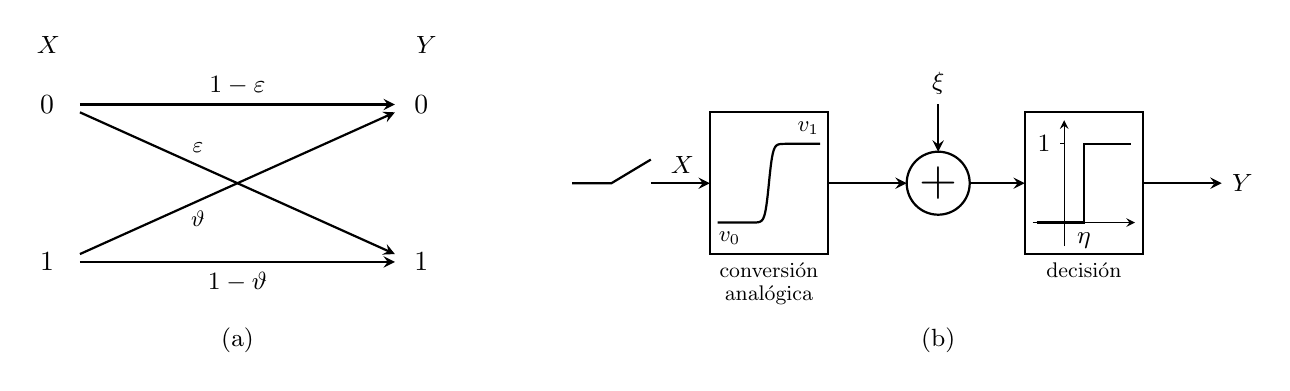
\begin{tikzpicture}
\shorthandoff{>}
%
\begin{scope}
\draw (-.4,1.75) node {\small $X$}; \draw (4.4,1.75) node {\small $Y$};
%
\draw[>=stealth,->,thick] (-.2,1) node[left]{0} (0,1) -- (4,1) node[right]{\ 0};
\draw (2,1) node[above]{\small $1-\varepsilon$};
%
\draw[>=stealth,->,thick] (-.2,-1) node[left]{1} (0,-1) -- (4,-1) node[right]{\ 1};
\draw (2,-1) node[below]{\small $1-\vartheta$};
%
\draw[>=stealth,->,thick] (0,.9)--(4,-.9);
\draw (1.5,.45) node[scale=.9]{\small $\varepsilon$};
%
\draw[>=stealth,->,thick] (0,-.9)--(4,.9);
\draw (1.5,-.45) node[scale=.9]{\small $\vartheta$};
%
\end{scope}
%
\begin{scope}[xshift=7cm]
%
% entrada
\draw[thick] (-.75,0)--(-.25,0)--(.25,.3);
\draw[>=stealth,->,thick] (.25,0)--(1,0);
%\draw[>=stealth,->,thick] (.25,-.5) node[below]{\small $X$} --(.25,.1);
\draw (.65,0) node[above]{\small $X$};
%
% puesta en niveles
\draw[thick] (1,-.9) rectangle (2.5,.9);
\draw (1.25,-.7) node[scale=.9]{\small $v_0$};
\draw (2.25,.7) node[scale=.9]{\small $v_1$};
\draw[thick,domain=-4.5:4.5,samples=100] (1.1,-.5) -- plot ({\x/10+1.75},{.5*tanh(2*\x)}) --(2.4,.5);
\draw (1.75,-.9) node[below,scale=.85]{\small conversi\'on};
\draw (1.75,-1.2) node[below,scale=.85]{\small anal\'ogica};
%
% adicion del ruido
\draw[>=stealth,->,thick] (2.5,0)--(3.5,0);
\draw[thick] (3.9,0) circle (.4);
\draw[>=stealth,->,thick] (3.9,1) node[above]{\small $\xi$} --(3.9,.4);
\draw (3.9,0) node[align=center,scale=1.5]{\large +};
%
% decision
\draw[>=stealth,->,thick] (4.3,0)--(5,0);
\draw[thick] (5,-.9) rectangle (6.5,.9);
\draw[>=stealth,->] (5.1,-.5)--(6.4,-.5);
\draw[>=stealth,->] (5.5,-.8)--(5.5,.8);
\draw[thick] (5.15,-.5)--(5.75,-.5)--(5.75,.5)--(6.35,.5);
\draw (5.75,-.5) node[below]{\small $\eta$};
\draw (5.5,.5)--(5.45,.5) node[left]{\small 1};
\draw (5.75,-.9) node[below,scale=.85]{\small decisi\'on};
%
% salida
\draw[>=stealth,->,thick] (6.5,0)--(7.5,0) node[right]{\small $Y$};
\end{scope}
\draw (2,-2) node {\small (a)};
\draw (10.9,-2) node {\small (b)};
\end{tikzpicture}
 \end{center}
%
\leyenda{(a): Canal binario.  La entrada $X$ definida  sobre $\X = \{ 0  \, , \,
  1\}$ pasa  por este canal  e $Y$  definida sobre $\Y  = \X$ es  recibido. Este
  canal es caracterizado por  las probabilidades de transici\'on $p_{Y|X=x}(y)$.
  (b): Esquema  que puede conducir al  canal binario; una variable  puede ser la
  salida de una puerta l\'ogica, con niveles $v_0$ (nivel bajo, codificando 0) y
  $v_1$  (nivel alto, codificando  1).  Se  puede imaginar  que este  voltaje es
  transmitido por un  canal a\~nandiendo un ruido $\xi$.   En la recepci\'on, se
  toma una  decisi\'on, por ejemplo  0 (resp.  1)  si la medida es  mayor (resp.
  menor)  que  $\eta  =   \frac{v_0  +  v_1}{2}+\Esp[\xi]$.   En  este  ejemplo,
  $\varepsilon$ \ y  \ $\vartheta$ \ van a  ser caracterizados completamente por
  la distribuci\'on  del ruido (y  de los dos  niveles posibles de  la entrada),
  pero no de la distribuci\'on $p_X$.}
\label{Fig:SZ:CanalBinario}
\end{figure}

En este caso, trabajando con bits,  aparece leg\'itimo usar el logaritmo de base
2. Luego, \modif{sean $p_X$ la distribuci\'on de entrada y $p_Y = \Pi \, p_X$ la
de salida,
%
\[
p_X =  \begin{bmatrix} r\\  1-r \end{bmatrix} \qquad  p_Y =  \begin{bmatrix} s\\
1-s  \end{bmatrix}  =  r  (1  - \varepsilon  -  \vartheta)  \begin{bmatrix}  1\\
-1\end{bmatrix} + \begin{bmatrix} \vartheta\\ 1 - \vartheta \end{bmatrix}
%r = P(X = 0),
\]
%
%dando la distribuci\'on  de la entrada.
%La distribuci\'on de la  salida va a ser
%dada a partir de $s = P(Y = 0) = P(Y = 0 | X = 0) P(X = 0) + P(Y = 0 | X
%= 1) P(X = 1)$ es decir
%%
%\[
%s = P(Y  = 0) = \vartheta +  r (1-\varepsilon-\vartheta).
%\]
%
La informaci\'on  mutua,  \ $I_2(X;Y) =  H_2(p_Y) - H_2(\Pi) \, p_X$,}
%=  H_2(Y) -
%H_2(Y|X=0) P(X = 0) + H_2(Y|X=1) P(X = 1)$,
%lo que
toma la expresi\'on
%
\[
I_2(X;Y) = h_2(s) - r h_2(\varepsilon) - (1-r) h_2(\vartheta),
\]
%
donde $h_2(u) = -  u \log_2 u - (1-u) \log_2 (1-u)$  es la entrop\'ia binaria en
bits.  Para calcular la capacidad $C_2$  en bits, hace falta maximizar $I_2$ con
respecto   a   $r$.    Diferenciando    $I_2$   en   $r$,   \ie   $\frac{\partial
  I_2(X;Y)}{\partial  r}  =  \frac{\partial h_2(s)}{\partial  s}  \frac{\partial
  s}{\partial r} - h_2(\varepsilon) + h_2(\vartheta)$, es decir
%
\[
\frac{\partial I_2(X;Y)}{\partial  r} = (1-\varepsilon-\vartheta)  \log_2 \left(
  \frac{1-s}{s} \right) - h_2(\varepsilon) + h_2(\vartheta).
\]
%
\begin{itemize}
\item Claramente,
  %
  \[
  \vartheta = 1-\varepsilon \quad \Rightarrow \quad C_2 = 0.
  \]
  %
  Viene del hecho  que para $\vartheta = 1-\varepsilon$,  de $h_2(\varepsilon) =
  h_2(1-\varepsilon)$ se deduce que $I_2(X;Y)  = 0$ constante. De hecho, en este
  caso, un 0 en la salida puede venir  de un 0 o 1 con probabilidades iguales, y
  lo mismo para  un 1 en la  salida; en otros t\'erminos, la  salida aparece ser
  independiente de la entrada.  Eso se verifica formalmente con $s = \vartheta$,
  dando $p_{Y|X=x}  = p_Y$, dando una  informaci\'on mutua nula,  y entonces una
  capacidad nula.
%
\item Si $\vartheta  \ne 1-\varepsilon$, la derivada de $I_2$  con respecto a $r$
  se anula para $s = s^\opt$ ($r = r^\opt$),
  %
  \[
  s^\opt = \frac{1}{1 +  2^{\frac{h(\varepsilon) - h(\vartheta)}{1 - \varepsilon
        -  \vartheta}}}  \qquad \mbox{siendo}  \qquad  r^\opt  = \frac{s^\opt  -
    \vartheta}{1 - \varepsilon - \vartheta},
  \]
  %
  y  dando   un  extremo   para  $I_2$.   A   continuaci\'on,  $\frac{\partial^2
    I_2}{\partial  r^2} = \frac{(1-\varepsilon-\vartheta)^2}{s  (1-s)} >  0$ (en
  particular para el $s$ ``\'optimo''),  probando que el extremo es un m\'aximo.
  Poniendo  la expresi\'on de  $r^\opt$ en  la formula  de $I_2(X;Y)$,  luego de
  muchos c\'alculos (b\'asicos), se obtiene
  %
  \[
  C_2  =  \log_2\left(  1  +  2^{\frac{h_2(\varepsilon)  -  h_2(\vartheta)}{1  -
        \varepsilon   -  \vartheta}}   \right)  -   \frac{(1  -   \vartheta)  \,
    h_2(\varepsilon)  -   \varepsilon  \,  h_2(\vartheta)}{1   -  \varepsilon  -
    \vartheta}.
  \]
  %
  Cuando  $\vartheta   \to  1-\varepsilon$,  notando   que  $h_2(\varepsilon)  =
  h_2(1-\varepsilon)$ y  tomando el  l\'imite de esta  formula, se  recupera que
  $C_2 \to 0$.
  %
  % ---
  %
  % \newline{\color{red}\bf ¿Interpretacion?  no hay combinacion convexa
  %   $\frac{\varepsilon}{1-\varepsilon-\vartheta}$ siendo del mismo signo que
  %   $\frac{1-\vartheta}{1-\varepsilon-\vartheta}$; nota: $C
  %   = \log_2\left( 1 + 2^{-
  %       \frac{h(1-\vartheta)-h(\varepsilon)}{(1-\vartheta)-\varepsilon}}
  %   \right) + \frac{1}{\varepsilon
  %     (1-\vartheta)} \frac{(1-\vartheta) h(1-\vartheta) - \varepsilon
  %     h(\varepsilon)}{\vartheta - (1-\varepsilon)}$}
\end{itemize}
%
\noindent De  \ $I_2(X;Y) = H_2(Y)  - H_2(Y|X) \le H_2(Y)  \le 1$ bit  \ ($Y$ es
binario, de entrop\'ia m\'axima en el caso uniforme), aparece sin c\'alculos que
%
\[
C_2 \le 1 \: \mbox{bit},
\]
%
\ie  la capacidad  es menor  que 1  bit: para  transmitir informaci\'on  en este
canal, hace falta introducir redundancia en  el mensaje.  Se alcanza \ $C_2 = 1$
bit si, (i) por  un lado $H_2(Y|X) = 0$, es decir  \ $r h_2(\varepsilon) + (1-r)
h_2(\vartheta) = 0$ \ y adem\'as (ii) \ $h_2(s) = 1$.  Estudiando cada caso (ej.
con \ $r = 0$ \ y \ $\vartheta =  0$ \ se satisface (i) pero no (ii) porque \ $s
= 0$), se obtiene que
%
\[
C_2  =  1  \qquad  \Leftrightarrow  \qquad  r =  \frac12  \quad  \mbox{y}  \quad
\varepsilon = \vartheta = \frac{1 \pm 1}{2}.
\]
%
Para  $\varepsilon =  \vartheta =  0$ el  canal es  perfecto, mientras  que para
$\varepsilon =  \vartheta =  1$ el  canal es llamado  {\it canal  volteando}; en
ambos casos, se recupera la entrada (o directamente, o tomando el opuesto) ``sin
perdida''.

La  figura  Fig.~\ref{Fig:SZ:ICanalBinario}  representa la  informaci\'on  mutua
$I(X;Y)$ para unos  canales ($\varepsilon$ y $\vartheta$ dados)  en funci\'on de
$r$.  Se nota que la curva es c\'oncava y tiene un m\'aximo \'unico~\footnote{De
  manera general, de la escritura de $I$ con entrop\'ias condicionales, para $X$
  definido sobre $\X$ e  $Y$ sobre $\Y$, da \ $0 \le C \le  \min( \log |\X| \, ,
  \, \log |\Y|  )$.  \ Adem\'as, $p_{Y|X=x}$  depende solo del canal y  no de la
  entrada, as\'i que  para \ $p_X =  \pi_1 p_{(1)} + \pi_2 p_{(2)}$  \ ($\pi_2 =
  1-\pi_1$) se obtiene \ $p_Y = \pi_1 q_{(1)} + \pi_2 q_{(2)}$ \ con \ $q_{(i)}$
  \ distribuci\'on de la salida corespondiente a una entrada de distribuci\'on \
  $p_{(i)}$.   Ahora, de  $I(X;Y) =  H(Y)-H(Y|X)$, el  segundo  t\'ermino siendo
  dependiente solamente del canal, de la concavidad de $H$ se obtiene de que $I$
  es c\'oncava con respecto a  $p_X$.  A continuaci\'on, $p_X$ parteneciendo a un
  convexo,  $I$ tiene un  m\'aximo que  es \'unico.},  capacidad del  canal.  La
figura  Fig.~\ref{Fig:SZ:CCanalBinario}  representa la  capacidad  del canal  en
funci\'on  de  \   $\varepsilon$  \  y  \  $\vartheta$   as\'i  que  unos  casos
particulares/cortes.

En  el caso  particular  $\varepsilon  = \vartheta$,  conocido  como {\it  canal
  sim\'etico}, la capacidad es
%
\[
C_2 = 1 - h_2(\varepsilon)
\]
%
(alcanzada  con  una entrada  uniforme).   Como visto  en  el  caso general,  la
capacidad vale 1  bit si y solamente si  \ $h_2(\varepsilon) = 0$, \  es decir \
$\varepsilon = 0$ \ o \ $\varepsilon = 1$.  Al rev\'es, la capacidad es m\'inima
cuando $H_2$ est m\'aximo, es decir  para \ $\varepsilon = \vartheta = \frac12$,
\ y  \ $C_2 = 0$  \ (instancia particular  de \ $\vartheta =  1-\varepsilon$). \
$h_2(\varepsilon)$  \  es la  perdida  en bit  para  cada  bit transmitido.   La
capacidad  \  $C_2$   \  en  funci\'on  de  \   $\varepsilon$\  es  dada  figura
Fig.~\ref{Fig:SZ:CCanalBinario}-(b).

En el  caso particular  $\varepsilon = 0$,  conocido como  {\it canal en  Z}, la
capacidad es
%
\[
C_2 = \log_2\left( 1 +  2^{- \frac{h_2(\vartheta)}{1-\vartheta}} \right).
\]
%
Se nota  en este caso tambi\'en  que la capacidad  alcanza 1, su m\'aximo,  si y
solamente  si \  $\vartheta  = 0$  \  (canal perfecto).   Al  rev\'es, cuando  \
$\vartheta  \to 1$,  \  $C \to  0$, \  instancia  particular de  \ $\vartheta  =
1-\varepsilon$.   La capacidad \  $C_2$ \  en funci\'on  de $\vartheta$  es dada
figura Fig.~\ref{Fig:SZ:CCanalBinario}-(c).

%{\bf\color{red} C parecido a la de Shannon caso continuo. Interpretacion?}

\begin{figure}[h!]
%
\begin{center} \begin{tikzpicture}[scale=2]
\shorthandoff{>}
%
%
% ----- Canal general
%
\begin{scope}
\pgfmathsetmacro{\p}{.4};% varepsilon
\pgfmathsetmacro{\q}{.01};% vartheta
%
\pgfmathsetmacro{\dpr}{1-\p-\q};
\pgfmathsetmacro{\hp}{-\p*log2(\p)-(1-\p)*log2(1-\p)};% h(varepsilon)
\pgfmathsetmacro{\hq}{-\q*log2(\q)-(1-\q)*log2(1-\q)};% h(vartheta)
\pgfmathsetmacro{\dh}{\hp-\hq};
%
\pgfmathsetmacro{\bopt}{1/(1+(2^((\hp-\hq)/\dpr)))};% s opt
\pgfmathsetmacro{\aopt}{(\bopt-\q)/\dpr};% r opt
\pgfmathsetmacro{\Capa}{-log2(\bopt)-((1-\q)*\hp-\p*\hq)/\dpr};
%
\draw[>=stealth,->] (-.2,0)--(1.2,0) node[right]{\small $r$};
\draw[>=stealth,->] (0,-.2)--(0,1.2) node[above]{\small $I_2(X;Y)$};
%
\draw[thick,domain=0:1,samples=100] (0,0)-- plot (\x,
{-(\q+\dpr*\x)*log2(\q+\dpr*\x)-(1-\q-\dpr*\x)*log2(1-\q-\dpr*\x)-\x*\hp-(1-\x)*\hq)})
--(1,0);
%
\draw (\aopt,0)--(\aopt,-.05) node[below]{\small $r^\opt$};
\draw (1,0)--(1,-.05) node[below]{\small 1};
\draw (0,\Capa)--(-.05,\Capa) node[left]{\small $C_2$};
\draw (0,1)--(-.05,1) node[left]{\small 1};
\end{scope}
%
%
% ----- Canal simetrico
%
\begin{scope}[xshift=2.5cm]
\pgfmathsetmacro{\p}{.05};
%
\pgfmathsetmacro{\dpr}{1-2*\p};
\pgfmathsetmacro{\hp}{-\p*log2(\p)-(1-\p)*log2(1-\p)};
%
\pgfmathsetmacro{\Capa}{1-\hp};
%
\draw[>=stealth,->] (-.2,0)--(1.2,0) node[right]{\small $r$};
\draw[>=stealth,->] (0,-.2)--(0,1.2) node[above]{\small $I_2(X;Y)$};
%
\draw[thick,domain=0:1,samples=100] (0,0)-- plot (\x,
{-(\p+\dpr*\x)*log2(\p+\dpr*\x)-(1-\p-\dpr*\x)*log2(1-\p-\dpr*\x)-\hp)})
--(1,0);
%
\draw (.5,0)--(.5,-.05) node[below]{\small $r^\opt$};
\draw (1,0)--(1,-.05) node[below]{\small 1};
\draw (0,\Capa)--(-.05,\Capa) node[left]{\small $C_2$};
\draw (0,1)--(-.05,1) node[left]{\small 1};
\end{scope}
%
%
% ----- Canal en Z
%
\begin{scope}[xshift=5cm]
\pgfmathsetmacro{\q}{.3};
%
\pgfmathsetmacro{\dpr}{1-\q};
\pgfmathsetmacro{\hq}{-\q*log2(\q)-(1-\q)*log2(1-\q)};
%
\pgfmathsetmacro{\bopt}{1/(1+(2^(-\hq/\dpr)))};
\pgfmathsetmacro{\aopt}{(\bopt-\q)/\dpr};
\pgfmathsetmacro{\Capa}{-log2(\bopt)};
%
\draw[>=stealth,->] (-.2,0)--(1.2,0) node[right]{\small $r$};
\draw[>=stealth,->] (0,-.2)--(0,1.2) node[above]{\small $I_2(X;Y)$};
%
\draw[thick,domain=0:1,samples=100] (0,0)-- plot (\x,
{-(\q+\dpr*\x)*log2(\q+\dpr*\x)-(1-\q-\dpr*\x)*log2(1-\q-\dpr*\x)-(1-\x)*\hq)})
-- (1,0);
%
\draw (\aopt,0)--(\aopt,-.05) node[below]{\small $r^\opt$};
\draw (1,0)--(1,-.05) node[below]{\small 1};
\draw (0,\Capa)--(-.05,\Capa) node[left]{\small $C_2$};
\draw (0,1)--(-.05,1) node[left]{\small 1};
\end{scope}
\node at  (.5,-.6){\small (a)};
\node at  (3,-.6){\small (b)};
\node at  (5.5,-.6){\small (c)};
\end{tikzpicture}
 \end{center}
%
\leyenda{Informaci\'on mutua  (en bits) entrada-salida \ $I_2(X;Y)$  \ del canal
  binario en funci\'on de \ $r = P(X  = 0)$.  \ (a): \ $\varepsilon = 0.4$ \ y
  \  $\vartheta = 0.01$;  \ (b):  \ $\varepsilon  = \vartheta  = 0.05$  \ (canal
  sim\'etico); \ (c): \  $\varepsilon = 0$ \ y \ $\vartheta  = 0.05$ \ (canal en
  Z).}
%
\label{Fig:SZ:ICanalBinario}
\end{figure}

\

\begin{figure}[h!]
%
\begin{center} \begin{tikzpicture}[scale=2]
\shorthandoff{>}
%
%
% ----- Canal general
%
\begin{scope}
% C(\varepsilon,\vartheta)
%\begin{axis}[colorbar,domain=.01:.99, domain y=.01:.99, samples=10,  samples y=10,
%view={0}{90},  colormap/blackwhite,
%xlabel={\small $\varepsilon$}, ylabel={\small $\vartheta$}, xscale=.27, yscale=.27]
%\addplot3[surf,patch to triangles,shader=interp]
%%{5*sin(deg(2*pi*x))*exp(-4*pi*pi*y)};
%{log2(1+2^((-\x*log2(\x)-(1-\x)*log2(1-\x)+\y*log2(\y)+(1-\y)*log2(1-\y))/(1-\x-\y)))
%+((1-\y)*(\x*log2(\x)+(1-\x)*log2(1-\x))-\x*(\y*log2(\y)+(1-\y)*log2(\y)))/(1-\x-\y)};
%\end{axis}
%\draw(0,0) node{\color{red}\bf A faire};
\draw(1,.75) node{
\includegraphics[width=4cm]{TIKZ_SZ/CapacidadBinaria}};
\draw[>=stealth,->] (-.1,0)--(1.7,0) node[below]{\small $\varepsilon$};
\draw[>=stealth,->] (0,-.1)--(0,1.7) node[left]{\small $\vartheta$};
\draw (1.5,0)--(1.5,-.05) node[below,scale=.8]{\small 1};
\draw (0,1.5)--(-.05,1.5) node[left,scale=.8]{\small 1};
%
\draw (2.075,.02) node[scale=.8]{\small 0};
\draw (2.075,1.48) node[scale=.8]{\small 1};
\end{scope}
%
%
% ----- Canal simetrico
%
\begin{scope}[xshift=3.2cm,scale=1.3]
%
\draw[>=stealth,->] (-.1,0)--(1.2,0) node[right]{\small $\varepsilon$};
\draw[>=stealth,->] (0,-.1)--(0,1.2) node[above]{\small $C_2$};
%
\draw[thick,domain=.01:.99,samples=100] (0,1)-- plot (\x,
{1+\x*log2(\x)+(1-\x)*log2(1-\x)})
--(1,1);
%
\draw (.5,.75) node[scale=.8]{\small $(\vartheta = \varepsilon)$};
\draw (1,0)--(1,-.05) node[below,scale=.8]{\small 1};
\draw (0,1)--(-.05,1) node[left,scale=.8]{\small 1};
\end{scope}
%
%
% ----- Canal en Z
%
\begin{scope}[xshift=6cm,scale=1.3]
%
\draw[>=stealth,->] (-.2,0)--(1.2,0) node[right]{\small $\vartheta$};
\draw[>=stealth,->] (0,-.2)--(0,1.2) node[above]{\small $C_2$};
%
\draw[thick,domain=.01:.99,samples=100] (0,1)-- plot (\x,
{log2(1+2^(log2(1-\x)+(\x/(1-\x))*log2(1-\x)))})
-- (1,0);
%
\draw (.75,.75) node[scale=.8]{\small $(\varepsilon = 0)$};
\draw (1,0)--(1,-.05) node[below,scale=.8]{\small 1};
\draw (0,1)--(-.05,1) node[left,scale=.8]{\small 1};
\end{scope}
\draw (.8,-.4) node {\small (a)};
\draw (3.85,-.4) node {\small (b)};
\draw (6.75,-.4) node {\small (c)};
\end{tikzpicture}
 \end{center}
%
\leyenda{Capacidad  \ $C_2$ \  del canal  binario. \  (a): \  en funci\'on  de \
  $\varepsilon$ \  y \ $\vartheta$. \ (b):  \ en funci\'on de  \ $\varepsilon$ \
  para el canal sim\'etico ($\varepsilon = \vartheta$); \ (c): \ en funci\'on de
  \ $\vartheta$ \ para \ $\varepsilon = 0$ \ (canal en Z).}
%
\label{Fig:SZ:CCanalBinario}
\end{figure}



\modif{
% ---------- canal binario

%\subsubseccion
\paragraph{Canales sim\'etricos}
%\label{Sssec:SZ:CanalBinario}

Se  simplifica  tambi\'en  el  estudio  de capacidad  de  un  canal  cuando  hay
simetr\'ias.  Empezamos  con   las  definiciones  siguentes~\cite{Sha48,  Gal01,
CovTho06}:
%
\begin{definicion}[Canal sim\'etrico en entrada]
Un  canal es  dicho sim\'etrico  en  entrada si  cada  columna de  su matriz  de
transici\'on $\Pi$ se deduce como permutaci\'on de un vector $\pi$, \ie
%
\[
\exists \, \pi \in \Simp{|\Y|-1}, \quad \forall \, j = 1, \ldots , |\X|, \:\:
\exists \, \Sigma_j \in \Perm_{|\Y|}, \:\: p_{Y|x=x_j} = \Sigma_j \, \pi
\]
\end{definicion}

\begin{definicion}[Canal sim\'etrico en salida]
Un  canal es  dicho sim\'etrico  en  salida si  cada  linea de  su matriz  de
transici\'on $\Pi$ se deduce como permutaci\'on de un vector $\widetilde{\pi}$, \ie
%
\[
\exists \, \widetilde{\pi} \in \Simp{|\X|-1}, \quad \forall \, i = 1, \ldots , |\Y|, \:\:
\exists \, \Sigma_i \in \Perm_{|\X|}, \:\: \begin{bmatrix} p_{Y|x=x_1}(y_i) & \cdots &  p_{Y|x=x_{|\X|}}(y_i) \end{bmatrix} = \widetilde{\pi}^t \Sigma_i
\]
\end{definicion}


\begin{definicion}[Canal uniforme en salida]
Un  canal es  dicho uniforme  en  salida si  $\uno$  autovector de  la matriz  de
transici\'on, $\Pi  \uno \propto  \uno$, \ie si  la entrada de  un canal  con esta
transici\'on es uniforme, la salida tambi\'en. Necesariamente, $\Pi \uno = \frac{|\X|}{|\Y|} \, \uno$.

Cuando $|\Y|=|\X|$,  el autovalor  es igual  a uno  y la  matriz est  dicha {\em
bi-estocastica} (recordar que es estochastica, $\uno^t \Pi = \uno^t$).
\end{definicion}


\begin{definicion}[Canal sim\'etrico]
Un canal es dicho {\em  fuertement sim\'etrico}, o simplemente {\em sim\'etrico}
si es a la vez sim\'etrico en entrada y en salida.


Un canal  es dicho {\em  debilmente sim\'etrico} si es  a la vez  sim\'etrico en
entrada y uniforme en salida. De hecho,  se puede ver sencillamente de que si un
canal es sim\'etrico, es obviamente uniforme  en salido (si cada linea se deduce
de una por permutaciones de componentes,  las suma de sus componentes no depende
del \'indice de linea).

\end{definicion}

Cuando  el  canal sigue  una(s)  de  estas  simetrias,  se simplifican  a  veces
drasticamente el calcilo de la capacidad del canal:

\begin{teorema}[Capacidad del canal s\'imetrico en entrada]
Si el  canal de  transmisi\'on es  s\'imetrico en entrada,  con $\pi$  el vector
columna (bajo permutaciones),  la capacidad del canal se alcanza  para la salida
de entrop\'ia m\'axima (con respect a la distribuci\'on de entrada):
%
\[
C = \max_{p_X \in \Simp{|\X|-1}} H(\Pi p_X) - H(\pi)
\]
\end{teorema}
\begin{proof}
El resultat viene  inmediatamente de $H(Y|X) = H(\Pi) \, p_X$,  siendo en este caso
$H(\Pi) = H(\pi) \uno^t$.
\end{proof}


\begin{teorema}[Capacidad del canal debilmente s\'imetrico]
Si el  canal de  transmisi\'on es  debilmente s\'imetrico  con $\pi$  el vector
columna (bajo permutaciones),  la capacidad del canal es dado por
%
\[
C = \log |\Y| - H(\pi)
\]
%
y se alcanza  para la entrada uniforme.
\end{teorema}
\begin{proof}
Siendo     el      canal     sim\'etrico     en     entrada,      tenemos     $C
= \max_{p_X  \in \Simp{|\X|-1}}  H(\Pi p_X)  - H(\pi)$.  Ahora, siendo  el canal
uniforme en salida, si la entrada es uniforme, tambi\'en es la salida, lo que es
de entrop\'ia m\'axima y vale $\log |\Y|$.
\end{proof}

Se puede notar que si el canal es solamente sim\'etrico en entrada, el resultado
no  vale siempre  porque no  siempre se  puede encontrar  una entrada  dando una
salida uniforme.  Un contra-ejemplo es dado  por el canal borrador  de la figura
Fig.~\ref{Fig:SZ:CanalesDiscretos}-(a). En este caso,  la matriz de transici\'on
es dada por
%
\[
\Pi = \begin{bmatrix}
1 - \varepsilon & 0 \\
\varepsilon & \varepsilon \\
0 & 1 - \varepsilon
\end{bmatrix}
\]
%
Claramente, el canal es sim\'etrico en entrada,  pero no es en salida, y tampoco
es uniforme  en salida  si $\varepsilon  \ne \frac13$. De  nuevo, si  perdida de
generalidad, tratando de bits, consideramos  la entrop\'ia en bits (logaritmo de
base  2).    Sencillamente,  $I(X  ;   Y)  =  H(p_Y)  -   h_2(\varepsilon)$  con
$h_2(\varepsilon) =  - \varepsilon  \log_2 \varepsilon -  (1-\varepsilon) \log_2
(1-\varepsilon)$  entrop\'ia  binaria.   Con  la probabilidad  de  entrada  $p_X
= \begin{bmatrix} r & 1-r \end{bmatrix}^t$  se calcula la probabilidad de salida
$p_Y    =     \begin{bmatrix}    r     (1-\varepsilon)    &     \varepsilon    &
(1-r)    \varepsilon   \end{bmatrix}^t$    as\'i    que,   claramente,    cuando
$\varepsilon  \ne \frac13$  no se  puede alcanzar  una distribuci\'on  de salida
uniforme. De hecho, se calcula la entrop\'ia de salida como
%
\[
H(p_Y) = (1 - \varepsilon) h_2(r) + h_2(\varepsilon)
\]
%
Es m\'aximo  cuando la entrada es  uniforme (pero, nuevamente, no  es la salida)
tal que $\max_{p_X} H(p_Y) =  (1-\varepsilon) + h_2(\varepsilon)$ (no vale $\log
3$) dando la capacidad
%
\[
C = 1 - \varepsilon
\]


Un ejemplo particular de canal sim\'etrico es un canal de matriz de transici\'on
dicha {\em circulante}, donde la columna $k+1$ se deduce de la columna $k$ por una permutaci\'on circular de un \'indice
%
\[
\begin{bmatrix}
\pi & \Pi_c \, \pi & \cdots & \Pi_c^{n-1} \, \pi
\end{bmatrix} \qquad \mbox{con} \qquad
%
\pi = \begin{bmatrix} \pi_1 \\ \vdots \\ \pi_n \end{bmatrix}
\quad \mbox{y} \quad
\Pi_c =
%\begin{bmatrix}
%   0   &    1   &    0    & \cdots &   0  \\
%%
%%   0   &    0   & \ddots & \ddots &   0   \\
%%
%\vdots & \vdots & \ddots & \ddots & \vdots\\
%%
%   0   &    0   & \cdots &   0    &   1   \\
%%
%   1   &    0   & \cdots &   0    &   0
%\end{bmatrix}
%=
\sum_{k=1}^n \uno_k \uno_{k+1}^t, \quad \uno_{n+1} \igualc \uno_1
\]
%
o sea, para $n \ge 3$ ($n = 2$ da el canal binario sim\'etrico),
%
$\Pi  =  \begin{bmatrix}
  \pi_1   &   \pi_n  & \pi_{n-1} & \cdots & \pi_2 \\
%
  \pi_2   &   \pi_1  &   \pi_n  & \cdots & \pi_3\\
%
  \pi_3   &   \pi_2  &   \pi_1  & \cdots & \vdots\\
%
 \vdots & \vdots & \vdots & \vdots & \vdots\\
%
  \pi_n   & \pi_{n-1} & \cdots & \pi_2 & \pi_1
\end{bmatrix}
$
%
%(ver notaciones).
}

\

En~\cite{CovTho06,  Rio07}  entre  otros,  se estudian  diversos  otros  canales
discretos, binarios  o con m\'as estados.   Unos son representados  en la figura
Fig.~\ref{Fig:SZ:CanalesDiscretos}     (ver     tambi\'en~\cite{Sha48,    Eli57}
o~\cite{Ari72} para el c\'alculo num\'erico de la capacidad en el caso general).


\begin{figure}[h!]
%
\begin{center} 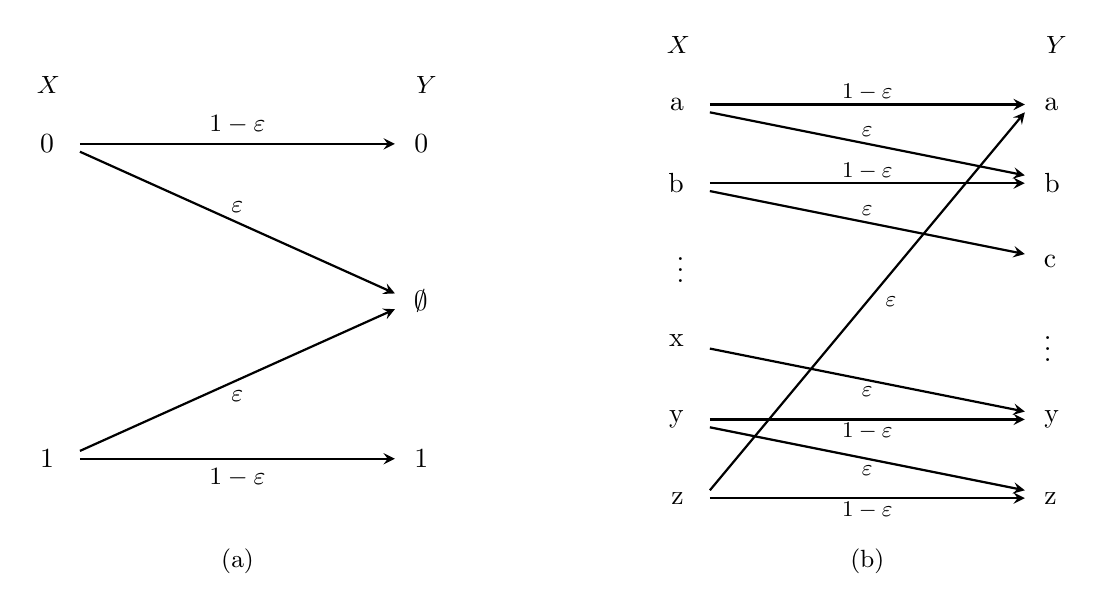
\begin{tikzpicture}
\shorthandoff{>}
%
% Canal borrador
\begin{scope}
\draw (-.4,2.75) node {\small $X$}; \draw (4.4,2.75) node {\small $Y$};
%
\draw[>=stealth,->,thick] (-.2,2) node[left]{0} (0,2) -- (4,2) node[right]{\ 0};
\draw (2,2) node[above]{\small $1-\varepsilon$};
%
\draw[>=stealth,->,thick] (-.2,-2) node[left]{1} (0,-2) -- (4,-2) node[right]{\ 1};
\draw (2,-2) node[below]{\small $1-\varepsilon$};
%
\draw[>=stealth,->,thick] (0,1.9)--(4,.1);
\draw (2,1.2) node{\small $\varepsilon$};
\draw[>=stealth,->,thick] (0,-1.9)--(4,-.1);
\draw (2,-1.2) node{\small $\varepsilon$};
\draw (4,0) node[right]{\ $\emptyset$};
%
\end{scope}
%
% Canal typewriter
\begin{scope}[xshift = 8cm]
\draw (-.4,3.25) node {\small $X$}; \draw (4.4,3.25) node {\small $Y$};
%
% lineas sin error
\draw[>=stealth,->,thick] (-.2,2.5) node[left]{a} (0,2.5) -- (4,2.5) node[right]{\ a};
\draw (2,2.65) node[scale=.9]{\small $1-\varepsilon$};
\draw[>=stealth,->,thick] (-.2,1.5) node[left]{b} (0,1.5) -- (4,1.5) node[right]{\ b};
\draw (2,1.65) node[scale=.9]{\small $1-\varepsilon$};
\draw (-.2,.5) node[left]{$\vdots$}; \draw (4,-.5) node[right]{\ $\vdots$};
\draw[>=stealth,->,thick] (-.2,-1.5) node[left]{y} (0,-1.5) -- (4,-1.5) node[right]{\ y};
\draw (2,-1.65) node[scale=.9]{\small $1-\varepsilon$};
\draw[>=stealth,->,thick] (-.2,-2.5) node[left]{z} (0,-2.5) -- (4,-2.5) node[right]{\ z};
\draw (2,-2.65) node[scale=.9]{\small $1-\varepsilon$};
%
% lineas con el error
\draw[>=stealth,->,thick] (0,2.4) -- (4,1.6);
\draw (2,2.15) node[scale=.9]{\small $\varepsilon$};
\draw[>=stealth,->,thick] (0,1.4) -- (4,.6); \draw (4,.5) node[right]{\ c};
\draw (2,1.15) node[scale=.9]{\small $\varepsilon$};
\draw[>=stealth,->,thick]  (-.2,-.5) node[left]{x} (0,-.6) -- (4,-1.4);
\draw (2,-1.15) node[scale=.9]{\small $\varepsilon$};
\draw[>=stealth,->,thick] (0,-1.6) -- (4,-2.4);
\draw (2,-2.15) node[scale=.9]{\small $\varepsilon$};
\draw[>=stealth,->,thick] (0,-2.4) -- (4,2.4);
\draw (2.3,0) node[scale=.9]{\small $\varepsilon$};
%
\end{scope}
\draw (2,-3.3) node{\small (a)};
\draw (10,-3.3) node{\small (b)};
\end{tikzpicture}
 \end{center}
%
\leyenda{Ejemplos de canales discretos usuales.  (a): canal borrador, donde un 0
  (de probabilidad de ocurrencia $r$) o 1 (de probabilidad de occurrencia $1-r$)
  puede transmitirse  correctamente or  ser borado/perdido  (estado $\emptyset$)
  con una  probabilidad $\varepsilon$.   Se calcula $I_2(X;Y)  = (1-\varepsilon)
  h_2(r)$, dando la capacidad $C_2  = 1-\varepsilon$, alcanzada para una entrada
  uniforme.  (b):  canal tipo  machina de  escribir~\protect\footnotemark, donde
  cada letra  de un ensemble  de $n$  letras (ac\'a con  $n = 26$)  se transmite
  correctamente con una probabilidad $1-\varepsilon$  o a la letra siguiente (de
  manera  c\'iclica) con  una probabilidad  $\varepsilon$. \modif{Este  canal es
  sim\'etrico (de matriz de transici\'on circulante, as\'i que, inmediatamente,
  %De $I_n(X;Y) = H_n(Y) -
  %H_n(Y|X) = H_n(Y)  - h_n(\varepsilon)$ se deduce que $I_n$  es m\'axima si $Y$
  %es uniforme,  lo que es  posible si $X$  es uniforma, dando
  $C = \log_2  n -
  h_2(\varepsilon)$.  Pasando,  para $n  =  2$,  se  recupera el  canal  binario
  sim\'etrico.}.  }
\label{Fig:SZ:CanalesDiscretos}
\end{figure}
%
\footnotetext{Se mencionar\'a de  que en toda esta subsecci\'on,  no se necesita
  de que  $X$ y/o  $Y$ sean  variables aleatorias reales,  \ie pueden  tomar sus
  valores sobre cualquier espacio discreto (por ejemplo de letras).}


% ================================= canal gaussiano

\subseccion{Canal de transmisi\'on continuo gaussiano y su capacidad}
\label{Ssec:SZ:Canalgaussiano}

Un canal de  comunicaci\'on continuo relativamente simple es  conocido como {\it
  canal  gaussiano}~\cite[Sec.~25]{Sha48},~\cite{CovTho06,  Rio07}:  $X$ es  una
variable continua definida  sobre $\X \subset \Rset^d$ y la  salida $Y$ es una
versi\'on ruidosa de $X$, \ie $Y =  X + \xi$ con el ruido $\xi$ independiente de
$X$. En  el canal gaussiano, $\xi  \equiv \N$ es un  vector gaussiano.  Este
canal es tambi\'en definido por  su densidad de probabilidad ``de transici\'on''
$p_{Y|X=x}(y)$,  \ie por  la distribuci\'on  del ruido.   Tal canal  es descrito
figura  Fig.~\ref{Fig:SZ:CanalGaussiano}.   Se  supone  conocida  la  matriz  de
covarianza $\Sigma_\N$ del ruido, y se  nota $\Sigma_X$ la de la entrada. En
pr\'actica, no se puede mandar un mensaje a una potencia tan alta que se quiere,
lo que se traduce por una limitaci\'on
%
\[
\Tr\left(  \Sigma_X  \right) \le  \P,
\]
%
potencia l\'imite permitida por sampleo.

\begin{figure}[h!]
%
\begin{center} 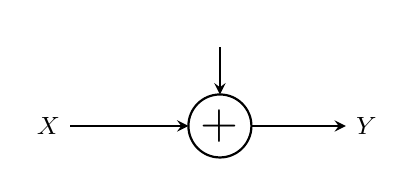
\begin{tikzpicture}
\shorthandoff{>}
%
%
% entrada
\draw[>=stealth,->,thick] (0,0) node[left]{\small $X$} --(1.5,0);
%
% adicion del ruido
\draw[thick] (1.9,0) circle (.4);
\draw[>=stealth,->,thick] (1.9,1) node[above]{\small $\N$} --(1.9,.4);
\draw (1.9,0) node[align=center,scale=1.5]{\large +};
%
% salida
\draw[>=stealth,->,thick] (2.3,0)--(3.5,0) node[right]{\small $Y$};
\end{tikzpicture}
 \end{center}
%
\leyenda{Canal gaussiano. La entrada $X$, modelizada por un vector aleatorio, es
  corrupta aditivamente por un ruido gaussiano $\N$ independiente de $X$. La
  salida es entonces $Y = X + \N$ y el canal es completamente descrito por \
  $p_{Y|X=x}(y)   =   p_\N(y-x)$  \   (obviamente   independiente  de   la
  distribuci\'on de la entrada).}
%
\label{Fig:SZ:CanalGaussiano}
\end{figure}


Por  definici\'on, la informaci\'on  mutua $I(X;Y)$  entrada-salida es  dada por
$I(X;Y) = H(Y) - H(Y|X) = H(Y) - H(\N)$. Maximizar $I(X;Y)$ es equivalente a
maximizar  $H(Y) =  H(X  + \N)$  sujeto  a $\Tr\left(  \Sigma_X \right)  \le
\P$. Fijando  un $\Sigma_X$, la  propiedad~\ref{Prop:SZ:cotamaximagaussiana} \ de
la entrop\'ia diferencial implica que $H(Y)$  sea m\'axima si y solamente si $Y$
es gaussiana,  es decir  si y solamente  si $X$  est gaussiana, dando  $I(X;Y) =
\frac12  \log \left|  \Sigma_X +  \Sigma_\N  \right| -  \frac12 \log  \left|
  \Sigma_\N \right|$. Tomando en cuenta  el l\'imite de potencia, hace falta
maximizar $\left| \Sigma_X  + \Sigma_\N \right|$ sujeto a  $\Tr \Sigma_X \le
\P$ \  y \ $\Sigma_X  \ge 0$ sim\'etica  lo que no  es trivial.  Se  encuentra el
enfoque  permitiendo solucionar  el problema  en~\cite[Sec.~9.4]{CovTho06}.  Sea
$U$, matriz  ortogonal ($U U^t =  U^t U = I$)  de los autovectores  de la matriz
$\Sigma_\N  \ge 0$  sim\'etica~\footnote{Se  recordar\'a de  que  $A \ge  0$
  significa que $A$  es definida no negativa.}, de  columnas $u_i$ ordenadas tal
que los autovalores corespondientes  $\lambda^\N_i$ sean en orden creciente,
\ie
%
\[
\Sigma_\N  =  U  \Diag\left(  \begin{bmatrix} \lambda^\N_1  &  \cdots  &
    \lambda^\N_d \end{bmatrix}^t \right) U^t  \qquad \mbox{con} \qquad 0 \le
\lambda^\N_1 \le \cdots \le \lambda^\N_d,
\]
%
donde $\Diag$ es la matriz diagonal teniendo los $\lambda_i$ en su diagonal (ver
notaciones).   Sea \ $R_X  = U^t  \Sigma_X U$.   Es sencillo  ver que  \ $\left|
  \Sigma_X + \Sigma_\N \right| = \left| R_X + \Lambda_\N \right|$ \ (de $|A B| =
|A| \,  |B|$) \ y  que \ $\Tr \Sigma_X  = \Tr R_X$  (de $\Tr(A B) =  \Tr(B A)$).
Entonces, el problema se reduce a  maximizar \ $\left| R_X + \Lambda_\N \right|$
\ sujeto a \  $\Tr R_X \le \P$ \ y \ $R_X \ge  0$ sim\'etica.  La desigualdad de
Hadamard ya evocada da \ $\left| R_X + \Lambda_\N \right| \le \prod_i \left( R_X
  +  \Lambda_\N  \right)_{i,i}  =  \prod_i  \left( \left(  R_X  \right)_{i,i}  +
  \lambda^\N_i   \right)$   \  donde   $(\cdot)_{i,i}$   denota  el   componente
$(i,i)$-\'esima  de la  matriz, con  igualdad si  y solamente  si \  $R_X$  \ es
diagonal: para maximizar \ $\left| R_X + \Lambda_\N \right|$, \ $R_X$ \ debe ser
entonces  diagonal (dada  una  diagonal, se  alcanza  el m\'aximo  si los  otros
t\'erminos son  nulos).  Es decir  que la base  que diagonaliza \  $\Sigma_\N$ \
debe  diagonalizar  tambi\'en $\Sigma_X$.   Sean  ahora  \  $\lambda^X_i$ \  los
t\'erminos  diagonales   de  $R_X$:  queda  que  maximizar   \  $\prod_i  \left(
  \lambda^X_i + \lambda^\N_i \right)$ \ sujeto a $\sum_i \lambda^X_i \le \P$ \ y
\ $\lambda^X_i \ge 0$.  Este problema de optimizaci\'on sujeto a una desigualdad
se  resuelva  con el  enfoque  de  Karush-Kuhn-Tucker~\footnote{Se introduce  el
  factor de Lagrange y se  maximiza \ $\prod_i \left( \lambda^X_i + \lambda^\N_i
  \right) +  \eta \sum_i \lambda^X_i$.  Eso  da \ $\lambda^X_i  + \lambda^\N_i =
  \lambda$ \  constante si $\lambda$ es  tal que se satisfaga  la positividad de
  $\lambda^X_i$, y $\lambda^X_i = 0$  sino.  En otras palabras, \ $\lambda^X_i =
  \left( \lambda -  \lambda^\N_i \right)_+$ con $\lambda$ el  factor de Lagrande
  despu\'es  de una  reescritura.  Queda  que maximizar  los  $\lambda^X_i$ para
  maximizar $\left| R_X + \Lambda_\N \right|$, es decir tomar $\lambda$ lo m\'as
  grande  que se  puede, pero  satisfaciendo  $\sum_i \lambda^X_i  \le \P$,  \ie
  alcanzando  la   igualdad.\label{Foot:SZ:KKT}}  (KKT)~\cite{Mil00,  CamMar09},
dando  \  $\lambda^X_i  = \left(  \lambda  -  \lambda^\N_i  \right)_+$ \  con  \
$(\cdot)_+ = \max(\cdot,0)$ \ y \ $\lambda$ \ tal que \ $\sum_i \left( \lambda -
  \lambda^\N_i \right)_+ = \P$.  En conclusi\'on, la capacidad es dada por
%
\begin{eqnarray*}
C =  \frac12 \log \left(  \frac{\left| \Sigma_\N +  \Sigma_X \right|}{\left|
      \Sigma_\N  \right|}  \right)  & \quad \mbox{con} \quad &  \Sigma_X  =  U
\Diag\left( \begin{bmatrix} \left(\lambda - \lambda^\N_1\right)_+ & \cdots & \left(\lambda -
    \lambda^\N_d \right)_+ \end{bmatrix}^t \right) U^t,\\[2.5mm]
%
& &  \lambda \ \mbox{ tal que } \:
\sum_i \left(\lambda - \lambda^\N_i \right)_+ = \P
\end{eqnarray*}
%
alcanzada por $X$ gaussiano de matriz de covarianza $\Sigma_X$ as\'i construida.

La  \'ultima condici\'on  se resuelva  a  trav\'es de  lo que  es conocido  como
``llenado   de   agua''   (water-filling   en   ingl\'es),   illustrado   figura
Fig.~\ref{Fig:SZ:WaterFilling}.   El  principio  es  parecido  a  tener  niveles
$\lambda^\N_i$  representando  las  potencias  del  ruido (en  la  base  que
diagonaliza la  matriz de covarianza), y  de ``llenar con agua''  hasta un nivel
$\lambda$ tal que el ``volumen''  a\~nadido vale $\P$; en cada $\lambda^\N_i$
se ha a\~nadido el $\lambda^X_i$~\cite[Sec.~9.4]{CovTho06}.

\begin{figure}[h!]
%
\begin{center} \begin{tikzpicture}
\shorthandoff{>}
%
% Filling
\filldraw[fill=gray!30] (3,2)--(3,1.5)--(2,1.5)--(2,1)--(1,1)--(1,.75)--(0,.75)--(0,2);
%
%Axes
\draw[>=stealth,->] (-.1,0)--(6,0);% node[right]{\small $i$};
\draw[>=stealth,->] (0,-.1)--(0,3);
\draw (0,.85) node[left]{\rotatebox{90}{\footnotesize Potencias}};
%
% neveles de ruido
\draw[thick] (0,.75)--(1,.75)--(1,0); \draw(.5,.375) node{\small $\lambda^\N_1$};
\draw[thick] (1,.75)--(1,1)--(2,1)--(2,0); \draw(1.5,.5) node{\small $\lambda^\N_2$};
\draw[thick] (2,1)--(2,1.5)--(3,1.5)--(3,0); \draw(2.5,.75) node{\small $\lambda^\N_3$};
\draw[thick] (3,1.5)--(3,2.25)--(4,2.25)--(4,0); \draw(3.5,1.125) node{\small $\lambda^\N_4$};
\draw[thick] (4,2.25)--(4,2.75)--(5,2.75)--(5,0); \draw(4.5,1.375) node{\small $\lambda^\N_5$};
\draw[thick] (5.5,1.25) node{\bf $\cdots$};
%
% nivel lambda y potencias de los X
\draw[thick] (0,2) node[left]{\small $\lambda$}--(3,2);
\draw (1,.75)--(1,2); \draw (.5,1.375) node{\small $\lambda^X_1$};
\draw (2,1)--(2,2); \draw (1.5,1.5) node{\small $\lambda^X_2$};
\draw (3,1.5)--(3,2); \draw (2.5,1.75) node{\small $\lambda^X_3$};
\end{tikzpicture}
 \end{center}
%
\leyenda{Principio   del  ``water-filling''   para  obtener   los  $\lambda^X_i$
  satisfaciendo  el v\'inculo de  potencia l\'imite  y permitiendo  de construir
  $\Sigma_X$ a partir  de la matriz diagonal de los $\lambda^X_i$  y la base que
  diagonaliza  la  covarianza  $\Sigma_\N$  del  ruido.  La  zona  en  grise
  representa esquem\'aticamente $\P$.}
%
\label{Fig:SZ:WaterFilling}
\end{figure}

En   el   caso   escalar,   se   obtiene
%
\[
C = \frac12 \log\left( 1 + \frac{\P}{\sigma_\N^2} \right),
\]
%
donde     $\frac{\P}{\sigma_\N^2}$     es     conocido    como     relaci\'on
se\~nale-ruido~\footnote{Esta formula es muy  parecida a la de Shannon, Laplume,
  o Clavier~\cite{Sha48,  Lap48, Cla48} (ver tambi\'en~\cite[Sec.~9.3]{CovTho06}
  o~\cite[Sec.~11.2]{Rio07}).   De hecho,  si se  considera  s\'imbolos mandados
  durante  $T$ segundos  cada  uno (s\'imbolos  puestos  en forma  para dar  una
  se\~nal anal\'ogica) usando una banda  de transmisi\'on $B$, por el teorema de
  Nyquist $B = \frac{1}{2 T}$ (caso l\'imite). Si el ruido es blanco en la banda
  $B$, de densidad espectral de potencia por unidad de frecuencia igual a $N_0$,
  para  un  s\'imbolo  la  relaci\'on  se\~nal-ruido  se  escribe  $\frac{\P}{N_0
    B}$. Adem\'as,  se calcula en general  la capacidad por unidad  de tiempo es
  decir la capacidad  por s\'imbolo divido por  $T = \frac{1}{2 B}$, \ie  $C = B
  \log\left( 1 +  \frac{\P}{N_0 B} \right)$ por segundos,  lo que es precisamente
  la capacidad calculdada por Shannon.  Esta es a veces conocida como formula de
  Shannon-Hartley.}

En~\cite{CovTho06,  Rio07}  por ejemplo,  se  dan  otros  ejemplos de  canal  de
comunicaci\'on   en   el   contexto   continuo   (entrada   $X_t$   siendo   una
se\~nal/proceso, canal filtrando, canal con retroacci\'on (o feedback), etc.).

% ================================= codificacion

\subseccion{Codificaci\'on entr\'opica sin perdida}
\label{Ssec:SZ:Codificacion}

El  problema  de  codificaci\'on  de  fuente  puede  presentarse  de  la  manera
siguiente~\cite[cap.~5]{CovTho06}  o   \cite[cap.~13]{Rio07}.   Sea  un  proceso
aleatorio $\left\{  X_t \right\}_{t \in \Zset}$,  supuesto estacionario, llamado
{\it  fuente}, donde  los $X_t$  toman sus  valores sobre  un  alfabeto discreto
finito no necesariamente real ($X$ puede tomar cualquier etiqueta)
%
\[
\X = \{ x_1 \, , \, \ldots \, , \, x_\alpha \} \qquad \mbox{alfabeto fuente},
\]
%
de  distribuci\'on  $p_X$.   A  cada posible  secuencia~\footnote{Por  abuso  de
  escritura una  cadena de  $n$ s\'imbolos puede  ser vista como  una $n$-upla.}
$s_1  \cdots s_n \in  \X^n$ de  letras de  $\X$, se  quiere asignar  un c\'odigo
$c(s_1 \cdots s_n)$ de letras de un alfabeto discreto finito,
%
\[
\C = \{ \cod_1 \, , \, \ldots \, , \, \cod_d \} \qquad \mbox{ alfabeto c\'odigo}.
\]
%
El c\'odigo es dicho {\it $d$-ario}.   Por ejemplo, se puede asignar un c\'odigo
$c(x_i)  = \cod_{i,1}  \cdots  \cod_{i,l_i} \in  \C^{l_i}$  a cada  s\'imbolo $x_i$,
c\'odigo llamado  {\it palabras c\'odigos}, y  a secuencias $s_1  \cdots s_n$ la
concatenaci\'on de las palabras  c\'odigos correspondiente a cada s\'imbolo, \ie
el  c\'odigo $c(s_1) \cdots  c(s_n)$.  En  el sistema  Moorse por  ejemplo, $\C$
consiste en  un punto,  una barra,  una espacio entre  letras, un  espacio entre
palabras.  En una computadora en general todo  se codifica en bits $\C = \{ 0 \,
, \, 1\}$.  M\'as formalmente, sean
%
\[
\F_\X   =   \bigcup_{k=0}^{\infty}  \X^k   \qquad   \mbox{y}   \qquad  \F_\C   =
\bigcup_{k=0}^{\infty} \C^k,
\]
%
uni\'on  de  secuencias de  $k$  letras de  $\X$  y  $\C$ respectivamente.
%
\modif{
\begin{definicion}[Codificaci\'on de  fuente]
\label{Def:SZ:CodificationDeFuente}
Una
codificaci\'on de  fuente consiste  en una  funci\'on de \  $\F_\X$ \  dentro de
$\F_\C$. En lo  que sigue, nos concentramos en  c\'odigos definidos para bloques
de s\'imbolos de tama\~no $m \ge 1$:
%
\[
\begin{array}{lccl}
c_m: & \X^m & \rightarrow & F_\C\\[.5mm]
%
& x & \mapsto & c_m(x) \in \C^{l_{c_m}(x)}
\end{array},
\]
%
donde $l_{c_m}(x) \in \Nset_0$ es el  {\it largo} de la palabra c\'odigo $c_m(x)$,
y
%
\[
\forall \,  n \ge 1,  \quad \forall  \, s_1 \cdots  s_n \in \big(  \X^m \big)^n,
\quad c_m(s_1 \cdots s_n) \equiv c_m(s_1) \cdots c_m(s_n),
\]
%
lo  que  es  llamado {\it  extensi\'on  del  c\'odigo}.   En  lo que  sigue,  se
escribir\'a $c \equiv c_1$.
\end{definicion}
}

Una manera ingenua de codificar consiste a apoyarse sobre la descomposici\'on de
base \ $d$  \ de un entero, \ie para  $1 \le i \le \alpha$  se puede escribir de
manera \'unica \ $i-1 = (i_0-1) + (i_1-1) d + \cdots + (i_K-1) d^K$ \ donde \ $K
= \Big\lceil \log_d |\X| \Big\rceil$ \ y \ $1 \le i_k \le \alpha$.  Entonces, se
puede asignar la palabra c\'odigo \ $c(x_i) = \cod_{i_0} \cdots \cod_{i_k}$ \ al
s\'imbolo  $x_i$.  Haciendo  eso, cada  palabra c\'odigo  tieno el  mismo largo.
Pero, es m\'as  econ\'omico hacer una codificaci\'on dicha  de largos variables,
teniendo   en  cuenta  las   probabilidades  de   aparici\'on  de   cada  $x_i$.
Implicitamente, es la idea del c\'odigo  de Moorse, que asigna un punto o series
de puntos o  c\'odigo peque\~no a las letras muy frecuentes  (ej.  un punto para
el `e',  dos puntos para el  `i', etc.), y  barras o combinaciones largas  a las
letras que son raras (ej. bara-bara-punto-bara para el `q' o cinco baras para el
`0').  Dicho de  otra manera, el c\'odigo ingenuo  ser\'ia ``eficaz'' para $x_i$
apareciendo con las mismas frecuencias/probabilidades.

En los c\'odigos de largos variables (incluyendo el c\'odigo ingenuo), volviendo
a  $c_m$, existen  varios tipos  de  c\'odigos.  Un  c\'odigo es  dicho {\it  no
  singular} si $c_m$  es inyectiva: a cada $x \in  \X^m$ corresponde una palabra
c\'odigo \'unica. Esta propiedad es un requisito que parece obvio querer para un
c\'odigo.  Pero  no es suficiente  para poder decodificar un  mensaje, compuesta
por una  secuencia de palabras  c\'odigo.  Lo importante  en este caso  es poder
decodificar  la   secuencia  sin  ambig\"uedad:  un  c\'odigo   est  dicho  {\it
  descifrable} o {\it  a decodificaci\'on \'unica} (o sin  perdida) si todas las
extensiones son no singulares.
%
\begin{ejemplo}[C\'odigo no singular, pero no decifrable]
\label{Ej:SZ:CodigoNoSingularDecifrable}
%
Sean \ $\X = \{ \aleph \, , \, \beth \, , \, \gimel \, , \, \daleth \}$, \ $\C =
\{0 \, , \, 1  \}$ \ y \ $c(\aleph) = 0, \: c(\beth) =  00, \: c(\gimel) = 1, \:
c(\daleth) =  01$ ($m = 1$).  El  c\'odigo es no singular,  pero no descifrable.
La  secuencia  $0010$  puede  provenir  de $\aleph\aleph\gimel\aleph$,  \  de  \
$\aleph\daleth\aleph$ \ o de \ $\beth\gimel\aleph$.
\end{ejemplo}
%
Obviamente,  se  requiere  en  general  de  un  c\'odigo  que  sea  descifrable.
Frecuentemente,  se requiere tambi\'en  poder decodificar  sobre la  marcha, sin
esperar de medir toda la secuencia  codificada: es lo que se llama {\it c\'odigo
  instantaneo}.
%
\begin{ejemplo}[C\'odigo decifrable, pero no instantaneo]
\label{Ej:SZ:CodigoDcifrableNoInstantaneo}
%
  Sea el  c\'odigo $c(\aleph)  = 00,  \: c(\beth) =  10, \:  c(\gimel) =  11, \:
  c(\daleth)  =  110$.  Este  c\'odigo  es  descifrable,  pero  no  instantaneo.
  Considera la secuencia  $0011011$ y marcha sobre ella.  $0$  no es una palabra
  c\'odigo; $00$  es y sin  ambig\"uedad proviene de  un $\aleph$ (no  hay otras
  palabras  empezando por $00$);  luego $1$  no es  una palabra,  y $11$  es una
  palabra  c\'odigo,  pero se  necesita  adelantar para  saber  si  viene de  un
  $\gimel$ o de un $\daleth$; la  letra siguiente siendo un $0$, todav\'ia no se
  puede concluir si $110$ vino de  $\gimel$ y alg\'o o $\daleth$.  Al final, con
  $1101$, se  sabe que se tuvimos  un $\daleth$ porque  ninguna palabra c\'odigo
  empieza por $01$.   Al final, sin ambig\"uedad el  antecedente de la secuencia
  binaria era  $\aleph\daleth\gimel$.  Pero se necesit\'o marchar  sobre toda la
  secuencia antes de decodificar.
\end{ejemplo}
%
Obviamente,  un c\'odigo  instantaneo es  tal  que ninguna  palabra c\'odigo  es
prefijo de una otra, \ie si $c_m(x)$ es una palabra c\'odigo, las otras palabras
c\'odigo no  pueden empezar  con $c_m(x)$; el  c\'odigo es tambi\'en  dicho {\it
  libre  de  prefijo}.   Estas   distinciones  estan  ilustradas  en  la  figura
Fig.~\ref{Fig:SZ:ClasesCodigos} (ver~\cite[cap.~5]{CovTho06}).

\begin{figure}[h!]
%
\begin{center} 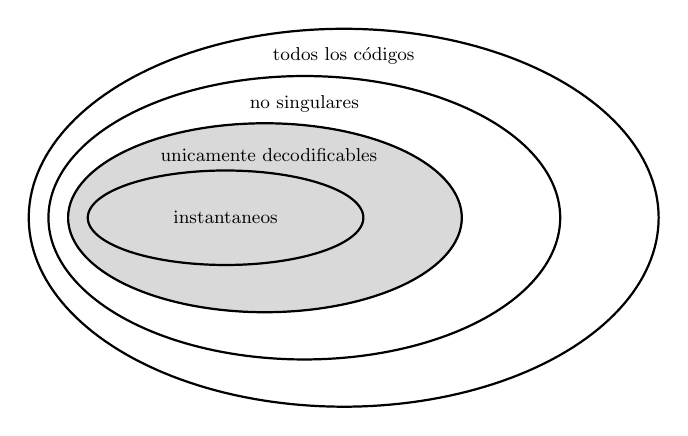
\begin{tikzpicture}
\shorthandoff{>}
\filldraw[fill=gray!30,domain=0:360, samples=200] plot ({2.5*cos(\x)+.5},{1.2*sin(\x)});
%%%%
\draw[thick,domain=0:360, samples=200] plot ({1.75*cos(\x)},{.6*sin(\x)});
\node[scale=.75] at (0,0){\small instantaneos};
%
\draw[thick,domain=0:360, samples=200] plot ({2.5*cos(\x)+.5},{1.2*sin(\x)});
\node[scale=.75] at (.55,.8){\small  unicamente decodificables};
%
\draw[thick,domain=0:360, samples=200] plot ({3.25*cos(\x)+1},{1.8*sin(\x)});
\node[scale=.75] at (1,1.45){\small no singulares};
%
\draw[thick,domain=0:360, samples=200] plot ({4*cos(\x)+1.5},{2.4*sin(\x)});
\node[scale=.75] at (1.5,2.05){\small todos los c\'odigos};
\end{tikzpicture}
 \end{center}
%
\leyenda{Clases  de c\'odigos.   Los  c\'odigos  contienen la  clase  de los  no
  singulares.  La misma  contiene la clase de los  c\'odigos descifrables.  Ella
  contiene los  c\'odigos instantaneos.  En  grise se representan las  clases de
  c\'odigos sin perdida a lo cuales se dedica esta secci\'on.}
%
\label{Fig:SZ:ClasesCodigos}
\end{figure}

Adem\'as  de   la  decodificaci\'on  sin   ambig\"uedad,  una  caracterizaci\'on
importante del  c\'odigo es la  taza de codificaci\'on~\footnote{En~\cite{Rio07}
  por  ejemplo, se  define esta  taza suponiendo  que cada  secuencia  fuente es
  codificada por el  mismo n\'umero de bits. La taza es  entonces el n\'umero de
  bits por s\'imbolo.}:
%
\modif{
\begin{definicion}[Taza de codificaci\'on y largo promedio]
\label{Def:SZ:TazaDeCodificacionLargoPromedio}
%
Sea $X$ una  secuencia de $m \ge  1$ variables $X_t$ tomado su  valores sobre el
alfabeto $\X$.  Sea $c_m$ un c\'odigo  de fuente con $l_{c_m}(x)$  los largos de
los c\'odigos $c_m(x),  \: x \in \X^m$. La taza  de codificaci\'on est definida
por
%
\[
R_{c_m} = \frac{\displaystyle \log_d \left( \sum_{x \in \X^m} l_{c_m}(x) \modif{p_X(x)} \right)}{m},
\]
%
El argumento  del logaritmo (de  base adecuada al cardenal  de $\C$) es  el {\it
largo promedio} del c\'odigo:
%
\[
L(c_m) = \sum_{x \in \X^m} l_{c_m}(x) \modif{p_X(x)}
\]
%
\modif{con $p_X(x) =  P(X = x)$.}
\end{definicion}
%donde $X$  representa una  secuencia de $m$  variables $X_t$.  El  argumento del
%logaritmo (de base adecuada al cardenal  de $\C$) es el {\it largo promedio} del
%c\'odigo.
Por ejemplo,  para $d = 2$, $R_{c_m}$ es el  n\'umero de bits promedio
del c\'odigo por s\'imbolo.

Antes de ir  m\'as adelante, en esta  secci\'on, ya se puede  notar el v\'inculo
entre la codificaci\'on y la noci\'on de entrop\'ia. M\'as precisamente, aparece
que el largo promedio de un c\'odigo es nada m\'as que una entrop\'ia cruzada:
%
\begin{lema}[Largo promedio y entrop\'ia cruzada]
%
Sea $X$ una  secuencia de $m \ge  1$ variables $X_t$ tomado su  valores sobre el
alfabeto $\X$.  Sea  $c_m$ un c\'odigo de fuente con  $l_{c_m}(x)$ los largos de
los c\'odigos $c_m(x) \in F_{\C}, \: x \in \X^m$. Sean $p_X$ la distrbuci\'on de
$X$ y la distribuci\'on
%
\[
q_{c_m}(x) = \frac{d^{-l_{c_m}(x)}}{\sum_{y \in \X^m} d^{-l_{c_m}(y)}}
\]
%
Entonces, el largo promedio se escribe usando una entrop\'ia cruzada
%
\[
L(c_m) = H_{\mathrm{cruz},d}\left( p_X \| q_{c_m} \right) - \log_d\left( \sum_{x \in \X^m} d^{-l_{c_m}(x)} \right)
\]
%
entrop\'ia cruzada de la distribuci\'on de la fuente con referencia \ $q_{c_m}$:
es el promedio de la ingnorancia  de $q_{c_m}$ (distribuci\'on de largo promedio
m\'inimo como lo veremos) sobre la distribuci\'on de la fuente.
\end{lema}
%
\begin{proof}
El resultado sale inmediatamente de la  definici\'on del largo promedio donde se
usa      $l_{c_m}(x)      =      -     \log_d\left(      q_{c_m}(x)      \right)
- \log_d\left( \sum_{y \in \X^m} d^{-l_{c_m}(y)} \right)$.
\end{proof}

Este  resultado da  un  primera justificaci\'on  del hecho  de  que hablamos  en
general de {\em codificaci\'on entropica}.
}

En general,  se quiere minimizar $R_{c_m}$  (compresar el mensaje  a mandar), lo
que puede  ser contradictorio con la  necesidad de a\~nadir  redundancia para no
perder  informaci\'on   durante  una  transmisi\'on.   En  lo   que  sigue,  nos
concentramos en  el problema  de compresi\'on,  sin tener en  cuenta el  paso de
transmisi\'on  de  mensajes codificados  en  un  canal.   Minimizar la  taza  es
equivalente a minimizar el largo  promedio. Adem\'as, se puede focalisarse en $m
= 1$; todo se extiende sencillamente a $m > 1$.

La meta de  la compresi\'on es entonces construir  un c\'odigo $c$, descifrable,
que minimizar el largo promedio $L(c)$.
%
%\[
%L(c) = \sum_{x \in \X} p_X(x) \, l(x).
%\]
%
Antes de ir  m\'as adelante, hace falta traducir en  ecuaci\'on el v\'inculo que
$c$    sea    descifrable.    Eso    es    dado    por    la   desigualdad    de
Kraft-McMillan~~\cite{Kra49,   McM56,   Kar61}~\footnote{Esta  desigualdad   fue
  probabada  por  L.  G.   Kraft  para c\'odigos  instantaneos  en  su tesis  de
  maestria~\cite{Kra49}.  Luego, fue extendida  a los c\'odigos descifrables por
  B.  McMillan~\cite{McM56} (en  una nota de pie de pagina  de su papel, atribua
  esta  observaci\'on a J.   L.  Doob  hecha oralemente  durante una  escuela de
  verano en Ann Arbor, MI en agosto 1955).}
%
\begin{teorema}[Desigualdad de Kraft-McMillan]
\label{Teo:SZ:KraftMcMillan}
%
  Los largos  $l_c(x)$ de las palabras  c\'odigo de un  c\'odigo $c$ descifrable
  deben satisfacer la desigualdad
  %
  \[
  \sum_{x \in \X} d^{-l_c(x)} \le 1.
  \]
  %
  Rec\'iprocamente,  para cada  conjunto de  enteros $\{  \ell_x \}_{x  \in \X}$
  satisfaciendo  esta   desigualdad,  es   posible  de  construir   un  c\'odigo
  descifrable con $l_c(x) = \ell_x$.
\end{teorema}
%
\begin{proof}
  Para cualquier $k \ge 1$ y cualquiera  cadena $s = s_1 \cdots s_k \in \X^k$, la
  extensi\'on  del  c\'odigo,  $c_k(s_1  \cdots  s_k) =  c(s_1)  \cdots  c(s_k)$
  satisface $l_{c_k}(s) = \sum_{i=1}^k l_c(s_i)$. Entonces
  %
  \[
  \left(  \sum_{x  \in \X}  d^{-l_c(x)}  \right)^k \:  =  \:  \sum_{\bar{x} \in  \X^k}
  d^{-l_{c_k}(\bar{x})} \: = \: \sum_{m=1}^{k \, l_c^{\max}} \#(m) \, d^{-m},
  \]
  %
  re-escribiendo  la segunda  suma, agrupando  los t\'erminos  de  mismo largos,
  donde $\#(m)$  es el n\'umero de c\'odicos  de $\X^k$ teniendo el  largo $m$ y
  $l_c^{\max}  =  \max_{x  \in  \X}  l_c(x)$  es el  largo  mayor.   $c$  siendo
  descifrable,  $c_k$ debe  ser inyectiva,  imponiendo $\#(m)  \le d^m$  (no hay
  m\'as palabras de  largo $m$ que el cardenal  de $\C^m$), dando inmediatemente
  que necesariamente
  %
  \[
  \forall \,  k \in \Nset_0, \quad \sum_{x  \in \X} d^{-l_c(x)} \le  \left( k \,
    l_c^{\max}  \right)^{\frac1k} \quad  \Leftrightarrow \quad  \sum_{x  \in \X}
  d^{-l_c(x)} \le \min_{k \in \Nset_0} \left( k \, l_c^{\max} \right)^{\frac1k}.
  \]
  %
  Un estudio r\'apido de \  $u \mapsto \left( u \, l_c^{\max} \right)^{\frac1u}$
  \ para \  $u \ge 1$ \ y  teniendo en cuenta de que $l_c^{\max}  \le 1$ permite
  concluir  que el  m\'inimo  es igual  a  1, terminando  la  parte directa  del
  teorema.

  Rec\'iprocamente, sea  \ $\{ \ell_x  \}_{x \in \X}$  \ un conjunto  de enteros
  satisfaciendo la  desigualdad de Kraft-McMillan.  Se puede  agrupar los largos
  iguales y  clasificarlos. Sea \ $n_\ell$ \  los n\'umeros de largos  igual a \
  $\ell =  1 , \ldots  , \ell^{\max} \le  \alpha$.  Consideramos ahora  un arbol
  empezando con una ra\'iz, correspondiente a un largo $0$, que se divide en $d$
  ramas, correspondiente a los largos iguales  a $1$; a cada nudo se asocian las
  letras \  $\cod_1, \ldots , \cod_d$. Esto  nudos se dividen cada  uno en $d$
  otras  ramas, y  los nudos  de ``padre''  \ $\cod_i$  \ se  va a  asociar las
  palabras c\'odigos \ $\cod_i \cod_1 , \ldots , \cod_i \cod_\alpha$, \ etc.
  Este  arbol,  conocido  como  arbol  de  Kraft,  es  ilustrado  en  la  figura
  Fig.~\ref{Fig:SZ:ArbolKraft}  para \  $d =  2$  \ y  \ $\C  =  \{0 \,  , \,  1
  \}$. Claramente, \ $n_1 \le d$ \ si no \ $n_1 \, d^{-1} > 1$ \ y los largos no
  podr\'ian  satisfacer  la  desigualdad  de Kraft-McMillan.   El  principio  es
  entonce de asociar a los \ $n_1$ \ (posiblemente igual a 0) largos iguales a \
  $1$ \ unos nudos con las palabras c\'odigo asociadas de largo \ $1$ \ (primera
  profundez  de  ramas)  y de  prohibir  todos  las  ramas  de padre  los  nudos
  seleccionados        (lineas        punteadas        en       la        figura
  Fig.~\ref{Fig:SZ:ArbolKraft}). Estos  nudos son  llamados {\em hojas}  (no hay
  ramas).  En  la capa de ``hijos'' de  profundez/largos \ $2$, quedan  \ $d^2 -
  n_1 \, d$ \ nudos (accessibles)  que se pueden dividir en ramas.  Nuevamente, \
  $n_2 \le d^2 - n_1 \, d$ \  sino tendr\'iamos \ $n_1 \, d^{-1} + n_2 \, d^{-2}
  > 1$, \ incompatible con la  desigualdad de Kraft-McMillan. Se puede asociar a
  los \ $n_2$  \ largos iguales a \  $2$ \ unos nudos con  las palabras c\'odigo
  asociadas de  largo \ $2$  \ (segunda profundez),  y de prohibir que  salen de
  estos nudos  nuevas ramas (son entonces  hojas en la  segunda profundez), etc.
  Haciendo as\'i, se asocia un c\'odigo \  $c$ \ de largos \ $l_c(x) = \ell_x$ \
  que aparece libre  de prefijo, es decir instantaneo.   Entonces, este c\'odigo
  es tambi\'en descifrable.
\end{proof}

A este punto, se menciona los hechos siguientes
%
\begin{itemize}
\item  Los  largos de  un  c\'odigo  descifrable  satisfacen la  desigualdad  de
  Kraft-McMillan,  pero con  el  conjunto de  largos  correspondientes se  puede
  siempre  construir un c\'odigo  instantaneo.  Claramente,  se puede  buscar un
  c\'odigo de largo promedio m\'inimo  en los c\'odigos instantaneo, sin perdida
  de optimalidad (buscar en la clase  m\'as amplia de los descifrable no permite
  bajar el largo promedio).
%
\item En  los c\'odigos  libres de prefijo,  si se  fija el n\'umero  de hojas
  (\'ultima   profundez)  borradas   contruyendo  un   c\'odigo,  este   vale  \
  $\sum_{i=1}^{\ell^{\max}}  n_i  \,  d^{\ell^{\max}  -  i} =  \sum_{x  \in  \X}
  d^{\ell^{\max} -  l_c(x)}$.  \ Es  necesariamente menor que el  n\'umero total
  $d^{\ell^{\max}}$  de hojas,  lo  que  prueba el  teorema  para los  c\'odigos
  instantaneos~\cite{Kra49, Kar61}.
%
\item El teorema  se generaliza obviamente para codificar  una fuente (discreta)
  con un n\'umero infinito de estados, tomando el l\'imite $\alpha \to \infty$.
%
\item Si se conocen los largos  \'optimos, es suficiente para poder construir un
  c\'odigo libre de prefijo.
\end{itemize}

\begin{figure}[h!]
%
\begin{center} 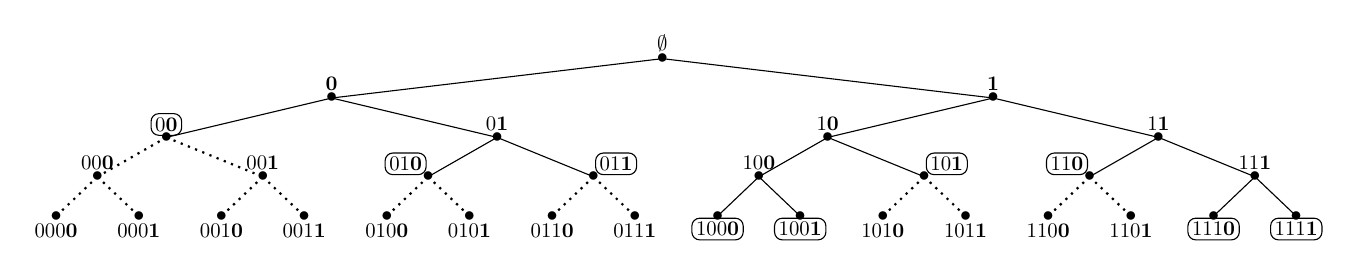
\begin{tikzpicture}[xscale=1.4]
\shorthandoff{>}
%
% nivel 2^4
%%%%%%%%%%%%
\draw[thick,dotted] (.375,.5)--(0,0) node[scale=.8]{$\bullet$} node[below,scale=.75]{000\textbf{0}};
\draw[thick,dotted] (.375,.5)--(.75,0) node[scale=.8]{$\bullet$} node[below,scale=.75]{000\textbf{1}};
\draw[thick,dotted] (1.875,.5)--(1.5,0) node[scale=.8]{$\bullet$} node[below,scale=.75]{001\textbf{0}};
\draw[thick,dotted] (1.875,.5)--(2.25,0) node[scale=.8]{$\bullet$} node[below,scale=.75]{001\textbf{1}};
\draw[thick,dotted] (3.375,.5)--(3,0) node[scale=.8]{$\bullet$} node[below,scale=.75]{010\textbf{0}};
\draw[thick,dotted] (3.375,.5)--(3.75,0) node[scale=.8]{$\bullet$} node[below,scale=.75]{010\textbf{1}};
\draw[thick,dotted] (4.875,.5)--(4.5,0) node[scale=.8]{$\bullet$} node[below,scale=.75]{011\textbf{0}};
\draw[thick,dotted] (4.875,.5)--(5.25,0) node[scale=.8]{$\bullet$} node[below,scale=.75]{011\textbf{1}};
%
\draw (6.375,.5)--(6,0) node[scale=.8]{$\bullet$}
node[inner sep=2pt,outer sep=1pt,draw=black,below,scale=.75,rounded corners=1mm]{100\textbf{0}};
%
\draw (6.375,.5)--(6.75,0) node[scale=.8]{$\bullet$}
node[inner sep=2pt,outer sep=1pt,draw=black,below,scale=.75,rounded corners=1mm]{100\textbf{1}};
%
\draw[thick,dotted] (7.875,.5)--(7.5,0) node[scale=.8]{$\bullet$} node[below,scale=.75]{101\textbf{0}};
\draw[thick,dotted] (7.875,.5)--(8.25,0) node[scale=.8]{$\bullet$} node[below,scale=.75]{101\textbf{1}};
\draw[thick,dotted] (9.375,.5)--(9,0) node[scale=.8]{$\bullet$} node[below,scale=.75]{110\textbf{0}};
\draw[thick,dotted] (9.375,.5)--(9.75,0) node[scale=.8]{$\bullet$} node[below,scale=.75]{110\textbf{1}};
%
\draw (10.875,.5)--(10.5,0) node[scale=.8]{$\bullet$}
node[inner sep=2pt,outer sep=1pt,draw=black,below,scale=.75,rounded corners=1mm]{111\textbf{0}};
%
\draw (10.875,.5)--(11.25,0) node[scale=.8]{$\bullet$}
node[inner sep=2pt,outer sep=1pt,draw=black,below,scale=.75,rounded corners=1mm]{111\textbf{1}};
%
%----------
%
% nivel 2^3
%%%%%%%%%%%%
\draw[thick,dotted] (1,1)--(.375,.5) node[scale=.8]{$\bullet$} node[above,scale=.75]{00\textbf{0}};
\draw[thick,dotted] (1,1)--(1.875,.5) node[scale=.8]{$\bullet$} node[above,scale=.75]{00\textbf{1}};
%
\draw (4,1)--(3.375,.5) node[scale=.8]{$\bullet$}
node[inner sep=2pt,outer sep=1pt,draw=black,above left,scale=.75,rounded corners=1mm]{01\textbf{0}};
%
\draw (4,1)--(4.875,.5) node[scale=.8]{$\bullet$}
node[inner sep=2pt,outer sep=1pt,draw=black,above right,scale=.75,rounded corners=1mm]{01\textbf{1}};
%
\draw (7,1)--(6.375,.5) node[scale=.8]{$\bullet$} node[above,scale=.75]{10\textbf{0}};
%
\draw (7,1)--(7.875,.5) node[scale=.8]{$\bullet$}
node[inner sep=2pt,outer sep=1pt,draw=black,above right,scale=.75,rounded corners=1mm]{10\textbf{1}};
%
\draw (10,1)--(9.375,.5) node[scale=.8]{$\bullet$}
node[inner sep=2pt,outer sep=1pt,draw=black,above left,scale=.75,rounded corners=1mm]{11\textbf{0}};
%
\draw (10,1)--(10.875,.5) node[scale=.8]{$\bullet$} node[above,scale=.75]{11\textbf{1}};
%
%----------
%
% nivel 2^2
%%%%%%%%%%%%
\draw (2.5,1.5)--(1,1) node[scale=.8]{$\bullet$}
node[inner sep=2pt,outer sep=1pt,draw=black,above,scale=.75,rounded corners=1mm]{0\textbf{0}};
%
\draw (2.5,1.5)--(4,1) node[scale=.8]{$\bullet$} node[above,scale=.75]{0\textbf{1}};
\draw (8.5,1.5)--(7,1) node[scale=.8]{$\bullet$} node[above,scale=.75]{1\textbf{0}};
\draw (8.5,1.5)--(10,1) node[scale=.8]{$\bullet$} node[above,scale=.75]{1\textbf{1}};
%
%----------
%
% nivel 2^1
%%%%%%%%%%%%
\draw (5.5,2)--(2.5,1.5) node[scale=.8]{$\bullet$} node[above,scale=.75]{\textbf{0}};
\draw (5.5,2)--(8.5,1.5) node[scale=.8]{$\bullet$} node[above,scale=.75]{\textbf{1}};
%
%----------
%
% nivel 2^0
%%%%%%%%%%%%
\draw (5.5,2) node[scale=.8]{$\bullet$} node[above,scale=.75]{$\emptyset$};

\end{tikzpicture} \end{center}
%
\leyenda{Arbol de  Kraft en el  caso binario ($d  = 2$). La ra\'iz,  de c\'odigo
  $\emptyset$ de largo 0, se divide en dos ramas, de c\'odigos respectivamente \
  $0$ \ y  \ $1$ \ (profundez \  $1$). Cada nudo de esta profundez  se divide en
  dos ramas (profundez dos), dando cuatros nuevos nudos con los c\'odigos \ $00$
  \ y $01$ de padre \ $0$, y \ $10$ \ y $11$ de padre \ $1$.  Etc.  En cada nudo
  de esta figura,  en el c\'odigo, se marca en  negrita la letra correspondiente
  al bit a\~nadido al c\'odigo padre.   Para hacer un c\'odigo libre de prefijo,
  una vez que un nudo es  seleccionado para ser una palabra c\'odigo (encuadrado
  en la  figura), no  puede tener nudos  ``hijos'' siendo tambi\'en  una palabra
  c\'odigo:  se boran  las ramas  saliendo  de un  nudo-palabra c\'odigo  (ramas
  punteadas).}
%
\label{Fig:SZ:ArbolKraft}
\end{figure}

El formalismo dado,  se va a ver ahora reaparecer la  entrop\'ia de Shannon como
cota de la codificaci\'on de fuente sin perdida:

\begin{teorema}[Cota inferior de c\'odigos descifrables]
\label{Teo:SZ:CotaInferiorCodigosDescifrables}
%
  Para  cualquier c\'odigo  \  $c$ \  descifrable  de la  fuente  $X$, su  largo
  promedio es  acotado por debajo  por la entrop\'ia  de Shannon de base  $d$ de
  $X$,
  %
  \[
  L(c) = \sum_{x \in \X} p_X(x) \, l_c(x) \: \ge \: H_d(X).
  \]
\end{teorema}
%
\begin{proof}
  \modif{Sea  \ $q_c(x)  = \frac{d^{-l_c(x)}}{\sum_{y  \in \X}  d^{-l_c(y)}}$, \
   distribuci\'on  de  probabilidad  por  construcci\'on. Del  lema~\ref  y  del
   lema~\ref{Lem:SZ:DescomposicionEntropiaCruzada} tenemos
  %
  \[
  L(c)   =   H_{\mathrm{cruz},d}\left(   \left.   q_c   \right\|   p_X   \right)
  - \log_d   \left(   \sum_{x   \in   \X}   d^{-l_c(x)}   \right)   =   H(X)   +
  D_{\mathrm{kl},d}\left(     \left.       p_X     \right\|      q_c     \right)
  - \log_d \left( \sum_{x \in \X} d^{-l_c(x)} \right)
  \]
  %Escribiendo \  $l_c(x) =
  %\log_d d^{-l_c(x)}$, \ se puede expresar el largo promedio de la forma
  %%
  %\[
  %L(c) =  - \sum_{x  \in \X}  p_X(x) \, \log_d  d^{-l_c(x)} =  - \sum_{x  \in \X}
  %p_X(x) \, \log_d q(x) - \log_d \sum_{x \in \X} d^{-l_c(x)}.
  %\]
  %
  %Notando que \ $- \log_d q  = \log_d \left( \frac{p_X}{q} \right) - \log_d p_X$
  %\ se obtiene
  %%
  %\[
  %L(c)  = H_d(X)  + D_{\mathrm{kl},d}\left(  \left.   p_X \right\|  q \right)  -
  %\log_d \sum_{x \in \X} d^{-l_c(x)}.
  %\]
  %%
  }
  El resultado proviene de la  positividad de la divergencia de Kullback-Leibler
  y de la desigualdad de Kraft-McMillan (el argumento del logaritmo siende menor
  que $1$).
\end{proof}
%
\noindent Este  resultado significa que la  taza de compresi\'on  sin perdida no
puede  ser m\'as  bajo que  el  contenido informacional  de la  fuente. En  este
sentido, $H$ tiene realmente un sabor de informaci\'on sobre la fuente $X$.

La entrop\'ia aparece tambi\'en en la cota superior del c\'odigo \'optimo:
%
\begin{teorema}[Cota superior del c\'odigo descifrable \'optimo]
\label{Teo:SZ:CotaSuperiorCodigoDescifrableOptimo}
%
  El largo promedio \ $L^\opt$ \ del c\'odigo \ $c^\opt$ \ descifrable, de largo
  promedio m\'inimo es  acotado por arriba por la entrop\'ia  de Shannon de base
  $d$ de $X$ m\'as un {\it dit} (1 s\'imbolo de $\C$),
  %
  \[
  L^\opt \: < \: H_d(X) + 1.
  \]
\end{teorema}
%
\begin{proof}
  Por  eso,  empezamos  por  buscar  los  largos  \'optimos,  soluci\'on  de  la
  optimizaci\'on
  %
  \[
  \min \sum_{x \in \X} p_X(x) \,  l(x) \qquad \mbox{sujeto a} \qquad \sum_{x \in
    \X} d^{-l(x)} \, \le \, 1.
  \]
  %
  %Sea \ $q(x)  = \frac{d^{-l_c(x)}}{\sum_{x \in \X} d^{-l_c(x)}}$,  \ siendo una
  %distribuci\'on de  probabilidad por  construcci\'on.  
  Escribiendo  \ $l_c(x) =  \log_d d^{-l_c(x)}$,  \ se  puede expresar  el largo
  promedio de la forma
  %
  \[
  L(c) =  - \sum_{x  \in \X}  p_X(x) \, \log_d  d^{-l_c(x)} =  - \sum_{x  \in \X}
  p_X(x) \, \log_d q(x) - \log_d \sum_{x \in \X} d^{-l_c(x)}.
  \]
  %
  Olvidando que los  \ $l_i \equiv l_c(x_i)$ \ son enteros,  $L(c)$ es convexa con
  respecto  a los $l_i$  as\'i que  el v\'inculo,  garantizando que  el m\'inimo
  existe y es \'unico.  El problema se resuelva con el enfoque KKT (Ver
    nota de pie~\ref{Foot:SZ:KKT}),
  % pagina~\pageref{Foot:SZ:KKT}.}, 
    optimizaci\'on  con  v\'inculos  tipo desigualdades~\cite{Mil00,  CamMar09},
    conduciendo a los ``largos''
  %
  \[
  \widetilde{l}(x) = - \log_d p_X(x).
  \]
  %
  $\widetilde{l}(x)$ no es necesariamente entero, as\'i que una posibilidad para
  volver  a largos  enteros  puede ser  de  tomar la  parte  entera superior  de
  $\widetilde{l}(x)$,
  %
  \[
  l(x) = \Big\lceil\! - \log_d p_X(x) \Big\rceil.
  \]
  %
  Obviamente el  conjunto de largos satisface la  desigualdad de Kraft-McMillan,
  as\'i que  se puede construir un  c\'odigo \ $c^\sh$ \  descrifrable con estos
  largos. De \ $l(x) < - \log_d p_X(x) + 1$ se obtiene
  %
  \[
   L^\opt \le L\left( c^\sh \right) < H_d(X) + 1.
  \]
  %
\end{proof}
%
De \[  H_d(X) \le  L^\opt < H_d(X)  + 1 \]  se revela  el rol fundamental  de la
entrop\'ia en la  codificaci\'on de fuente sin perdida.   La codificaci\'on es a
veces  dicha {\it  codificaci\'on  entr\'opica} y  da  un rol  operacional a  la
entrop\'ia  de  Shannon.   Se   notar\'a  tambi\'en  que  de  la  demostraci\'on
precediente  de   que  aparece  un   c\'odigo  particular  a  trav\'es   de  los
$\Big\lceil\!  - \log_d p_X(x) \Big\rceil$:
%
\begin{definicion}[C\'odigo de Shannon]
\label{Def:SZ:ShannonCode}
%
  Un  c\'odigo  \  $c^\sh$  \  de  una  fuente $X$,  de  largos  \  $l^\sh(x)  =
  \Big\lceil\!   - \log_d  p_X(x) \Big\rceil$,  \ libre  de  prefijo (construido
  sobre el arbol de Kraft) es llamado {\it c\'odigo de Shannon}.
\end{definicion}
%
Obviamente, tambi\'en
%
\[
H_d(X) \le L\left( c^\sh  \right) < H_d(X) +  1.
\]
%
Al lo contrario de primer vista, un  c\'odigo de Shannon no es \'optimo, como se
lo puede ver con el ejemplo siguiente.
%
\begin{ejemplo}
\label{Ej:SZ:CodigoShannonNoOpt}
%
  Sea \ $\X  = \C = \{ 0 \,  , \, 1 \}$ \  y una fuente $X$ tal que  \ $p_X(0) =
  0.999 = 1 - p_X(1)$.   Los largos de Shannon van a ser \ $l^\sh(0)  = 1$ \ y \
  $l^\sh(1) = 10$,  y el largo promedio vale \ $L\left(  c^\sh \right) = 1.009$.
  Obviamente, un c\'odigo \'optimo es \ $c(x) =  x$ \ de largos \ $l_c(x) = 1$ \
  dando \ $L^\opt = 1$ bit.
\end{ejemplo}
%
De hecho, volviendo al problema  con largos virtualmente no enteros, el m\'inimo
se alcanza para  $\widetilde{l}(x) = - \log_d p_X(x)$, es  decir que, los largos
siendo enteros, se alcanza la cota m\'inima del c\'odigo \'optimo si y solamente
si $- \log_d p_X(x)$.  Una distribuci\'on satifaciendo esta condici\'on es dicha
$d$-\'adica.   Sin embargo,  el c\'odigo  de  Shannon es  ``competitivo'' en  el
sentido de que:
%
\begin{teorema}[Competitividad del c\'odigo de Shannon]
\label{Teo:SZ:CompetitividadCodigoShannon}
%
Sea  $X$ \ fuente  sobre \  $\X$, de  distribuci\'on \  $p_X$ \  y \  $c^\sh$ el
c\'odigo de Shannon asociado  sobre el alfabeto c\'odigo \ $\C =  \{ \cod_1 \, ,
\,  \ldots \, ,  \, \cod_d  \}$, de  largos $l^\sh(x)  = \Big\lceil\!   - \log_d
p_X(x) \Big\rceil$.  Para cualquier c\'odigo  \ $c$ \ descifrable y cualquier $k
\ge 1$,
  %
  \[
  P\Big( l^\sh(X) \ge l_c(X) + k \Big) \le \frac{1}{d^{k-1}}.
  \]
\end{teorema}
%
\begin{proof}
  Por definici\'on de la parte entera superior, $a + 1 > \lceil a \rceil$, as\'i
  que $\lceil a \rceil \ge b \: \Rightarrow \: a > b-1$. A continuaci\'on, de la
  implicaci\'on de eventos $(Y  \ge a) \varsubsetneq (Y \ge b-1)$ \  dando $P(A \ge a)
  \le P(Y \ge b-1)$ \ y de la definici\'on de un c\'odigo de Shannon se obtiene
  %
  \begin{eqnarray*}
  P\Big( l^\sh(X)  \ge l_c(X) + k  \Big) & \le & P\Big(  - \log_d p_X(X)
  \ge  l_c(X) + k  - 1  \Big)\\[2.5mm]
  %
  & = &  P\Big( p_X(X)  \le d^{-l_c(X)  - k  + 1} \Big)\\[2.5mm]
  %
  & = &  \sum_{x \in \X : p_X(x) \le d^{-l_c(x)  - k  + 1}} p_X(x)
  \end{eqnarray*}
  %
  Pero, sumando sobre  lo $x$ tal que $p_X(x) \le d^{-l_c(x)  - k + 1}$,
  se obtiene
  %
  \[
  P\Big( l^\sh(X)  \ge l_c(X) + k  \Big) \le \frac{1}{d^{k-1}} \sum_{x  \in \X :
    p_X(x) \le d^{-l_c(x) - k + 1}} d^{-l_c(x)}
  \le \frac{1}{d^{k-1}} \sum_{x \in \X} d^{-l_c(x)}
  \]
  %
  (a\~nadiendo t\'erminos positivos en la suma). La prueba se cierra notando que
  $c$ siendo descifrable, $l_c$ satisface la desigualdad de Kraft-McMillan.
\end{proof}
%
Este  teorema traduce  el hecho  que a  pesar de  que $c^\sh$  no  sea \'optimo,
tomando  cualquier otro c\'odigo,  incluyendo el  \'optimo, la  probabilidad que
$c^\sh(X)$ tenga un largo m\'as grande que $c(X)+k$ decrece exponencialmente con
$k$.
%
\begin{ejemplo}
\label{Ej:SZ:CompetitividadCodigoShannon}
%
  De manera general, con $d = 2$ y para $k = 9$, $P\Big( l^\sh(X) \ge l_c(X) + 9
  \Big)      \le       0.391      \%$.      En       particular,      en      el
  ejemplo~\ref{Ej:SZ:CodigoShannonNoOpt},    notando    que    s\'olo   en    la
  codificaci\'on de $x=1$ se puede tener $l^\sh(x) \ge l_c(x) + 9$, si no se usa
  1 bit, este resultado significa que la probabilidad de usar m\'as de 1 bit con
  el c\'odigo de Shannon es menor que $0.391 \%$. De hecho, una palabra c\'odigo
  de largo $10$ aparece con una probabilidad $0.1\%$\ldots
\end{ejemplo}

En el problema  de minimizaci\'on, el hecho que los largos  deben ser enteros no
permite solucionar explicitamente el problema de busqueda del c\'odigo \'optimo.
N\'umeros investigadores  contruyeron c\'odigos,  intentando probar de  que eran
\'optimos (ver  ej.~\cite{Sha48, ShaWea64,  Fan49} por los  primeros, y~\cite[\&
ref.]{CovTho06}).  El c\'odigo conocido  como {\it c\'odigo de Fano}~\footnote{A
  pesar  de que  sea  diferente del  de Shannon  y  que cada  uno fueron  hechos
  independientemente, a veces  es conocido como c\'odigo de  Fano-Shannon, o aun
  Shannon-Fano-Elias~\cite{CovTho06, KraLiu15}.}  \ $c^\fa$  \ se basa  sobre el
hecho de que se alcanza la cota m\'inima para una distribuci\'on $d$-\'adica.
%
\begin{definicion}[C\'odigo de Fano]
\label{Def:SZ:FanoCode}
%
  El  principio  es  de  clasificar   los  estados  de  $\X$  para  obtener  las
  probabilidades clasificadas en  orden decreciences ($p_X^\downarrow$).  Luego,
  se divide $\X$ en $d$ ensembles a  lo m\'as equiprobables que se puede (\ie de
  probabilidad a lo  m\'as cerca de $d^{-1}$) y de  asignar $\cod_i$ al conjunto
  $i$.   Luego,   se  repite  el   proceso  a  cada  sub-conjunto   (para  tener
  sub-conjuntos de probabilidades a lo m\'as cerca de $d^{-2}$) y al subconjunto
  $j$ del conjunto $i$ se va a asignar le c\'odigo $\cod_i \cod_j$, etc.  Eso es
  ilustrado en la figura Fig.~\ref{Fig:SZ:FanoHuffmanCodes}-(a).
\end{definicion}
%
\SZ{Probar/mencionar  que  tambi\'en  \[   H(X)  \le  L\left(  c^\fa  \right)  <
  H(X)+1. \]}
%  \qquad \mbox{con}  \qquad L^\fa  =  L_{c^\fa}$$}

Fijense de que no hay un \'unico c\'odigo  de Fano o de Shannon (tal como no hay
un \'optimo  \'unico).  Por exemple, hacer  una permutacion de  los $\cod_i$ da
los mismos  largos y  el mismo largo  promedio sin  cambiar el aspecto  libre de
prefijo. De la  misma manera, en el  arbol de Kraft, en cada  profundez se puede
permutar los s\'imbolos  asociados a las hojas de esta  profundez sin cambiar el
aspecto libre de  prefijo y sin que cambien los largos  $l(x_i)$ (y entonces con
el mismo largo promedio).

Una soluci\'on para construir un  c\'odigo \'optima fue propuesta por Huffman en
1951-1952~\cite{Huf52,  Pig03}~\footnote{De hecho,  Huffman  fue estudiantes  de
  maestria  de Fano,  trabajando  en el  MIT.  Su  tesis  era de  probar que  el
  c\'odigo de Fano  era \'optimo: Huffman propus\'o su  propio c\'odigo, andando
  al rev\'es del enfoque de Fano, y demostr\'o que era \'optimo~\cite{Sti91}.}
%
\begin{definicion}[C\'odigo de Huffman]
\label{Def:SZ:HuffmanCode}
%
  Suponemos que  existe un $\beta \in  \Nset$ tal que~\footnote{Si  no, se puede
    elegir $\beta =  \left\lceil \frac{\alpha-d}{d-1} \right\rceil$, y completar
    $\X$  con  $d  +  \beta  (d-1)  -  \alpha$  s\'imbolos  fuente  fictivos  de
    probabilidades ceros, lo  que no va a cambiar ni la  entrop\'ia, ni el largo
    promedio del  c\'odico aferente.}   $\alpha =  |\X| = d  + \beta  (d-1)$. El
  algoritmo de Huffman consiste a construir un arbol donde cada nudo es asociado
  a un conjunto de s\'imbolos fuente y una letra de $\C$ de la manera siguiente:
  %
  \begin{enumerate}
  \item\label{Huffman:clasificar}   Clasificar  las   probabilidades   en  orden
    decrecientes: por cambio de escritura, llamamos \ $p_i$ \ las probabilidades
    rearregladas, y \ $x_i$ \ los s\'imbolo fuente correspondientes.
  %
  \item\label{Huffman:codigolocal}  A  cada \  $x_i,  \:  \alpha-d+1  \le i  \le
    \alpha$ ($d$  probabilidades m\'as debiles), \  associar un nudo  y la letra
    ``hijo'' \ $\cod_i$.
  %
  \item\label{Huffman:padre} Crear \ $d$ \ ramas saliendo de un nudo padre hasta
    los $d$ nudos $x_i, \: \alpha-d+1 \le i \le \alpha$.
  %
  \item\label{Huffman:reconfiguracion}  Crear un  nuevo  conjunto de  s\'imbolos
    fuente  \  $\widetilde{x}_i   =  x_i,  \:  1  \le  i   \le  \alpha-d$  \  de
    probabilidades   respectivas    \   $\widetilde{p}_i   =   p_i$    \   y   \
    $\widetilde{x}_{\alpha-d+1} = \{  x_j, \: \alpha-d+1 \le j  \le \alpha \}$ \
    de probabilidad  \ $\widetilde{p}_{\alpha-d+1}  = p_{\alpha-d+1} +  \ldots +
    p_\alpha$.  El \'ultimo ``super-s\'imbolo'' fuente es asociado al nudo padre
    de la etapa~\ref{Huffman:padre}.
  %
  \item  Si   quedan  m\'as  de   un  (super-)s\'imbolo  fuente,  volver   a  la
    etapa~\ref{Huffman:clasificar}  con \  $p  \equiv \widetilde{p}$  \  y \  $x
    \equiv \widetilde{x}$.
  \end{enumerate}
  %
  Como descrito tratando del c\'odigo usando  el arbol de Kraft, se construye el
  arbol saliendo de las hojas, y  luego, el c\'odigo \ $c^\huf(x_i)$ \ se deduce
  saliendo de  la ra\'iz  del arbol as\'i  construido, agregando las  letras del
  camino que  llega hasta  la hoja  \ $x_i$.  \  Eso es  ilustrado en  la figura
  Fig.~\ref{Fig:SZ:FanoHuffmanCodes}-(b) en el caso binario.
\end{definicion}
%
Se mencionar\'a que  a cada etapa, el nuevo  conjunto de super-s\'imbolos fuente
contiene   exactamente   \  $d-1$   \   s\'imbolos   menos   que  a   la   etapa
precediente.  As\'i, con  \ $\alpha  = d  + \beta  (d-1)$ \  el  algoritmo tiene
exactamente \ $\beta+1$ \ bucles y  en cada profundez no hay ning\'un nudo vacio
en  el sentido  que  o  es una  hoja,  o es  un  nudo padre/prefijo  (quedar\'an
exactamente $d$ nudos a agregar a la ra\'iz en la \'ultima etapa).  Por exemplo,
con \ $d = 3$ \ si tuvieramos \ $\alpha = 4$, en la segunda etapa tendriamos $2$
estados  a juntar,  dando un  c\'odigo de  largos $2,  2, 2,  1$.   Empezando la
primera etapa  con la asociaciaci\'on de  $2$ estados, es decir  $3$ teniendo en
cuenta un estado fictivo  ($\alpha = 5$, $\beta = 1$) van  a quedar 3 estados en
la segunda etapa,  dando un c\'odigo de largos  $2, 2, 1, 1$, es  decir de largo
promedio m\'as peque\~no.

\begin{teorema}[\'Optimalidad del c\'odigo de Huffman]
\label{Teo:SZ:OptimalidadHuffman}
%
  El algoritmo de Huffman da un c\'odigo \ $c^\huf$ \ de largo promedio m\'inimo
  en  la  clase de  los  c\'odigos  descrifrables y  los  libre  de prefijo  (se
  recordar\'a que  con los  largos de c\'odigos  descifrables, siempre  se puede
  construir un c\'odigo  libre de prefijo), es decir \  $L^\opt = L\left( c^\huf
  \right)$.
\end{teorema}
%
\begin{proof}
  Una  prueba  es  dada  por  ejemplo en~\cite[Sec.~5.8]{CovTho06}  en  el  caso
  binario, pero la  extensi\'on para $d >  2$ es un poco m\'as  sutil. La prueba
  m\'as general  es dada  por Huffman~\cite{Huf52} y  se consigue  tambi\'en por
  parte en~\cite{Pig03}.   Suponemos que  $\beta \ge 1$  (sino, el  resultado es
  obvio). Las etapas son
  %
  \begin{itemize}
  \item Sean $j,  k$ dos indices. Si \  $c^\opt$ \ es un c\'odigo  \'optimo, y \
    $c$ \ un c\'odigo tal que \ $l(x_i) = l^\opt_i, \quad i \ne j , k, \quad l_j
    = l^\opt_k  \quad \& \quad  l_k = l^\opt_j$,  \ se obtiene  \ $0 \le  L(c) -
    L^\opt  = \sum_i p_i  \left( l_i  - l^\opt_i  \right) =  (p_j -  p_k) \left(
      l^\opt_k  - l^\opt_j  \right)$.   \  Entonces $p_j  >  p_k \:  \Rightarrow
    l^\opt_j \le l^\opt_k$.
  %
  \item Sea  $\eta$ el n\'umero  de s\'imbolos fuente  con un c\'odigo  de largo
    m\'aximo \ $l_{\max}$ \ y \ $\eta' = \min(\eta,d)$.  Del punto anterior, los
    $\eta$  s\'imbolos  con  palabra  c\'odigo  de largo  m\'aximo  son  los  de
    probabilidades m\'as peque\~nas.
  %
  \item  Como descrito  antes, se  puede permutar  las letras  c\'odigos  de una
    profundez del arbol de Kraft sin  cambiar ni el aspecto libre de prefijo, ni
    el largo promedio. Se puede entonces considerar el c\'odigo \'optimo tal que
    los  $\eta'$ s\'imbolos  de probabilidades  las m\'as  peque\~nas  tienen el
    mismo  nudo padre,  \ie solamente  la \'ultima  letra c\'odigo  cambia entre
    ellos.
  %
  \item  Suponemos que  \ $\eta'  = \eta  < d$.   \ Sea  una  ``super-fuente'' \
    $\X^{(2)}  =  \left\{  x^{(2)}_i  \right\}_{i=1}^{\alpha-\eta'+1}$ \  con  \
    $x^{(2)}_i  = x_i,  \quad  1 \le  i  \le \alpha-\eta'$  \ de  probabilidades
    respectivas  \  $p(x_i)$  \  y  \ $x^{(2)}_{\alpha-\eta'+1}  \equiv  \{  x_i
    \}_{i=\alpha-\eta'+1}^\alpha$  \  de  probabilidad \  $p_{\alpha-\eta'+1}  +
    \cdots   +  p_\alpha$   \   (se   ``plegan''  las   $\eta'$   hojas  en   un
    super-s\'imbolo).    La   c\'odificaci\'on    \'optima   es   entonces   una
    codificaci\'on libre de prefijo de $\X^{(2)}$, ``arbol ra\'iz'' del c\'odigo
    \'optimo, a la cual se a\~nade  una letra c\'odigo $\cod_j$ diferente a cada
    s\'imbolo  del  super-s\'imbolo  $x^{(2)}_{\alpha-\eta'+1}$.   La  profundez
    m\'axima del  c\'odigo arbol  es \ $l_{\max}-1$  \ y  debe ser llena,  en el
    sentido de que no debe tener un nudo que sea ni una hoja, ni un prefijo.  En
    el    caso   contrario,    se   podr\'ia    desplazar   un    s\'imbolo   de
    $x^{(2)}_{\alpha-\eta'+1}$ al  nudo ``vacio'' de  la profundez $l_{\max}-1$,
    sin cambiar  el aspecto  libre de prefijo,  pero ganando una  letra c\'odigo
    sobre un  s\'imbolo, \ie  hacer un  c\'odigo libre de  prefijo con  un largo
    promedio  menor.  Ser\'ia  contradictorio  con la  optimalidad del  c\'odigo
    inicial.
  % 
  \item  Para   c\'odificar  $\X^{(2)}$,  se  necesita  por   lo  menos  $\lceil
    \log_d(\alpha-\eta'+1)  \rceil$  profundez  en  el arbol  ra\'iz.   En  esta
    profundez   (m\'axima   en   el    caso   optimista),   hay   \   $d^{\lceil
      \log_d(\alpha-\eta'+1) \rceil} \ge \alpha-\eta'+1$ \ nudos. En la \'ultima
    profundez  pueden  ser  todos  ocupados  si  y  solamente  si  \  $d^{\lceil
      \log_d(\alpha-\eta'+1) \rceil}  = \alpha-\eta'+1$.  En  otras palabras, es
    posible si  y solamente si  existe un entero  $k$ tal que  $\alpha-\eta'+1 =
    d^k$, es decir, con \ $\alpha = d + \beta (d-1)$, \ que teniamos el entero \
    $\beta = \frac{d^k-d}{d-1} +  \frac{\eta'-1}{d-1}$.  \ La primera fracci\'on
    \ $\frac{d^k-d}{d-1}  = d^{k-1} +  \cdots + 1$  \ siendo entera,  $\beta$ no
    puede ser entero  con \ $\eta' < d$.  \  En otros t\'erminos, necesariamente
    $\eta' = d$, \ie los $d$  s\'imbolos de probabilidad m\'as debiles son el la
    \'ultima profundez y se puede elegir que comparten el mismo nudo padre.
  %
  \item Sea \ $c^{\opt,(1)}$ \ el c\'odigo \'optimo correspondiente a \ $\X$ \ y
    \ $c^{(2)}$  \ el  c\'odigo ``padre'' sobre  \ $\X^{(2)}$  \ ($c^{\opt,(1)}$
    quitando la \'ultimo  letra c\'odigo de los s\'imbolos  juntados, \ie con la
    ra\'iz  com\'un de  estos).  De  la misma  manera, sea  \  $c^{\opt,(2)}$ un
    c\'odigo  \'optimo sobre  $\X^{(2)}$ \  y \  $c^{(1)}$ \  el que  se obtiene
    deplegando el super-s\'imbolo \ $x^{(2)}_{\alpha-d+1}$ \ en $d$ hojas.  De \
    $L^{\opt,(1)}  =  L\left(  c^{(2)}  \right)  +  p_{\alpha-d+1}  +  \cdots  +
    p_\alpha$ \ (pasar de $\X^{(2)}$ a  $\X$ se a\~nade solo una letra palabra a
    los  s\'imbolos  del super-s\'imbolo)  \  y  \  $L\left( c^{(1)}  \right)  =
    L^{\opt,(2)}  + p_{\alpha-d+1} +  \cdots +  p_\alpha$ \  se obiene  \ $\Big(
    L^{\opt,(1)} - L\left( c^{(1)} \right)  \Big) + \Big( L^{\opt,(2)} - L\left(
      c^{(2)}  \right) \Big)  \: =  \: 0$.   \ Cada  t\'ermino  entre parentesis
    siendo positivo, valen necesariamente  cero (la suma de t\'erminos positivos
    vale cero si y solamente si  todos son nulos).  En conclusi\'on, \ $c^{(2)}$
    \  padre   de  \  $c^{\opt,(1)}$   \  queda  \'optimo,  \   $c^{(2)}  \equiv
    c^{\opt,(2)}$ \ (y \ $c^{(1)} \equiv c^{\opt,(1)}$).
  %
  \item Notando que \ $|\X^{(2)}| = \alpha - (\beta-1) (d-1)$, \ el razonamiento
    se   propaga  por   inducci\'on,  pasando   de  \   $c^{\opt,(k)}$  \   a  \
    $c^{\opt,(k+1)}$ \ juntando los $d$ super-s\'imbolos de probabilidades m\'as
    debiles,  hasta tener  un  super-s\'imbolo tendiendo  todos los  s\'imbolos,
    $\left| \X^{(K)} \right| = 1$, ra\'iz del arbol.
\end{itemize}
\end{proof}
%
De esta  prueba, se puede ver que
%
\begin{itemize}
\item  Cada  profundez siendo  llena,  los largos  obtenidos  van  a saturar  la
  desigualdad de Kraft-McMillan.
%
\item Si \ $\frac{\alpha  - d}{d-1}$ \ no es entero, en  lugar de completar $\X$
  con s\'imbolos fictivos se puede  empezar el algoritmo de Huffman juntando los
  \ $\alpha - d - \left\lfloor \frac{\alpha - d}{d-1} \right\rfloor (d-1) + 1$ \
  s\'imbolos fuentes  de probabilidades m\'as  debiles en un  super-s\'imbolo, y
  luego hacer el bucle descrito (juntando por super-s\'imbolos de $d$ s\'imbolos
  en  cada  bucle);  en  este  caso,  no  se  satura  m\'as  la  desigualdad  de
  Kraft-McMillan, pero  no es contradictorio  con el punto anterior  que contaba
  los largos de estados fictivos (que no codificamos en realidad).
%
\item Obviamente, en el caso binario $d = 2$, no es necesario completar $\X$ por
  estados fuentes, o  empezar con menos de $d$  s\'imbolos juntados ($\alpha$ es
  necesariamente de la forma $\alpha = d + \beta (d-1) = 2 + \beta$).
%
\item  El algoritmo  no  permite conocer  los  largos de  manera anal\'itica  en
  funci\'on  de $p_i$,  y  tampoco el  largo  promedio.  Se  los pueden  deducir
  solamente  implementando   el  algoritmo  (una   vez  que  es   construido  el
  c\'odigo). Era el caso tambi\'en con el enfoque de Fano.
\end{itemize}

Volviendo al c\'odigo  ingenuo, ser\'ia \'optimo (y equivalente a  los de Fano y
de Shannon) para una distribuci\'on uniforme. En este contexto, la entrop\'ia es
$H_d(X) = \log_d |\X|$, precisamente la incerteza del enfoque de Hartley
que   corresponde  a   los   n\'umeros  de   dits   necesarios  para   codificar
(ingenuosamente) la fuente.

\begin{figure}[h!]
\begin{center} 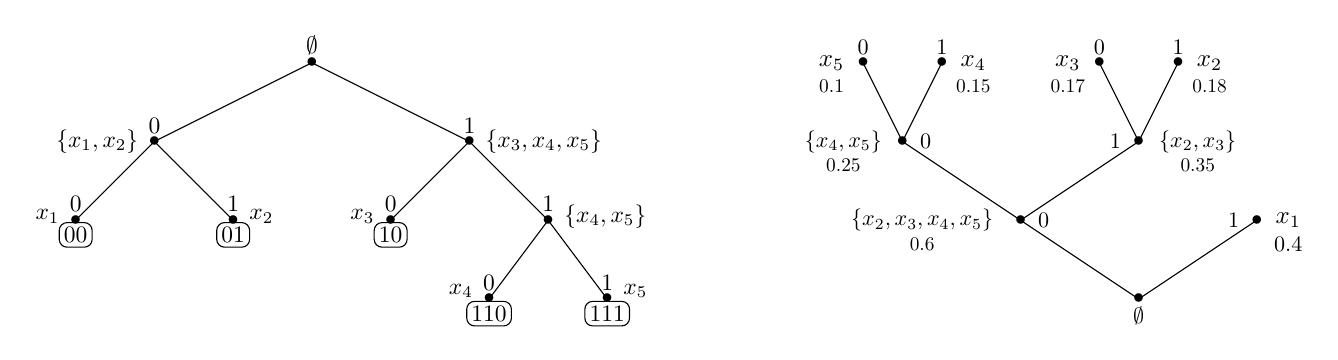
\begin{tikzpicture}%[xscale=3.5,yscale=3]
\shorthandoff{>}
%
% Codigo de Fano
\begin{scope}
\draw(0,0) node[scale=.8]{$\bullet$} node[above,scale=.85]{$\emptyset$};
%
% -----
%
\draw (0,0) -- (-2,-1) node[scale=.8]{$\bullet$} node[above,scale=.85]{$0$};
\draw (-2.1,-1) node[left,scale=.85]{$\{ x_1,x_2\}$};
%
\draw (0,0) -- (2,-1) node[scale=.8]{$\bullet$} node[above,scale=.85]{$1$};
\draw(2.1,-1) node[right,scale=.85]{$\{ x_3,x_4,x_5\}$};
%
% -----
%
\draw (-2,-1) -- (-3,-2) node[scale=.8]{$\bullet$} node[above,scale=.85]{$0$}
node[inner sep=2pt,outer sep=1pt,draw=black,below,scale=.85,rounded corners=1mm]{$00$};
\draw (-3.1,-1.95) node[left,scale=.85]{$\boldsymbol{x_1}$};
%
\draw (-2,-1) -- (-1,-2) node[scale=.8]{$\bullet$} node[above,scale=.85]{$1$}
node[inner sep=2pt,outer sep=1pt,draw=black,below,scale=.85,rounded corners=1mm]{$01$};
\draw (-.9,-1.95) node[right,scale=.85]{$\boldsymbol{x_2}$};
%
\draw (2,-1)-- (1,-2) node[scale=.8]{$\bullet$} node[above,scale=.85]{$0$}
node[inner sep=2pt,outer sep=1pt,draw=black,below,scale=.85,rounded corners=1mm]{$10$};
\draw (.9,-1.95) node[left,scale=.85]{$\boldsymbol{x_3}$};
%
\draw (2,-1)-- (3,-2) node[scale=.8]{$\bullet$} node[above,scale=.85]{$1$};
\draw (3.1,-1.95) node[right,scale=.85]{$\{ x_4 , x_5 \}$};
%
% -----
%
\draw (3,-2)-- (2.25,-3) node[scale=.8]{$\bullet$} node[above,scale=.85]{$0$}
node[inner sep=2pt,outer sep=1pt,draw=black,below,scale=.85,rounded corners=1mm]{$110$};
\draw (2.15,-2.9) node[left,scale=.85]{$\boldsymbol{x_4}$};
%
\draw (3,-2)-- (3.75,-3) node[scale=.8]{$\bullet$} node[above,scale=.85]{$1$}
node[inner sep=2pt,outer sep=1pt,draw=black,below,scale=.85,rounded corners=1mm]{$111$};
\draw (3.85,-2.9) node[right,scale=.85]{$\boldsymbol{x_5}$};
\end{scope}
%
%
% Codigo de Huffman
\begin{scope}[xshift=12cm]
\draw (-5,0) node[scale=.8]{$\bullet$} node[above,scale=.8]{$0$}
-- (-4.5,-1) node[scale=.8]{$\bullet$} node[right,scale=.8]{$\:\: 0$}
-- (-4,0) node[scale=.8]{$\bullet$} node[above,scale=.8]{$1$};
\draw(-5.4,0) node[scale=.9]{$\boldsymbol{x_5}$};
\draw(-5.4,-.3) node[scale=.7]{$0.1$};
\draw(-3.6,0) node[scale=.9]{$\boldsymbol{x_4}$};
\draw(-3.6,-.3) node[scale=.7]{$0.15$};
\draw(-5.25,-1) node[scale=.8]{$\{x_4,x_5\}$};
\draw(-5.25,-1.3) node[scale=.7]{$0.25$};
%
% -----
%
\draw (-2,0) node[scale=.8]{$\bullet$} node[above,scale=.8]{$0$}
-- (-1.5,-1) node[scale=.8]{$\bullet$} node[left,scale=.8]{$1\:\: $}
-- (-1,0) node[scale=.8]{$\bullet$} node[above,scale=.8]{$1$};
\draw(-2.4,0) node[scale=.9]{$\boldsymbol{x_3}$};
\draw(-2.4,-.3) node[scale=.7]{$0.17$};
\draw(-.6,0) node[scale=.9]{$\boldsymbol{x_2}$};
\draw(-.6,-.3) node[scale=.7]{$0.18$};
\draw(-.75,-1) node[scale=.8]{$\{x_2,x_3\}$};
\draw(-.75,-1.3) node[scale=.7]{$0.35$};
%
% -----
%
\draw (-4.5,-1) -- (-3,-2) node[scale=.8]{$\bullet$} node[right,scale=.8]{$\:\: 0$} -- (-1.5,-1);
\draw(-4.25,-2) node[scale=.8]{$\{x_2,x_3,x_4,x_5\}$};
\draw(-4.25,-2.3) node[scale=.7]{$0.6$};
%
% -----
%
\draw (-3,-2) -- (-1.5,-3) node[scale=.8]{$\bullet$} node[below,scale=.8]{$\emptyset$}
-- (0,-2) node[scale=.8]{$\bullet$} node[left,scale=.8]{$1\:\:$};
\draw(.4,-2) node[scale=.9]{$\boldsymbol{x_1}$};
\draw(.4,-2.3) node[scale=.8]{$0.4$};
\end{scope}
\end{tikzpicture} \end{center}
%
\leyenda{Construcci\'on de  un c\'odigo binario  sobre $\C =  \{0 \, , \,  1 \}$
  asociado al vector de probabilidad $p_X = \protect\begin{bmatrix} 0.4 & 0.18 &
    0.17 & 0.15 & 0.1 \protect\end{bmatrix}^t$ sobre el arbol de Kraft.  En este
  caso, $H_2(X)  \approx 2.1514$\ (a): Enfoque  de Fano, saliendo  de la ra\'iz.
  En cada nudo, se menciona el conjunto de s\'imbolos que va a tener el c\'odigo
  correspondiente  (en negro  cuando  es un  solo  s\'imbolo).  Se  pasa de  una
  profundez  a la  otra  dividiendo los  conjunto  en sub-conjuntos  a lo  m\'as
  equiprobables.   Esta construcci\'on  da el  c\'odigo \  $c^\fa(x_1) =  00, \:
  c^\fa(x_2) = 01, \: c^\fa(x_3) = 10, \: c^\fa(x_4) = 110, \: c^\fa(x_5) = 111$
  \ de  largo promedio \ $L\left(  c^\fa \right) =  2.25$.  \ \ (b):  Enfoque de
  Huffman, saliendo de las hojas.   En cada nudo, se menciona el correspondiente
  (i) conjunto de s\'imbolos,  (ii) $\cod_i$ de esta profundez/posici\'on, (iii)
  la probabilidad  asociada al  conjunto.  Se  pasa de una  profundez a  la otra
  juntando  los conjuntos  menos  probables en  sobre-conjuntos.   En negro  son
  indicados los s\'imbolos simples: van a tener el c\'odigo agregando los de los
  nudos yendo de la ra\'iz hasta  las hojas.  Esta construcci\'on da el c\'odigo
  \ $c^\huf(x_1) = 1, \: c^\huf(x_2) = 011, \: c^\huf(x_3) = 010, \: c^\huf(x_4)
  = 001, \: c^\huf(x_5) = 000$ \ de largo promedio \ $L^\opt = 2.2$.}
%
\label{Fig:SZ:FanoHuffmanCodes}
\end{figure}


Se notar\'a  de que, tratando  de una fuente  \ $\{ X_t  \}_{t \in \Zset}$  \ de
variables independientes,  se puede  codificar la fuente  con un  largo promedio
arbitrariamente cerca  de $H_d(X)$.   El principio es  de considerar  vectores \
$\begin{bmatrix} X_1 & \cdots &  X_n \end{bmatrix}^t$ \ viviendo sobre \ $\X^n$,
llamado {\it extensi\'on de orden $n$ de la fuente}, con un c\'odigo descifrable
(o libre de  prefijo) de esta extensi\'on; es llamado  {\it codificaci\'on de la
  extensi\'on  de  la  fuente}  pero  no  es  necesariamente  una  extension  de
$c$. As\'i, \ $H_d(X_1 , \ldots ,  X_n) \le L^{\opt,n} < H_d(X_1 , \ldots , X_n)
+ 1$, es decir, de la independencia,
%
\[
H_d(X)  \:  \le \:  \frac{L^{\opt,n}}{n}  \: <  \:  H_d(X)  + \frac{1}{n}  \quad
\mbox{por s\'imbolo}
\]
%
(ver  tambi\'en~\cite[cap. 13,  teorema de  Shannon]{Rio07}). Fijense  que  si \
$\displaystyle   \lim_{n   \to  \infty}   \frac{L^{\opt,n}}{n}   \to  H(X)$,   \
$\frac{L^{\opt,n}}{n}$ \ no  es necesariamente decreciente con respecto  a \ $n$.
Eso  es descrito  figura Fig.~\ref{Fig:SZ:CodigosExtensiones}.   Lo  mismo puede
ocurir  con el c\'odigo  de Shannon  y lo  de Fano.   Adem\'as, el  cardenal del
alfabeto  extendido $\X^n$  crece exponencialmente  con $n$,  lo que  no permite
elegir un $n$ muy grande.

\begin{figure}[h!]
%
\begin{center} \begin{tikzpicture}
\shorthandoff{>}
%
%Axes
%\pgfmathsetmacro{\Hd}{-.34*log2(.34)-.66*log2(.66)}; % entropia para p = [.34 .66]
%
\draw[>=stealth,->] (.9,0)--(15.5,0) node[right]{\small $n$};
\draw[>=stealth,->] (1,-.1)--(1,2.5)
node[above,scale=.65]{$\displaystyle \frac{L^{\opt,n}}{n} - H_d(X)$};
\foreach \k in {1,...,15} {\draw (\k,0)--(\k,-.1) node[below,scale=.7]{\k};}
\draw (1,2)--(.9,2) node[left,scale=.7]{$1-H_d(X)$};
%
\draw[thin,color=gray!70] plot[mark=*,mark size=1.25, mark options={black}]
file {Data_SZ/Loptn_p033_libro.txt};
%\draw[thin,dashed] (-.1,\dec) node[left]{\small $H_d(X)$} --(12,\dec);
%\draw[thin,dashed] plot [domain=2:13,samples=100] (\x,{50/\x});
% ATTENTION, trace de (L-Hd) normalise puis double pour une question de lisibilite
\end{tikzpicture}
 \end{center}
%
\leyenda{$\frac{L^{\opt,n}}{n}-H_d(X)$  (puntos),   diferencia  entre  el  largo
  promedio \'optimo por s\'imbolo de las  extensiones \ $\X^n$ \ de orden $n$ de
  la fuente $\X$ y la cota inferior en funci\'on de $n$. La linea llena en grise
  sirve como gu\'ia. En esta ilustraci\'on se usa el ejemplo lo m\'as simple con
  \   $d   =   2$  \   y   \   $p   =   \protect\begin{bmatrix}  0.33   &   0.67
    \protect\end{bmatrix}^t$.}
%
\label{Fig:SZ:CodigosExtensiones}
\end{figure}

\

Para  codificar una  fuente, que  se haga  el c\'odigo  \'optimo de  Fano,  o de
Shannon,  hace  falta  usar  la  distribuci\'on de  probabilidad  de  la  fuente
$X$. Pr\'acticamente, es usual que no se la tiene. Frecuentemente, es estimada a
partir de datos,  o, dicho de otra manera, se  c\'odifica con una distribuci\'on
que no es la distribuci\'on verdadera de la fuenta. Una pregunta que surge es de
conocer lo que se pierde usando una distribuci\'on no adaptada (o ``falsa''). La
respuesta general  no es obvia, pero  tratando del c\'odigo de  Shannon se puede
contestar:

\begin{teorema}[C\'odigo falso de Shannon]
\label{Teo:SZ:CodigoFalsoShannon}
%
Sea $c^\sh(p)$  el c\'odigo  de Shannon sobre  el alfabeto  c\'odigo \ $\C  = \{
\cod_1 \, , \, \ldots \, ,  \, \cod_d \}$ asociado a la distribuci\'on $p$.  Sea
$X$  \  fuente  sobre  \  $\X$,  de  distribuci\'on  \  $p_X$  \  y  \  $q$  una
distribuci\'on cualquiera (ej.   estimada de $p_X$ presupuesta\ldots).  Entonces
el largo promedio  \ $L(c^\sh(q))$ \ del c\'odigo \ $c^\sh(q)$  \ aplicado a la
fuente \ $X$ \ satisface las desigualdades siguientes
  %
  \[
  H_d(X) +  D_{\mathrm{kl},d}\left( \left.  p_X \right\| q  \right) \:  \le \:
  L(c^\sh(q)) \: < \: H_d(X)  + D_{\mathrm{kl},d}\left( \left. p_X \right\| q
  \right) + 1.
  \]
  %
  \modif{o sea
  %
  \[
  H_{\mathrm{cruz},d}\left( \left.  q \right\| p_X  \right) \:  \le \:
  L(c^\sh(q)) \: < \: H_{\mathrm{cruz},d}\left( \left. q \right\| p_X
  \right) + 1.
  \]
  }
\end{teorema}
%
\begin{proof}
  Por definici\'on,
  \[
  L(c^\sh(q)) = \sum_{x \in X} p_X(x) \, \Big\lceil\! -\log_d q(x) \Big\rceil.
  \]
  %
  La  desigualdad viene  de  \ $a  \le  \lceil  a \rceil  <  a +  1$  \ y  del
  lema~\ref{Lem:SZ:DescomposicionEntropiaCruzada}  para  la escritura   con  la
  entrop\'ia relativa.
  %escribiendo $-
  %p_X \log_d q = - p_X \log_d p_X + p_X \log \left( \frac{p_X}{q} \right)$.
\end{proof}
%
Olvidando el  posible extra dit (pensar  a la c\'odification  por bloques), este
teorema  da  una  interpretaci\'on  operacional  a  la  entrop\'ia  relativa,  o
divergencia  de  Kullback-Leibler.   Esta  cantidad  cuantifica  la  perdida  en
t\'ermino de largo  promedio codificando con una distribuci\'on  falsa. Dicho de
otra manera,  usando $q$  en lugar de  $p_X$, se  usa la informaci\'on  de $p_X$
porque se  c\'odifica la fuente $X$,  pero suponiendo la  distribuc\'ion $q$, se
piedre lo  que representa la  informaci\'on relativa de  $p_X$ con respecto  a la
referencia (distribuci\'on supuesta) $q$.

\

Existen varios otros  modos de codificar s\'imbolos. En  particular, con la meta
de transmitir los s\'imbolos codificados  en un canal de comunicaci\'on, a veces
no  es oportuno  de compresar  drasticamente  el mensaje.   Existen por  ejemplo
codificaciones que permiten una correcci\'on  de error en la recepci\'on. Pueden
tomar  en  cuenta  las  caracter\'isticas  del canal  de  transmisi\'on.   Estas
consideraciones  van m\'as  all\'a de  la ilustraci\'on  de esta  secci\'on.  El
lector puede referirse a~\cite{Ber74, Gal78, Say03, CovTho06, Rio07} entre otros
para tener m\'as detalles sobre varios esquemas de codificaci\'on/compresi\'on.

% R.  M.  Fano.  Class  notes  for Transmission  of  Information,  course  6.574
% (Technical Report). MIT, Cambridge, MA, 1952

%\SZ{Dire  un mot  sur  le codage  canal.   Cf avec  la  distribucion optimale  /
%  capacite cf. Elias 1954 - error free coding, Elias 1955 - error noisy channel,
%  Elias 57  - list  for decoding noisy  channels, Berlekamp (serie  papiers cles
%  dans les premiers).}


% ================================= Estimacion max verosimulitud

\subseccion{Entrop\'ia cruzada y verosimilitud}
\label{Ssec:SZ:EntropiaCruzadaML}

\SZ{Voir detection de langue du TD et log vraisemblance via entropie cruzada; min entropia cruzada
qi vrais, pi esti par comptage, $L = \prod_i q_i^{N p_i}$ et don $\log L = -N Hcruz(q \| p)$; relier a MaxEnt}

% ================================= Gaz perfecto

\subseccion{Gas perfecto}
\label{Ssec:SZ:GasPerfecto}

En el marco del gas perfecto

\SZ{Va donner un lien avec Boltzmann}


% ================================= Principio de incerteza entropico

\subseccion{\SZ{Principio de incerteza entr\'opico}}
\label{Ssec:SZ:EUR}

\SZ{Bourret 58, Leipnik 59, Stam59, entre otros que ya citamos un par de veces

Poner solo a la Shannon aca, caso discreto continuo con Fourier, mixto; generalizaciones van a ser mas adelante
}


% ================================= Principio de incerteza a la Fisher

\subseccion{\SZ{Principio de incerteza \`a la fishzr}}
\label{Ssec:SZ:FUR}

\SZ{Ver Pablo \& al.}

\

\SZ{Feder  Merhav  IT'94  et  lien  avec  discrimination;  Vacisek  en  test  de
  Gaussianite et cf plus loin avec generalises Gok75 etc}

